%%%%%%%%%%%%%%%%%%%%%%%%%%%%%%%%%%%%%%%%%%%%%%%%%%%%%%%%%%%%%%%%%%%%%%%%%%%%%%%
%% Descr:       Vorlage für die Master-Thesis an der KFRU 
%% Author:      Mikka Jenne, mikka.jenne@cgi.com
%%%%%%%%%%%%%%%%%%%%%%%%%%%%%%%%%%%%%%%%%%%%%%%%%%%%%%%%%%%%%%%%%%%%%%%%%%%%%%%

\documentclass[
  ngerman           % neue deutsche Rechtschreibung
% ,a4paper          % Papiergrösse
  ,twoside          % Zweiseitiger Druck (rechts/links)
% ,10pt             % Schriftgrösse
  ,11pt
% ,12pt
  ,pdftex
%  ,disable         % Todo-Markierungen auschalten
]{report}

% Bitte die Codierung Ihrer Dateien auswählen:
% \usepackage[latin1]{inputenc}    % Für UNIX mit ISO-LATIN-codierten Dateien
% \usepackage[applemac]{inputenc}  % Für Apple Mac
% \usepackage[ansinew]{inputenc}   % Für Microsoft Windows
\usepackage[utf8]{inputenc}        % UTF-8 codierte Dateien
                                   % Dieses Dokument ist unter Unix erstellt, daher
                                   % wird diese Input-Codierung benutzt.
\usepackage[english,german]{babel}
\usepackage{bericht}
\usepackage{caption}
\usepackage{subcaption}
%\usepackage{subfigure}
\usepackage{amsmath}
%\usepackage{blindtext}
\usepackage{footnote}
% This package is responsible for the "draft" watermark on the background of the pdf
\usepackage{background}
% This removes the watermark 
\backgroundsetup{contents={}}
%Is used to get Pages at landscape format
\usepackage{pdflscape}
%\usepackage{lscape}% works

%%%%%%%%%%%%%%%%%%%%%%%%%%%%%%%%%%%%%%%%%%%%%%%%%%%%%%%%%%%%%%%%%%%%%%%%%%%%%%%
%% Angaben zur Arbeit
%%%%%%%%%%%%%%%%%%%%%%%%%%%%%%%%%%%%%%%%%%%%%%%%%%%%%%%%%%%%%%%%%%%%%%%%%%%%%%%

\newcommand{\Autor}{Mikka Jenne}
\newcommand{\MatrikelNummer}{800864}
\newcommand{\Kursbezeichnung}{PSEJG20}
\newcommand{\FirmenName}{Reutlingen}
\newcommand{\FirmenStadt}{Karlsruhe}
\newcommand{\cgiFirmenLogo}{
\includegraphics[]{CGI_LOGO}}
\newcommand{\FirmenLogoDeckblatt}{}
\newcommand{\BetreuerFirma}{Dr. Robin Braun}
\newcommand{\BetreuerDHBW}{Prof. Dr. Natividad Martinez Madrid}

%%%%%%%%%%%%%%%%%%%%%%%%%%%%%%%%%%%%%%%%%%%%%%%%%%%%%%%%%%%%%%%%%%%%%%%%%%%%%%%%%%%%%

\newcommand{\Was}{Master-Thesis}

%%%%%%%%%%%%%%%%%%%%%%%%%%%%%%%%%%%%%%%%%%%%%%%%%%%%%%%%%%%%%%%%%%%%%%%%%%%%%%%%%%%%%

\newcommand{\Titel}{Konzeption und prototypische Umsetzung einer Steuerzentrale eines smarten Büros mit dem Fokus einer einfachen Handhabung der formalisierten Interaktionen für Softwareentwickler}
\newcommand{\AbgabeDatum}{31. August 2022}
\newcommand{\Dauer}{24 Wochen}
\newcommand{\Abschluss}{Master of Science}
\newcommand{\Studiengang}{Professional Software Engineering}

\hypersetup{%%
  pdfauthor={\Autor},
  pdftitle={\Titel},
  pdfsubject={\Was}
}

%%%%%%%%%%%%%%%%%%%%%%%%%%%%%%%%%%%%%%%%%%%%%%%%%%%%%%%%%%%%%%%%%%%%%%%%%%%%%%%

\bibliography{bericht}

\begin{document}

%%%%%%%%%%%%%%%%%%%%%%%%%%%%%%%%%%%%%%%%%%%%%%%%%%%%%%%%%%%%%%%%%%%%%%%%%%%%%%%%

\begin{titlepage}
  \begin{center}
    \vspace*{-3cm}
    
    %\cgiFirmenLogo
    \FirmenLogoDeckblatt\hfill
\includegraphics[]{kfru}\\[2cm]
    
    {\Huge \Titel}\\[1.5cm]
    {\Huge\scshape \Was}\\[1cm]
    {\large für die Prüfung zum}\\[0.5cm]
    {\Large \Abschluss}\\[0.5cm]
    {\large des Studienganges \Studiengang}\\[0.5cm]
    {\large an der}\\[0.5cm]
    {\large Knowledge Foundation @ Reutlingen University}\\[0.5cm]
    {\large von}\\[0.5cm]
    {\large\bfseries \Autor}\\[1cm]
    {\large Abgabedatum \AbgabeDatum}
    
    \vfill
  \end{center}
  \begin{tabular}{l@{\hspace{4cm}}l}

    Bearbeitungszeitraum	         & \Dauer 			    \\
    Teilnehmernummer	             & \MatrikelNummer	\\
    Kurs			                     & \Kursbezeichnung	\\
    %Standort der Universität	     & \FirmenName			\\
    %Standort der Firma			       & \FirmenStadt			\\
    ErstprüferIn	                 & \BetreuerDHBW		\\
    ZweitprüferIn	                 & \BetreuerFirma		\\
  \end{tabular}

  % Fußzeile enthält die Anschrift und das Logo der Reutlingen University
  \backgroundsetup{
    scale=1,
    color=black,
    opacity=1,
    angle=0,
    position=current page.south,
    vshift=60pt,
    hshift=-200pt,
    contents={%
      \begin{minipage}{.18\textwidth}
      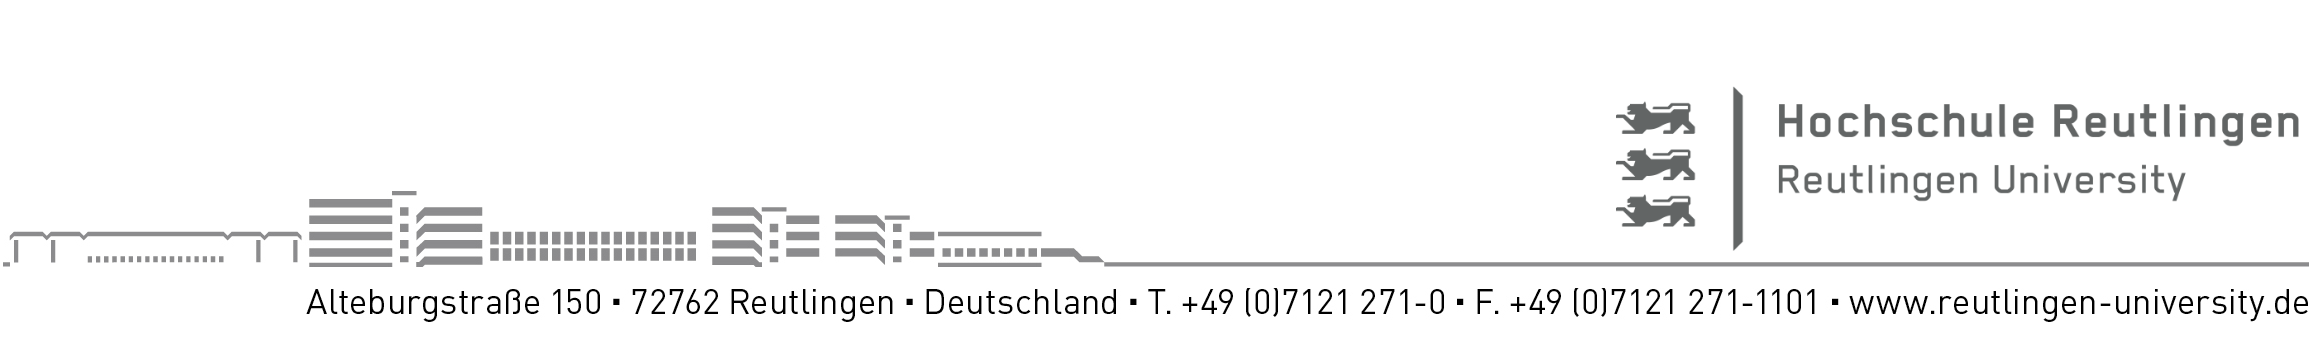
\includegraphics[width=1000pt,height=70pt,keepaspectratio]{images/FHRTFooter.png}
      \end{minipage}%
    }
  }
\end{titlepage}

\newpage
\selectlanguage{german}
\begin{abstract}
  Smart Home sowie Smart Office, die detaillierte Ausprägung des Smart Home, sind Unterrubriken des Internet of Things (IoT). 
  Diese fokussieren die Vernetzung aller Arten von technischen Geräten und die 
  Realisierung verschiedenster Automatisierungsverfahren und Prozessabbildungen. Durch die Vielzahl an Möglichkeiten zur  
  Erfassung von Automationen, Regeln und Geräten kann der Input der Anwender, bzw. Entwickler rasant ansteigen. 
  Es ist dem Anwender meist kaum gestattet mit den vorhandenen Softwarelösungen eine inhaltlich individuelle Anpassung 
  der Regeldefinitionen vorzunehmen. %, wodurch die formalisierten Interaktionen nicht einfach zu handhaben sind. 
  \\
  \linebreak
  Diese Master-Thesis befasst sich mit der Konzeption und prototypischen Umsetzung eines Frameworks einer Steuerzentrale im Rahmen eines 
  intelligenten Büros mit dem Fokus auf eine einfache Handhabung der formalisieren Interaktionen für Softwareentwickler. Das System bietet eine 
  klare Struktur zur Definition von Regeln, sodass individuelle Anwendungsfälle in wenigen Schritten umgesetzt werden können. Die Komplexität dieser ist jedoch 
  abhängig von dem zu realisierenden Prozess und kann durch die formalisierten Interaktionen selbst nicht reduziert werden. 
  \\
  Um die Forschungsfrage im Rahmen dieser Thesis zu beantworten sowie das Ziel dieser Arbeit zu erreichen, werden mehrere Forschungsmethoden 
  angewendet. Es wird ein systematisches Literaturreview durchgeführt, das den aktuellen Stand der Technik in Bezug auf die Forschungsfrage dieser Arbeit eruiert. 
  Anschließend wird eine Zielgruppenanalyse erstellt, sowie Anwendungsfälle entwickelt und Experteninterviews geleitet, wodurch Anforderungen an das System extrahiert und identifiziert werden. 
  Mithilfe der erhobenen Informationen und gewonnenen Ergebnissen wird das Framework konzipiert und prototypisch implementiert. Damit der entstandene Prototyp 
  auf die Usability testbar ist und die Anforderungen als auch die Forschungsfrage evaluiert werden können, werden nach der Implementierung 
  Usability-Tests und abschließende Experteninterviews veranlasst. Diese helfen bei der Evaluation. 
\end{abstract}

\newpage
\selectlanguage{english}
\begin{abstract}
  Smart home and smart office, the detailed form of the smart home, are sub-categories of the Internet of Things (IoT). These focus on the 
  networking of all types of technical devices and the implementation of a wide variety of automation processes and process mapping. 
  Due to the large number of options for recording automations, rules and devices, the input from users and developers can increase 
  rapidly. In most cases, the user is not allowed to adapt the content of the rule definitions individually with the existing software solutions.
  \\
  \linebreak
  This master's thesis deals with the conception and prototypical implementation of a system for a control center within the framework of a 
  intelligent office with the focus on easy handling of formalized interactions for software developers. The system offers a clear structure 
  for defining rules so that individual use cases can be implemented in just a few steps. However, the complexity of these depends on the process 
  to be implemented and cannot be reduced by the formalized interactions themselves.
  \\
  In order to answer the research question in this thesis and to achieve the goal of this work, several research methods are used. A systematic 
  literature review is carried out, which determines the current state of the art in relation to the research question of this work. A target group 
  analysis is created, use cases are developed and expert interviews are conducted, whereby requirements for the system are extracted and 
  identified. With the help of the information collected and the results obtained, the framework is designed and implemented as a prototype. So that 
  the resulting prototype can be tested for usability and the requirements as well as the research question can be evaluated, usability tests and 
  concluding expert interviews are caused after implementation. These help with the evaluation. 
\end{abstract}

\newpage
\selectlanguage{german}
\pagestyle{plain}
\chead{\headmark}
\cfoot{\pagemark}
%\pagestyle{headings}
\pagenumbering{Roman}
\tableofcontents           % Inhaltsverzeichnis hier ausgeben

\newpage
\pagenumbering{arabic}
\chapter{Einleitung}
\label{chap:Einleitung}
    Die folgende Master-Thesis befasst sich mit der Konzepterstellung einer zentralen Steuerzentrale, die 
    dem Entwickler die formalen Interaktionen, weitere Funktionen hinzuzufügen, erleichtern soll. Hierfür werden
    bereits bestehende Plattformen für \acl{SH} analysiert und daraus ein Konzept erstellt, die den Anforderungen 
    entsprechend einen größeren Mehrwert in der Weiterentwicklung der Plattform bietet. Die Umsetzung des ausgearbeiteten 
    Konzeptes wird nur in sehr geringem Maß behandelt.
    \\
    \linebreak
    In diesem Teil der Arbeit wird auf die Motivation des Themas eingegangen. Darüber hinaus 
    werden sowohl die Forschungsfragen als auch die Zielsetzung der Arbeit genauestens dargelegt. Darauf 
    folgend findet eine Übersicht über die Arbeit im Gesamten statt, mit der die Inhalte angerissen werden. 
    Eine nähere Betrachtung des Standes der Technik untermauert die Beweggründe dieser Themenwahl und 
    Ausarbeitung dessen. 

\section{Motivation}
\label{sec:Motivation}
    Jede neu entwickelte Technologie durchlebt im Laufe der Entstehung und Publikation ein enormes Aufsehen. 
    So lange bis diese Technik eine standardisierte Verwendung in der Gesellschaft findet oder sich als 
    unpraktikabel erweist und nicht weiter vorangetrieben oder eingestellt wird. Es wird in der Zeit des 
    Aufkommens und der Forschung viel darüber fantasiert, debattiert und geplant, ohne jedoch die Ausmaße und 
    Resultate der Forschungen und Praktiken abwägen zu können. Durch fehlende Erfahrung und nicht ausgereifte 
    Konzepte werden Höhepunkte und Illusionen erwartet, die zu diesem Zeitpunkt technisch nicht umsetzbar sind. 
    Um solche kühnen Versprechungen und Übertreibungen, sogenannte Hypes, die jede neue technologische Idee 
    mit sich bringt, von dem zu differenzieren was wirtschaftlich umsetzbar ist, werden bestimmte Phasen 
    der Entwicklung durchlaufen. \cite{gartner.2022m}
    \\
    \linebreak
    Die oben erwähnten Phasen der Entwicklung sind in einem sogenannten Hype-Zyklus, engl. Hype-Cycle, dargestellt. 
    Dieser Zyklus ist ein visualisiertes Modell, das die Entwicklung einer neuen Technologie von der Innovation 
    und Entstehung über die Forschung und Umsetzung bis hin zur ausgereiften Marktfähigkeit repräsentiert und so 
    diese Phasen der Entwicklung versinnbildlicht.  
    \\
    Entwickelt wurde der Hype Cycle von der Gartner Inc. Forschungsgruppe. Durch die Mitarbeiterin 
    Jackie Finn wurden die Definitionen der Entwicklungsphasen\footnote{Die Entwicklungsphasen der Gartner Inc. ist unter folgender URL zu finden: "\url{https://www.gartner.com/en/research/methodologies/gartner-hype-cycle}"} 
    geprägt. Diese sind wie folgt in fünf Phasen 
    dargestellt:
    \begin{enumerate}
        \item \textit{Innovationsauslöser, engl. Innovation Trigger}: Ein potentieller technologischer Durchbruch 
        löst die Dinge aus. Frühe Proof-of-Concept (PoC) Ansätze und ein großes Medieninteresse lösen eine 
        erhebliche Publizität aus. Oft gibt es keine brauchbaren Produkte und die Marktreife ist nicht 
        bewiesen. \cite{gartner.2022m}
        \item \textit{Höhepunkt überhöhter Erwartungen, engl. Peak of Inflated Expectations}: Frühe Publizität 
        bringt eine Reihe von Erfolgsgeschichten hervor – oft begleitet von zahlreichen Misserfolgen. 
        Einige Unternehmen ergreifen Maßnahmen; viele nicht. \cite{gartner.2022m}
        \item \textit{Trog der Ernüchterung, engl. Trough of Disillusionment}: Das Interesse schwindet, da 
        Experimente und Implementierungen nicht liefern. Hersteller der Technologie reißen es heraus 
        oder scheitern. Investitionen werden nur fortgesetzt, wenn die überlebenden Anbieter ihre Produkte 
        zur Zufriedenheit der frühzeitigen Anwender verbessern. \cite{gartner.2022m}
        \item \textit{Steigung der Erleuchtung, engl. Slope of Enlightenment}: Mehr Beispiele dafür, wie 
        die Technologie dem Unternehmen zugute kommen kann, beginnen sich zu herauszukristallisieren und 
        werden allgemeiner verstanden. Produkte der zweiten und dritten Generation erscheinen von den 
        Technologieanbietern. Mehr Unternehmen finanzieren Pilotprojekte; Konservative Unternehmen 
        bleiben vorsichtig. \cite{gartner.2022m}
        \item \textit{Plateau der Produktivität, engl. Plateau of Productivity}: Mainstream-Akzeptanz beginnt 
        sich abzuheben. Kriterien zur Bewertung der Lebensfähigkeit des Anbieters sind klarer definiert. 
        Die breite Markteinsetzbarkeit und Relevanz der Technologie zahlen sich eindeutig aus. \cite{gartner.2022m}
    \end{enumerate}
    Nachdem ein innovativer Gedanke den \textit{Höhepunkt überhöhter Erwartungen} passiert hat, z.B. die 
    Revolutionierung der Softwareentwicklung oder Szenarien, wie z.B. die Vollautomatisierung eines Gebäudes 
    oder Service-Roboter die uneingeschränkt interagieren können, die man in der Form nur aus Science-Fiction Filmen kennt, 
    folgt der \textit{Trog der Ernüchterung}. In Folge dessen wird festgestellt, dass die Erwartungen nicht 
    in Gänze übertragbar sind, bzw. nur zu einem geminderten Teil in die Realität umgesetzt werden können 
    und der verfolgte Gedanke an Interesse verliert. Nach erneutem Aufgriff der Technologie findet eine realistischere 
    Beurteilung der Innovation statt, die dazu beiträgt, dass die Technologie wieder an Interesse gewinnt. Die 
    objektive und realitätsnahe Betrachtungsweise formt ein neues und realistisches Bild der Potentiale, als auch 
    der Grenzen. Mit dem neu gewonnenen Maßstab geht die ehemals neue innovative Idee in eine routinierte Technologie über, 
    die an Anerkennung gewinnt und in der breiten Masse akzeptiert wird. Die Technologie erfährt mit steigender 
    Zuwendung eine stetigere Weiterentwicklung, die dann zu einer Community geformt wird. Mit der Erreichung dieses Status 
    befindet sich die Innovation, bezogen auf den Hype Cycle, in der letzten Phase, dem \textit{Plateau der Produktivität}, 
    und bestätigt so die Marktreife. Dieser Zeitpunkt löst die Zukunftsvision auf und es handelt sich um eine am Markt 
    etablierte Technologie.
    \\ 
    \linebreak
    Zum aktuellen Zeitpunkt befindet sich die Technologie rund um Plattformen für intelligente Geräte im privaten als auch im unternehmerischen 
    Bereich, engl. \textit{\ac{SH}} oder \textit{Connected Home}, im Anfangsstadium der letzten Phase, dem sogenannten 
    \textit{Plateau der Produktivität}. Mit zunehmender Akzeptanz werden im Umfeld des Internets der Dinge, engl. 
    \textit{\acl{IoT}}, stetig Szenarien entwickelt, die das Wachstum und die Verwendung von solchen Plattformen vorantreibt. 
    Mit einer immer tiefer gehenden Forschung und Umsetzung von Anwendungsbeispielen werden Bereiche offenbart, die 
    eine solche Plattform im privaten als auch im geschäftlichen Umfeld immer attraktiver gestaltet. Mit steigender  
    Konnektivität und Kompatibilität mehreren Geräten und Gegenständen können Szenarien und Prozessautomatisierungen, wie die 
    Steuerung von Service-Robotern, umgesetzt werden. Der jetzige technologische Fortschritt und die über die Forschungsjahre 
    gesammelten Erfahrungen bringt das Segment der intelligenten Geräte der \acs{IoT} den ursprünglich angedachten 
    Visionen und Ideen näher, sodass ein weiterer Ausbau dieser Technologie und dessen Anwendung stattfindet und sich 
    vollständig in den Markt etabliert. Der finale Schritt der endgültigen Marktreife ist ein faszinierender und wichtiger Grund 
    für meine Motivation, mich dieser Technologie und der dahinterstehenden Theorie zu widmen. Ein weiterer dazu beitragender Aspekt ist 
    die Steuerung und Verknüpfung von Geräten, sowie die Automatisierung von Prozessen innerhalb eines intelligenten Büros, um stetig hinzukommende 
    Anwendungsfälle abdecken und einfach implementieren zu können. Einen Ansatz zu schaffen, der einem Softwareentwickler eine Struktur vorgibt, die 
    in sich jedoch beliebig erweiterbar ist, sodass die Einschränkung von Prozessabbildungen minimiert wird. 
    % !!! Weiterer Grund zur Motivation: Dem Entwickler mehrere Freiheiten bei der Umsetzung von Anwendungsfällen oder Regeln zu 
    % !!! schaffen und die Regeldefinition nicht über ein Zusätzliches Framework abzubilden, sondern eine klar Struktur 
    % !!! vorzugeben, die klar definiert, welche grundlegenden Komponenten zu Erweiterung notwendig sind. Weitere Anpassungen oder 
    % !!! Anwendungsfälle verantwortet der Entwickler selbst. (Einbindung von APIs o.ä.)
    %
    %\\
    %Mit der erzielten Marktreife entstehen Produkte und Lösungen, die bestimme Teile der anfänglichen Idee abdecken. Mit 
    %zunehmender Entwicklung und anfallenden Anforderungen, werden viele Produkte zu groß und haben dadurch die grundlegende 
    %Konzeption und Architektur nicht vorausschauend entwickelt. Daher ist die anfängliche Überlegung und Konzeption essentiell.
    %\\
    %Daher ist ein weiterer Punkt meiner Motivation den Schritt zu gehen, ein Konzept zu entwickeln, dass die Erweiterung eines 
    %solchen Systems basierend auf der Konzeptgrundlage vereinfacht und so die Nutzung für Entwickler zur Weiterentwicklung verbessert.
    %
    % !!! Ein weiterer Punkt meiner Motivation ist die Vereinfachung der Erweiterung einer solchen Zentrale. 
    %Somit soll dem Entwickler bei einer stetigen Erweiterung der Plattform Zeit und Aufwand erleichtert werden. Dadurch können weitere 
    %Anwendungsszenarien und Objekte integriert werden, ohne einen zu großen Entwicklungsaufwand zu erzeugen.   
    \\ 
    \linebreak
    Die Einsatzgebiete von intelligenten Geräten, beziehungsweise die Verwendung von Kompaktlösungen, Plattformen und Steuereinheiten zielen räumlich 
    auf Gebäude, Häuser und Wohnungen ab und bieten viele Verwendungs- und Einsatzmöglichkeiten, die stetig ausgebaut und optimiert werden. 
    Diese sehen wie folgt aus: 
    \begin{itemize}
        \item Komfort
        \item Entertainment
        \item Überwachung und Sicherheit
        \item Steuerung von Prozessen
        \item Management von Automatisierungen (Automationen)
    \end{itemize}    
    Neben der Affinität von \acl{SH} zum \acl{IdD} und der damit einhergehenden Technologie bringt diese Vorteile mit sich, wie z.B. 
    die Modernisierung von Wohn- und Bürogebäuden und die routinierte Ausführung und Abarbeitung von Prozessen, die dem Menschen 
    Aufgaben und Arbeiten abnehmen.
\pagebreak
\section{Forschungsfragen}
\label{sec:forschungsfragen}
    Die in der Arbeit zentral behandelte Forschungsfrage ist wie folgt definiert: 
    \\
    \linebreak
    \textit{F1: Wie kann man die Usability von Prozessautomatisierungen und Regeldefinitionen von SmartHome-Plattformen optimieren, sodass die formalen Interaktionen der Softwareentwickler schneller sind?}
    \\
    \linebreak
    Eine Konkretisierung identifiziert konkret die Herausforderungen existierender Plattformen in Bezug auf die Definition von Regeln und Automatisierungen:
    \\
    \linebreak
    \textit{F1.1: Welche sind die Usability-Herausforderungen existierender Plattformen, bzw. welche Anforderungen würden für eine Optimierung gelten?}
    %-	Wie kann man die Usability von Prozessautomatisierungen und Regeldefinitionen von SmartHome-Plattformen optimieren, so dass die formalen Interaktionen der Softwareentwickler schneller sind?
        %o	Welche sind die Usability-Probleme der existierenden Plattformen? 
        %o	Welche Anforderungen würden für eine Verbesserung einer solchen Plattform gelten?
        % Nicht Bestandteil der eigentlichen Forschungsfrage: 
        % -Reicht eine Kommunikationsschnittstelle als Ausgangspunkt für alle Verbindungen?

    % - Wie kann man die Usability von Smart Home - Plattformen optimieren, sodass die formalen Interaktionen der Softwareentwickler schneller sind? 
    %  - Wie kann ein Framework vorgegeben werden, dass den Entwickler (Anwender) bei der Implementierung von Regeln (und der Erweiterung um 
    %    anwenderbasierte Funktionalitäten) nicht einschränkt?

\section{Zielsetzung der Arbeit}
\label{sec:zielsetzung}
    %TBD Wird zum Schluss geschrieben. 
    %Programmierseitige Möglichkeit um Regeln umzusetzen.
    Das Ziel der Arbeit ist die Erarbeitung eines Konzeptes und die prototypische Implementierung des Frameworks, welches dem Softwareentwickler das 
    Umsetzen von Regeln und zu automatisierende Prozesse im Rahmen der Programmierung erleichtert und in der Ausprägung 
    der Regeln nicht einschränkt. Dabei wird sich an bestehenden Produkten orientiert, die versuchen, diese 
    Automatisierungen für den Nutzer vereinfacht darzustellen. Die aktuellen Praktiken setzen trotz dessen eine starke Lernkurve voraus. 
    %und lässt den Nutzer Regeln und Prozesse nur beschränkt einfach abbilden. 
    Mit dem Framework soll dem Anwender eine Struktur an die Hand gegeben werden, mit der Regeln und Prozesse innerhalb eines 
    smarten Büros einfach abgebildet werden können. Die Abarbeitung von Regeln und Prozessen sollen über das Framework 
    koordiniert werden, sodass der Anwender sich ausschließlich um die Regeldefinition und um die abzubildende Umgebung durch Geräte, Zustände und weitere 
    potentielle Mittel innerhalb eines smarten Büros, kümmern muss. 
    %"Anleitung" dem Entwickler an die Hand zu geben, dass Prozesse schnell umgesetzt werden können und jedoch 
    % keinerlei Einschränkungen hat, da mit Java (Spring Boot) keine Grenzen gesetzt sind und mit dem Framework auch 
    %keine Grenzen gesetzt werden.

    %%%%%%%%%%%%%%%%%%%%%%%%%%%%%%%%%%%%%%%%%%%%%%%%%%%%%%%%%%%%%

    % ZIEL DES KONZEPTES: Ein Framework für Entwickler bereitzustellen, welches die Mächtigkeit für den Entwickler offen lässt, nicht einschränkt 
    % und dennoch Konfiguration und Ausführung umsetzt. Der Entwickler muss lediglich den Zustandsraum, die MQTT-Topics und die Regeln definieren.
    % Der Entwickler bekommt ein Framework in die Hand, welches die Umsetzung von Prozessen in einem smarten Büro ermöglicht. Das Framework kümmert sich um die 
    % Organisation und die Ausführung der Regeln. Die Richtigkeit der Regeln und des Zustandsraumes muss der Entwickler sicherstellen. 
    % Die Kommunikation über MQTT ist nur eine Möglichkeit. Des Setup wird wegabstrahiert 


    %%%%%%%%%%%%%%%%%%%%%%%%%%%%%%%%%%%%%%%%%%%%%%%%%%%%%%%%%%%%%

\section{Forschungsstrategie und Forschungsmethoden}
\label{sec:forschungsstrategie}
    Dieser Abschnitt der Arbeit widmet sich der Forschungsstrategien und der darauf angewendeten Forschungsmethoden. 
    Hierbei werden die Strategien kurz erläutert und die Methoden skizziert. Die Anwendung der Strategien findet zu 
    späterem Zeitpunkt statt. 
    \\
    Diese Arbeit ist in die drei Phasen aufgeteilt, Forschung, Konzeption und Evaluation. Zuerst erfolgt durch ein 
    systematisches Literaturreview eine Analyse des aktuellen Stands der Technik, welche die Forschungsfragen aufgreift und 
    anhand dessen den aktuellen Stand identifiziert. Schwerpunkt dabei liegt auf der einfachen Handhabung der formalisierten 
    Interaktionen eines Softwareentwicklers bei der Weiterentwicklung, bzw. bei der Ergänzung einer bestehenden 
    Softwarelösung, um weitere Anwendungsfälle abzudecken. 
    In der Phase der Anforderungserhebung werden Experteninterviews durchgeführt, mit denen die Anforderungen des Produktes, 
    für welches ein Konzept erstellt wird, identifiziert werden. Ergänzend dazu werden im Rahmen der Arbeit weitere 
    Anforderungen durch das \ac{RE} und der Anwendung des \textit{user-centered design}-Prinzips\footnote{Iterativer Prozess zur Ermittlung von Anforderungen, die nutzerorientiert aufgestellt werden. \url{https://www.interaction-design.org/literature/topics/user-centered-design} Abgerufen am 08.05.2022} 
    sowie des \textit{target group analysis}-Ansatzes (\ref{sec:zielgruppenanalyse}) ermittelt. Dabei wird die 
    Nutzerorientierung auf den Softwareentwickler ausgelegt. 
    Zur anschließenden Evaluation wird ein Usability Test durchgeführt und darauf erneut ein Experten Interview, damit 
    Eindrücke über das Konzept entstehen und die Erfahrungen der Experten während des Usability Tests 
    in die Beantwortung der Forschungsfrage mit einfließen.
    \\
    Die soeben genannten Forschungsmethoden werden im Nachfolgen- den näher erklärt.

    \subsection{Experteninterview}
    \label{subsec:experteninterview}
        Zu Anfang wird bei einem Experten Interview der Hintergrund des Interviews erläutert. Nachdem die interviewende 
        Person den Grund dargelegt hat, stellt ein Forscher einem Experten ausgewählte Interview-Fragen, die für die 
        Forschung relevant sind und dazu beitragen die Forschungsfrage zu beantworten.
        \\
        \linebreak
        Die Interview-Fragen können als offene oder geschlossene Fragen formuliert werden, je nachdem ist eine beliebige Reihe 
        an Antworten möglich oder nur eine begrenzte Anzahl an Antworten \cite{robson2002real}. Der Verlauf des Interviews 
        kann von dem Forscher selbst bestimmt werden. Sind nur bestimmte Antworten gewünscht, so können die Fragen strukturiert und 
        geschlossen formuliert werden. Ebenso gibt es den semi-strukturierten und den unstrukturierten Ansatz, bei dem das Interview 
        offen gestaltet werden kann. Der Semi-Strukturierte Ansatz eignet sich, wenn spezielle Fragen adressiert werden, bzw. eine 
        Reihenfolge festgelegt ist, sodass der Interviewer eine klare Reihenfolge hat. Mit dem unstrukturierten Vorgehen wird 
        ein völlig offenes Interview angestrebt, bei dem der Verlauf abhängig von dem Inhalt der Konversation ist.

    \subsection{Systematisches Literaturreview}
    \label{subsec:systematischesliteraturreview}
        Mit einem systematischen Literaturreview wird zur evidenzbasierten Identifizierung, Bewertung und Interpretation  
        von bestehender Literatur eine wissenschaftliche Methode angewendet, mit der Fragestellungen zu einer bestimmten Thematik 
        herausgearbeitet werden können. Mithilfe diesen Ansatzes soll die Erzielung einer Schlussfolgerung zu einem untersuchten Objekt 
        ermöglicht werden. 
        Die Methodik des systematischen Literaturreviews orientiert sich an den Richtlinen von Kitchenham et al.. Diese ist in drei 
        aufeinander aufbauende Schritte gegliedert. Zu Beginn erfolgt die Planung, anschließend die Durchführung und abschließend die 
        Dokumentation und Offenlegung der Ergebnisse \cite{Kitchenham2007}.

    \subsection{Usability-Test}
    \label{subsec:usabilitytests}
        Ein Usability-Test ist eine Methode zur Testung von Prototypen oder Arbeitsversionen von Computerschnittstellen \cite{LAZAR2017263}. 
        Das Testen der Nutzbarkeit kann durch vorab definierte Aufgaben, die durch Probanden und Benutzer in einer dafür vorgesehenen 
        Umgebung durchgeführt werden, erfolgen. Die Aufgaben können je nach Anwendungsfeld oder -kontext unterschiedlich ausfallen. 
        Ebenso können solche Tests auch dazu beitragen, um physische Interaktionen mit bspw. Geräten zu bewerten. 
        \\
        Alle Ansätze für Usability-Tests haben ein grundlegendes Ziel: Die Qualität einer Schnittstelle zu verbessern und den 
        dafür vorgesehenen Anwendern diese Benutzung so einfach wie möglich zu gestalten \cite{LAZAR2017263}. Während diese Tests optimaler 
        Weise Schnittstellenfehler aufdecken, die den Benutzern Schwierigkeiten bereiten, ist gleichzeitig rauszufinden, welches Schnittstellendesign 
        gut funktioniert, um dieses für Zukünftige Entwicklungen beizubehalten. 
        \\
        \linebreak
        Zur Kategorisierung von durchgeführten Tests, werden Werkzeuge verwendet, die das Verhalten und die Meinungen der Benutzer 
        messbar macht. Eines dieser Werzeuge ist das \textit{System Usability Scale (SUS)}\footnote{System Usability Scale. \url{https://www.usability.gov/how-to-and-tools/methods/system-usability-scale.html} Besucht am 03.07.2022}. 
        Dabei handelt es sich um einen einfachen 
        technologieunabhängigen Fragebogen, anhand dessen die Gebrauchstauglichkeit eines Systems bewertet werden kann. Dieser 
        ist eine Praktik zur quantitativen Analyse der Nutzbarkeit. Der Umfang umfasst zehn Fragen nach der Likert-Skala \cite{likert1932technique}.

\section{Aufbau der Arbeit}
\label{sec:aufbau}
    Die vorliegende Master-Thesis gliedert sich nach den soeben genannten einleitenden Information im Aufbau in insgesamt 
    zehn Kapitel. Das erste Kapitel (\ref{chap:Einleitung}) beschreibt die Motivation (\ref{sec:Motivation}), welche die 
    Intension kundtut, diese Thematik rund um \acs{IoT} und Smart Home zu bearbeiten. Darauf folgend werden die 
    Forschungsfragen (\ref{sec:forschungsfragen}), die im Rahmen der Thesis behandelt werden, erläutert. Nach der 
    Beschreibung der Forschungsfragen wird im anknüpfenden Abschnitt (\ref{sec:zielsetzung}) die Zielsetzung der 
    Arbeit erläutert. Hierbei werden zusätzliche Schwerpunkte und Ziele aufgegriffen. Abschließend wird das Unternehmen, in der 
    die Thesis geschrieben wird, hervorgehoben und deren Absichten in Verbindung mit Innovationen beleuchtet. 
    \\
    \linebreak
    Das Kapitel (\ref{chap:grundlagen}) widmet sich den essentiellen und wichtigen Grundlagen dieser Arbeit. Zu Anfang wird dem 
    Leser der Terminus des \acl{IoT} (\ref{sec:iot}) offenbart, um zum Teil den Kontext im Bezug zu dieser Arbeit zu begreifen, 
    gefolgt von einer Einführung in die Thematik des \acl{SH} (\ref{sec:smartHome}), der Problematik der Begriffsdefinition, der 
    historischen und kontinuierlichen Entwicklung und mit den Zielen, die mit der Verwendung einer Smart Home Lösung bewältigt 
    werden sollen. Mit dem Verständnis der übergeordneten Begriffe, \acs{IoT} und \acl{SH}, werden Technologien 
    (\ref{sec:technologien}) aufgegriffen, die im Rahmen dieser Arbeit erwähnenswert sind und verwendet werden. %Um auf die Vielfältigkeit 
    %von der Umsetzung eines \acl{SH} einzugehen und einen Teilaspekt der Anforderungen Abzudecken, wird ebenso auf Service-Roboter 
    %(\ref{sec:roboter}) eingegangen. 
    Abschließend werden in Kapitel (\ref{chap:grundlagen}) die Softwarelösungen, Home Assistant 
    und openHAB (\ref{sec:homeassistant} \& \ref{sec:openhab}), dargestellt. Diese dienen zur Grundlage für die Evaluation als 
    auch zur Gegenüberstellung der Lösungen in Kapitel (\ref{chap:evaluation}) Diskussion und Evaluation. 
    \\
    \linebreak
    Die theoretischen und methodischen Hintergründe sowie den Stand der Technik wird in Kapitel (\ref{chap:technikStand} )
    angesprochen. Dieser Teil enthält Beschreibungen, Forschungen und aktuelle Erkenntnisse über Technologien, die im Umfeld der 
    Smart Home Anwendungen innerhalb des \acs{IoT} verwendet werden. Zudem werden in Zusammenhang der Erkenntnisse und 
    Möglichkeiten der Technologie die Szenarien dargestellt. 
    \\
    \linebreak
    Kapitel (\ref{chap:anforderungsanalyse}) befasst sich mit den Anforderungen, engl. Requirements, die für die 
    eigentliche Konzeption relevant sind. Innerhalb dieses Kapitels wird anhand von Informationen und den umzusetzenden 
    Szenarien die Anforderungen für die Konzeption erarbeitet. Hierbei werden aus der Praxis bekannte Verfahren verwenden, um 
    die Anforderungen zu definieren. Mittels den zugrundeliegenden Anforderungen wird im nachfolgenden Schritt die eigentliche 
    Konzeption dargelegt.
    \\
    \linebreak 
    Nach Aufbereitung der Anforderungen durch das sogenannte Anforderungsmanagement, engl. \textit{Requirements Engineering},
    wird in Kapitel (\ref{chap:konzept}) das Konzept erarbeitet, welches als Grundlage für die prototypische Implementierung und 
    Umsetzung des Konzepts dient. Das Konzept befasst sich mit den Anforderungen und setzt diese ein, um die Organisation des 
    Systems in Komponenten, deren Beziehungen zueinander und zur Umgebung sowie deren Prinzipien zu definieren. Zum Ende des 
    Konzepts steht eine Architektur, die sich aus den Anforderungen und auch aus den Analysen der eigentlichen Forschungsfrage 
    abzeichnet.
    \\
    \linebreak
    In Kapitel (\ref{chap:umsetzung}) wird die Umsetzung des Konzepts skizziert. Darunter welche Problem während der Implementierung 
    auftraten als auch deren Lösungsfindung. Ebenso wird hier aus praktischer Sicht auf die Architektur geschaut, welche Komponenten,  
    Bibliotheken und zusätzliche Systeme, engl. \textit{Frameworks}, verwendet wurden. Das erzielte Ergebnis und Resultat wird 
    abschließend zusammengefasst und neutral betrachtet.
    %\\ 
    %\linebreak
    %Das Ergebnis wird aus objektiver Sicht in dem darauf folgenden Kapitel (\ref{chap:ergebnis}) erläutert. 
    \\
    \linebreak
    Nach Abschluss der Umsetzung und dessen Ergebnisdokumentation befasst sich das Kapitel (\ref{chap:evaluation}) mit der Diskussion 
    und Evaluation. Hier findet eine Analyse des Konzepts sowie deren Umsetzung und objektive Betrachtung statt. Anschließend werden 
    Vergleiche zwischen der Eigenentwicklung und bereits bestehender Softwarelösungen, die im Grundlagenkapitel aufgefasst werden, 
    aufgestellt und bewertet. %Testdurchführung und anschließende Evaluation (Experten Interview)
    \\
    \linebreak
    Im vorletzten Teil, Kapitel (\ref{chap:fazit}), wird ein Fazit aus den Erkenntnissen und Ergebnissen gezogen. Dieses Schlussresümee 
    führt nochmals die Höhepunkte sowie eine eigene Einschätzung auf. 
    \\
    \linebreak
    Zum Abschluss der Thesis wird in Kapitel (\ref{chap:ausblick}) ein Ausblick gegeben. Dieser gibt Aufschluss darüber, welche 
    Erweiterungsmöglichkeiten es für die in dieser Thesis erfolgten Arbeit gibt und wie innovativ sich dieser Grundbaustein in Zukunft 
    erweisen könnte. 

%\section{CGI}
%\label{sec:cgi}
%\section{Forschungsfragen}
Hallo
%\section{Zielsetzung der Arbeit}
Zielsetzung / Zielerreichung
%\section{Aufbau der Arbeit}
Hallo Test
\chapter{Grundlagen}
\label{chap:grundlagen}
    In diesem Kapitel werden die für diese Thesis relevanten Grundlagen geschaffen, um ein Grundverständnis und 
    fundiertes Wissen über verwendete Technologien zu erlangen und die nachfolgende Recherche, Konzeption und 
    Umsetzung besser verstehen zu können. 

    % Beschreibung
    % Definition
    % Gesamtbild 
    % Historische Entwicklung 

\section{Internet der Dinge}
\label{sec:iot}
    Das \ac{IdD}, im Englischen \ac{IoT}, zählt als eines der Schlagworte in der \ac{IT}. In der Domäne des \acs{IoT} bekommen 
    Gegenstände und Objekte eine eindeutige Identität, die eine Kommunikation miteinander als auch das Entgegennehmen von 
    Befehlen erlaubt. Mit dem \acl{IdD} lassen sich Anwendungen sowie Prozesse automatisieren und Aufgaben erledigen ohne das 
    von außen Eingegriffen werden muss \cite{bigdatainsider2016}. Die Prozessautomatisierung findet sich auch im Kontext des 
    \acl{SH} wieder, welches in nachfolgendem Kapitel genauer aufgegriffen wird. 
    \\
    \linebreak
    In der einschlägigen Literatur gibt es für das \acl{IoT} keine allgemeingültige Definition die alle Anwendungsbereiche abdeckt. 
    Die Definitionen und Auslegungen der Interpretation unterscheiden sich je nach Anwendungsgebiet. Demnach gibt es viele verschiedene 
    Forschungsgruppen, darunter Forscher, Akademiker, Innovatoren, Entwickler und Geschäftsleute, die den Begriff oder die zugrundeliegende 
    Problemstellung definiert haben. Die Ursprünge jedoch sind dem Experten für digitale Innovationen, Kevin Ashton\footnote{Britischer Technologie-Pionier, Mitgründer des Auto-ID Centers am Massachusetts Institute of Technology (MIT). \url{https://de.wikipedia.org/wiki/Kevin_Ashton} (Abgerufen am 22.03.2022)}, 
    zuzuschreiben. 
    \\ 
    Die in der Literatur auffindbaren Definitionen verfolgen zwei Sichtweisen, zum Einen aus Sicht des aktiven, dass die Daten von 
    Menschen erstellt wurde, zum Andere, aus Sicht des passiven, dass die Daten von Dingen, darunter die Sensoren und Aktoren, 
    erstellt wurde. \cite{Madakam2015} Eine aus dem Zusammenschluss hervorgehende Definition ist, dem wissenschaftlichen Artikel zufolge, folgende:
    % „Ein offenes und umfassendes Netzwerk intelligenter Objekte, die in der Lage sind, sich automatisch zu organisieren, 
    % Informationen, Daten und Ressourcen auszutauschen und auf Situationen und Veränderungen in der Umgebung zu reagieren 
    % und zu handeln.“
    \pagebreak
    \begin{quote}
        “An open and comprehensive network of intelligent objects that have the capacity to auto-organize, share information, data 
        and resources, reacting and acting in face of situations and changes in the environment” \cite{Madakam2015}
    \end{quote}
    Daraus kann abgeleitet werden, dass der Begriff des \acl{IdD} für die Vernetzung von Gegenständen im privaten Gebrauch oder 
    von Geräten und Maschinen im industriellen Umfeld über das Internet steht. Damit Geräte individuell angesprochen werden können, werden diese 
    mit einer eindeutigen Identität, genauer einer \ac{IP}-Adresse, im Netzwerk belegt und mit elektronischer Intelligenz ausgestattet \cite{bigdatainsider2016}.
    Darüber sind die Netzwerkteilnehmer im Stande, über das Internet zu kommunizieren Prozesse automatisiert zu erledigen. Die sogenannten 
    \textit{intelligenten Geräte} werden auch oft mit dem englischen Begriff, \textit{Smart Devices}, betitelt. 
    \\
    \linebreak
    Neben der Kommunikation der Geräte über das Netzwerk untereinander kann ebenso entweder durch das Gerät selbst oder eine zentrale 
    Schnittstelle über das Internet interagiert werden. Dadurch sind Objekte und Gegenstände durch einen Benutzer von beliebigen Orten 
    auch außerhalb des Netzwerks erreichbar und können so bedient werden. Diese Art und Weise wird auch in dem zentralen Thema des 
    \acl{SH} verwendet. Die Funktion als auch die Umsetzung wird im Kapitel (\ref{sec:smartHome}) näher beleuchtet.
    \\
    \linebreak
    Das \acl{IdD} ist ein nahezu existenzielles Konzept der \acs{IT}-Welt. Mit dem \acs{IoT} wird die Vision verfolgt eine globale 
    Infrastruktur zu erstellen, mit dem physische Objekte miteinander vernetzt werden und jeder Zeit zur Verfügung stehen. Das \acl{IoT} 
    kann auch als globales Netzwerk angesehen werden, indem die Kommunikation zwischen Mensch zu Mensch, Gerät zu Mensch und Gerät zu 
    Gerät ermöglicht. In vielen Artikeln wird auch davon gesprochen, dass mit der Technologie die Verschmelzung der digitalen und 
    der physischen Welt vorangetrieben wird.\footnote{Das Internet der Dinge – der digitale Zwilling der Welt. Kompetenzzentrum Öffentliche IT in Kooperation mit dem Fraunhofer Institut. \url{https://www.oeffentliche-it.de/trendsonar-iot} Abgerufen am 23.03.2022.} 
    Die Vereinigung beider Welten ist die Verknüpfung physischer Objekte, die eindeutig identifizierbar sind, mit einer virtuellen 
    Repräsentation in einer vergleichbaren Internet-Struktur. 

    \subsection*{Gesamtbild des \acl{IoT}}
        Der folgenden Abbildung (\ref{pic:mindmap_IoT}) ist zu entnehmen, welche Technologien rund um das \acl{IdD} liegen und in Verbindung damit stehen. 
        \begin{figure}[hbt!]
            \centering
            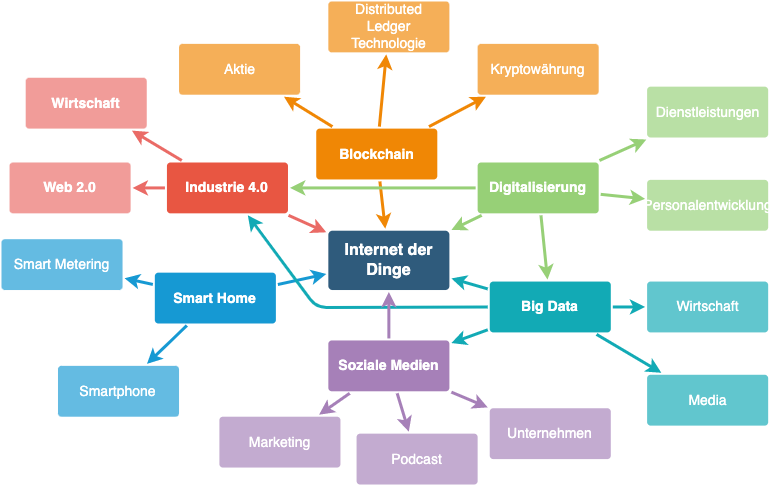
\includegraphics[width=13cm,height=13cm,keepaspectratio]{images/IoT-Mind_Map.png}
            \caption{Technologische Einordnung von IoT \cite{iotmindmap2018}}
            \label{pic:mindmap_IoT}
        \end{figure}
        \\
        \pagebreak
        Beispielsweise ist das \acs{IoT} eine wesentliche Grundlage für das Themengebiet \textit{Big Data}. Die durch Sensoren und Aktoren erzeugten Daten 
        können Grundlage für die Verwendung im Bereich \textit{Big Data} sein. Dabei werden die Datenmengen gespeichert und mithilfe von Mustern 
        und Herangehensweisen des Big Data analysiert. 

    \subsubsection*{Anwendungsbereiche des \acs{IoT}}
        Grundlegend können im Bereich des \acl{IoT} zwischen zwei Anwendungsbereichen unterschieden werden, zum Einen im privaten Bereich und zum 
        Anderen im industriellen Bereich. %Einsteuerung von IIoT% 

        %Grundsätzlich kann beim Internet der Dinge zwischen privaten und industriellen Anwendungen unterschieden werden. Im privaten Umfeld sind 
        %hauptsächlich Gegenstände des alltäglichen Gebrauchs für eine komfortablere und intelligentere Nutzung untereinander vernetzt. Es lassen 
        %sich beispielsweise intelligente Gebäudeautomatisierungen installieren oder Geräte realisieren, die bei bestimmten Ereignissen per Internet 
        %mit dem Anwender in Kontakt treten.
    
        %Im industriellen Bereich geht es hauptsächlich darum, Maschinen und Anlagen so miteinander zu verbinden, dass sich ganze Industrieprozesse 
        %automatisieren lassen. Produktionsabläufe werden dadurch effizienter und günstiger. Das Internet der Dinge ist eine elementare Komponente 
        %der so genannten Industrie 4.0. Mit dem IoT und Industrie 4.0 wird die Selbstorganisation von industriellen Prozessen durch die direkte 
        %Kommunikation von Maschinen, Anlagen, Waren und Menschen möglich. Es lassen sich nicht mehr nur einzelne Produktionsschritte, sondern 
        %ganze Wertschöpfungsketten automatisieren und wesentlich effizienter gestalten.




    %\subsection{IIoT}

\subsection{Edge und Cloud Computing}
    %Definition Edge Computing
    %Definition Cloud Computing
    % Unterschiede der beiden Ansätze und in Zusammenhang mit IoT (kurz)

\subsection{Ziele von \acs{IoT}}
%\section{Smart Home}
\label{sec:smartHome}
    \acl{SH}, übersetzt in Deutsch \textit{“intelligentes Zuhause“}, ist einer von mehreren bekannten Zweigen des \acs{IoT}s. 
    Speziell diese Rubrik widmet sich explizit 
    sämtlichen Haushaltsgeräten und -einrichtungen. Aus diesem Grund können viele Geräte ebenso intelligente Gegenstände 
    der Rubrik \acl{SH} sein. Ein kleiner Ausschnitt solcher Nutzgegenstände sind unter anderem Lampe, Kontaktsensoren, 
    Thermostate, Service-Roboter, Staubsauger-Roboter, Kühlschränke Geräte rundum die Haussicherheit. 
    \\ 
    Unter dem Oberbegriff \acl{SH} ist auch eine Weise zu verstehen, mit der die Erhöhung der Wohn- und Lebensqualität, 
    effizienteren Energienutzung unter Verwendung vernetzter und fernsteuerbarer Geräten, Sicherheit sowie automatisierbaren 
    Abläufe gesteigert werden kann. 
    \\ 
    Der Begriff intelligenten Zuhause wird auch schon verwendet, wenn die Haustechnik und Haushaltsgeräte unter einander  
    vernetzt sind. Die Definition im Deutschen Gebrauch, welche nach (Strese et al. 2010) in der Untersuchung im Rahmen 
    der wissenschaftlichen Begleitung zum Programm Next Generation Media (NGM) des Bundesministeriums für Wirtschaft und 
    Technologie aufgegriffen wird, lautet wie folgt: 
    \begin{quote}
        „Das Smart Home ist ein privat genutztes Heim (z.B. Eigenheim, Mietwohnung), in dem die zahlreichen Geräte der 
        Hausautomation (wie Heizung, Beleuchtung, Belüftung), Haushaltstechnik (wie z.B. Kühlschrank, Waschmaschine), 
        Konsumelektronik und Kommunikationseinrichtungen zu intelligenten Gegenständen werden, die sich an den 
        Bedürfnissen der Bewohner orientieren. Durch Vernetzung dieser Gegenstände untereinander können neue 
        Assistenzfunktionen und Dienste zum Nutzen des Bewohners bereitgestellt werden und einen Mehrwert 
        generieren, der über den einzelnen Nutzen der im Haus vorhandenen Anwendungen hinausgeht.“ \cite{strese.2010m}
    \end{quote}
    Eine vergleichbare Definition wurde zu späterem Zeitpunkt durch eine Literaturrecherche publiziert. Diese beschreibt 
    die zugrundeliegende Thematik weniger aus Anwendersicht sonder widmet sich vielmehr dem System und der Konnektivität. 
    \begin{quote}
        „A smart home is a place with heterogeneous systems to many
        front devices with the support of embedded information and
        communication architectures[...]“ \cite{Balakrishnan2018}
    \end{quote}
    Den beiden Definitionen ist zu entnehmen, dass die Kernaussage eine ähnliche ist, es jedoch in Büchern, Fachartikeln, 
    Publikationen an Universitäten und in den verbreiteten Medien bis heute keine durchgängige Definition gibt. Aus der 
    empirischen Literatur wird ersichtlich, dass viele Synonyme für die Benennung der Thematik verwendet werden, darunter 
    beispielsweise: \cite{strese.2010m}
    \begin{itemize}
        \item Connected Home
        \item Elektronisches Haus
        \item Intelligentes Haus (engl. Smart House)
        \item Smart Living
        \item Home of the Future 
    \end{itemize}
    
\section{Technologien}
\label{sec:technologien}
    Die bereits angesprochene Kommunikation und Vernetzung zwischen Geräten basiert im Allgemeinen auf 
    diversen Protokollen. Um diese Datenbewegung und Kommunikation besser verstehen zu können, werden im 
    Folgenden bekannte Protokolle erwähnt und aufgeführt und eines der meist verwendeten näher betrachtet. 
    Um einen Vergleich herzustellen, wird ein vergleichbares Protokoll betrachtet. Diese werden dann zum 
    Abschluss gegenübergestellt. 

    \subsection{Übertragungsmethoden}
    \label{subsec:netzwerkprotokolle}
    Allgemein gibt es im Bereich des \acl{SH} mehrere Methoden und Möglichkeiten, die Objekte miteinander zu vernetzen. 
    Unter dessen gehören Protokolle über Bluetooth, Ethernet, WLAN, Bussysteme, Funk und Stromleitung. 
    Diese werden Abhängig von den Herstellern eingesetzt. Proprietäre Systeme funktionieren nur über eine 
    Übertragungsmethode. So erzwingen die Hersteller die Nutzung einer Produktlinie, bzw. den Kauf einer 
    einheitlichen Lösung. Geräte die die Möglichkeiten besitzen über mehrere Protokolle 
    zu kommunizieren sind flexibler einsetzbar und mit mehreren Plattformen und Geräten kompatibel.
    Grundlegend werden mit diesen Übertragungsmethoden Netzwerke erstellt, über das die Geräte in einem \acl{SH} kommunizieren können.
    Die populärsten werden in folgender Tabelle aufgelistet: 
    \begin{table}[hbt!]
        \begin{center}
            \begin{tabular}{| p{3.25cm} | p{3.25cm} | p{3.25cm} | p{3.25cm} |}
                \hline
                    \textbf{Technologie} & \textbf{Übertragung} & \textbf{Frequenzbereich (Funk)} & \textbf{Proprietär} \\
                \hline
                    ZigBee & Funk & 2,4 GHz, 868 MHz & Nein \\ 
                \hline
                    Z-Wave & Funk & 868 MHz & Nein \\ 
                \hline
                    HomeMatic & Funk / Datenleitung & 868,3 MHz & Ja \\
                \hline
                    KNX & Funk / Strom- und Datenleitung & 868 MHz / - & Nein / Ja (Datenleitung als Gesamtsystem) \\
                \hline
                    Wi-Fi / WLAN & Funk & 2,4 - 5 GHz & Nein \\
                \hline 
                    Bluetooth & Funk & 2,4 GHz & Nein \\
                \hline
                    io-homecontrol & Funk & 868-870 MHz & Ja \\
                \hline
            \end{tabular}
        \end{center}
        \caption{Übertragungsmethoden des Smart Home}
        \label{tab:protocolsSH}
    \end{table}
    \\
    Die Auflistung der zum aktuellen Zeitpunkt am meist verwendeten Übertragungsmethoden dient 
    lediglich als Einblick, damit eine große Gesamtübersicht der Technologien und der Thematik \acl{SH} entsteht. 
    Demnach wird im Rahmen dieser Arbeit das Thema oberflächlich erläutert und nicht ausführlich vertieft.
    %ZigBee? Erläuterung etwas detaillierter?

    % https://www.bigdata-insider.de/so-laeuft-der-datenaustausch-zwischen-edge-und-cloud-a-1097887/ 

    \subsection{MQTT}
    \label{subsec:mqtt}
        Das \ac{MQTT}-Protokoll ist eines der ältesten offenen Netzwerk- und Nachrichtenprotokolle der 
        \ac{MtoM}-Kommunikation. 
        Dies wurde 1999 von IBM Mitarbeiter Andy Stanford-Clark\footnote{Informationen zu Herrn Stanford-Clark \url{https://stanford-clark.com} Abgerufen am 12.04.2022} 
        und von Cirrus Link Solutions Mitarbeiter Arlen Nipper\footnote{Informationen zu Herrn Nipper \url{https://www.inductiveautomation.com/resources/podcast/the-coinventor-of-mqtt-arlen-nipper-from-cirrus-link-solutions} Abgerufen am 12.04.2022} 
        entwickelt. Die Technologie ermöglicht die Übertragung von Messdaten, sogenannten Telemetriedaten, in Form von 
        Nachrichten zwischen Maschinen und Geräten. Die erzeugten Messdaten durch beispielsweise Sensoren und Aktoren 
        können durch ihre minimale Größe und die kompakte Form des Protokolls in einem kleinen Datenpaket auch bei 
        hoher Verzögerung oder bei beschränktem Netzwerk übertragen werden \cite{Naik2017}. \acs{MQTT} ist ein 
        klassisches Client-Sever-Protokoll, welches nach dem \textit{Publish/Subscribe} Kommunikationsmodell 
        entwickelt wurde. Ein \acs{MQTT}-Client veröffentlicht Nachrichten an einen \acs{MQTT}-Server, den sogenannten 
        \acs{MQTT}-Broker. Diese können von anderen Clients abonniert oder auf dem Broker für zukünftige Abonnements 
        aufbewahrt werden. Jede erzeugte Nachricht wird an eine Adresse veröffentlicht, die als Thema, im Englischen \textit{Topic}, 
        bezeichnet wird \cite{Naik2017}. \acs{MQTT}-Clients können mehrere Topics abonnieren und erhalten jede Nachricht, die an das 
        jeweilig abonnierte Topic gesendet wird. 
        \\
        Die Leichtgewichtigkeit des Protokolls ermöglicht es, die Nachrichten bei eingeschränkter Netzwerkverfügbarkeit zu 
        übermitteln. Ausschlaggebend dafür ist das binär-basierte Protokoll, welches normalerweise einen festen Header von 
        zwei Bytes mit kleinen Nachrichtennutzlasten von maximal bis zu einer Grüße von 256 MB \cite{Naik2017} enthält. Grundlegend 
        ist \acs{MQTT} auf der Basis des Transportprotokoll \ac{TCP} aufgebaut und nutzt zur Verstärkung der Sicherheit die 
        \ac{TLS}/\ac{SSL}-Verschlüsselung. Dadurch sind Client und Broker mit ihrer Kommunikation verbindungsorientiert.  
        Die Anwendung von \acs{MQTT} im Bereich des \acl{SH} zeichnet sich durch die Möglichkeit aus, große Netzwerke mit 
        vielen kleineren Geräten, die von einem Backend-Server, bzw. dem Backend-System überwacht und gesteuert werden müssen, zu 
        betreiben. Dennoch ist es nicht für Mulitcast-Daten oder Übertragungen von Gerät zu Gerät ausgelegt. Die Nutzbarkeit 
        von \acs{MQTT} ist aufgrund der wenigen Steueroptionen und der Einfachheit des Messaging-Protokolls sehr simplen und 
        leichtgewichtig \cite{Naik2017}. 
        \\
        \linebreak
        Ein interessanter Aspekt des \acs{MQTT}-Brokers ist, dass er die gesamte Datenlage seiner Kommunikationspartner aufbewahrt und 
        so die Option bietet, zusätzlich als Zustand-Datenbank betrieben werden kann. Dadurch können weniger leistungsfähige Geräte 
        mit einem \acs{MQTT}-Broker verbunden werden, bei denen die Geräte Befehle und Daten entgegennehmen können, zugleich aber ein 
        komplexeres Lagebild auf dem Broker entsteht. So können Daten an einen leistungsfähigeren Kommunikationspartner 
        weitergeleitet und dort ausgewertet werden.\footnote{\url{https://mqtt.org} Abgerufen am 13.04.2022}
        \\
        Mit diesem Aspekt können durch das \acl{MQTT} Protokoll Automatisierungslösungen geschaffen werden und findet dadurch im 
        Segment \acs{IoT} und \acl{SH} einfache Verwendung und dementsprechend eine große und schnelle Verbreitung. 
        \\
        \linebreak
        Zusammengefasst ist der \acs{MQTT}-Broker die Kommunikationsschnittstelle der \acl{SH}-Geräte und der \acl{SH}-Plattform. 
        Alle Kommunikationspartner können so Informationen (Nachrichten / Messages) auf bestimmte Topics (Endpunkten) senden und 
        diese abonnieren (publish / subscribe). 

        \subsubsection*{Publish/Subscribe Kommunikationmodell}
        \label{subsubsec:pubsub}
            Das Prinzip des Publish/Subscribe Kommunikationsmodells besteht darin, dass Komponenten, die daran 
            interessiert sind, bestimmte Informationen zu konsumieren, ihr Interesse anmelden \cite{Hunkeler2008}. Dieser Vorgang wird als 
            Abonnement (subscription) bezeichnet. Geräte, die an dem Vorgang oder an bestimmten Informationen interessiert sind, 
            werden als Abonnenten (subscriber) definiert. Im Gegenzug können Geräte und Komponenten bestimmte Informationen produzieren und 
            diese veröffentlichen (publish) und an bestimmte Abonnenten weitergeben. Diese Vermittlung der Informationen zwischen 
            Herausgeber (publisher) und Abonnent (subscriber) erfolgt über den Markler (broker), dieser koordiniert sämtlichen Abonnements. 
            Alle Abonnent müssen sich explicit bei dem Broker anmelden, um die Informationen zu erhalten \cite{Hunkeler2008}. 
            \begin{figure}[hbt!]
                \centering
                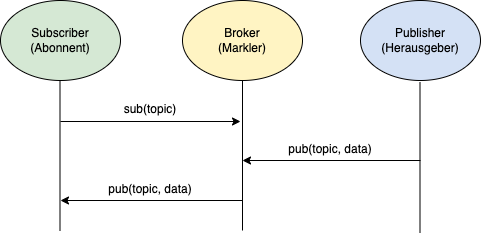
\includegraphics[width=12cm,height=12cm,keepaspectratio]{images/sub-model.drawio.png}
                \caption{Themenbasiertes Pub/Sub Kommunikationsmodell \cite{Hunkeler2008}}
                \label{pic:pub-sub-model}
            \end{figure}
            \\
            Dieses Prinzip ist ein essentieller Bestandteil des \acs{MQTT}-Protokolls. Im Folgenden wird ein Beispiel aufgezeigt, welches 
            die Kommunikation über das Publish/Subscribe Modell darstellt.
            
            \subsubsection*{Beispiel}
            \label{subsubsec:pubsub-example}
            IST NOCH AUSZUARBEITEN. BEISPIELBESCHREIBUNG FOLGT!!!! 
            %TBD 
            \begin{lstlisting}[language=Java, frame=lines, xleftmargin=\parindent, style=algoBericht, label={code:entity}, captionpos=b, caption={Test test}]
                subscribe -topic: test/test/
            \end{lstlisting}
            % Erläutern des Beispiels anhand des publishen und subscriben eines topics in bezug auf das checkin mit der authentifizierung und dem 
            % Command an Temi, welcher dann die Begrüßung und das Checkin durchführt. 


    \subsection{AMQP}
    \label{subsec:amqp}
        Das \ac{AMQP}-Protokoll ist ebenso ein leichtgewichtiges \acs{MtoM}-Protokoll, welches im Jahre 2003 von John O\'Hara JPMorgan Chase 
        in London, Großbritannien, entwickelt wurde \cite{Naik2017}. Der Fokus diesen Protokolls liegt auf der Unternehmens-Messaging Ebene 
        und legt hohen Wert auf die Zuverlässigkeit, Sicherheit, Bereitstellung und Interoperabilität der Kommunikation. \acs{AMQP} 
        unterstützt neben der Publish/Subscribe- auch die Request/Response Architektur. Es bietet eine breite Palette von 
        Funktionen im Zusammenhang mit Messaging, wie z. B. zuverlässiges Queuing, themenbasiertes Publish-and-Subscribe-Messaging, 
        flexibles Routing und Transaktionen \cite{Naik2017}. Das Kommunikationsmodell nach dem \acs{AMQP} Standard erfordert, dass der 
        Herausgeber (publisher) oder der Empfänger (subscriber) einen \textit{Austausch (exchange)} mit einem bestimmten Namen generiert 
        und diesen dann sendet \cite{Naik2017}. Die beiden Komponenten, Empfänger und Herausgeber, nutzen den Namen des Austausch, um eine 
        Verbindung aufzubauen. Der Empfänger erstellt darauf eine Warteschlange (queue) und hängt diese an den Austausch an. Nachrichten, die 
        über diese Verbindung ausgetauscht werden, müssen über einen gesonderten Prozess (binding) mit der Warteschlange abgeglichen werden 
        \cite{Naik2017}.
        \\ 
        Das binäre Protokoll \acs{AMQP} erfordert einen Header von acht Byte mit Nachrichtennutzlasten, die die Größe der Nachricht ist abhängig 
        von dem Broker, bzw. dem Server. Die Verbindungsorientierte Kommunikation von \acs{AMQP} basiert auf dem Standard-Transportprotokoll 
        \acs{TCP} und zur Sicherheit auf dem \acs{TLS}/\acs{SSL}-Protokoll. Ein Kernmerkmal des \acs{AMQP} Kommunikationsmodells ist die 
        Zuverlässigkeit \cite{Naik2017}. 
        \\
        \linebreak
        Neben den beiden aufgeführten Kommunikationsmodellen gibt es noch weitere, darunter das klassische \ac{HTTP} und das \ac{COAP}, die 
        allerdings nicht weiter ausgeführt werden. Der Fokus in dieser Arbeit liegt auf dem \acs{MQTT}-Protokoll. 
        
        %Vergleich in den Anhang packen??
        %\subsubsection*{Vergleich von MQTT und AMQP}
        %\label{subsubsec:mqtt-vs-amqp}
        %\begin{table}[hbt!]
        %    \begin{center}
        %        \begin{tabular}{| p{3.25cm} | p{6cm} | p{6cm} | }
        %            \hline
        %                \textbf{Kriterium} & \textbf{MQTT} & \textbf{AMWP}\\
        %            \hline
        %                Jahr & 1999 & 2003 \\ 
        %            \hline
        %                Architektur & Client/Broker, & Client/Broker Client/Server \\ 
        %            \hline
        %                Abstraktion & Publish/Subscribe & Publish/Subscribe Request/response \\ 
        %            \hline
        %                Header Größe & 2 Byte,  & 8 Byte \\ 
        %            \hline
        %                Nachrichtengröße & max. 265 MB & Abhängig von Broker/Server \\ 
        %            \hline 
        %                Semantik / Methoden & Connect, Disconnect, Publish, Subscribne, Unsubscribe, Close & Consume, Deliver, Publish, Get, Select, Ack, Delete, Nack, Recover, Reject, Open, Close \\
        %            \hline
        %                Zwischenspeicher (Cache) und Proxy & Teilweise & Ja \\
        %            \hline
        %                Standards & OASIS, Eclipse Foundation  & OASIS, ISO/IEC \\ 
        %            \hline
        %                Transport-Protokoll & TCP, & TCP, SCTP \\
        %            \hline
        %                Sicherheit & TLS/SSL & TLS/SSL \\ 
        %            \hline
        %                Standard-Port & 1883/8883 (TLS/SSL) & 5671 (TLS/SSL), 5672 \\
        %            \hline
        %                Format & binär  & Binär \\ 
        %            \hline
        %                Lizenzmodell & Open Source & Open Source \\
        %            \hline
        %                Support & IBM, Facebook, Eurotech, Cisco, Red Hat Amazon (AWS) etc. & Microsoft, JP Morgan, Bank of America, Barclays, Goldman Sachs Credit Suisse \\ 
        %            \hline
        %        \end{tabular}
        %    \end{center}
        %    \caption{Vergleich von MQTT und AMQP \cite{Naik2017}}
        %    \label{tab:mqtt-vs-amqp}
        %\end{table}
        
        
        %Dadurch wird die Konfiguration und Einsetzbarkeit der Technologie komplexer im Gegenzug zu MQTT


        % Vergleich zu MQTT

    
    % Überlegen, bzw. abwarten, ob das benötigt wird.... 
    %\subsection{Raspberry Pi}
    %\label{subsec:raspberrypi} 

%\section{Roboter}
\subsection{Serviceroboter}
\subsection{Temi - Roboter}
\section{Home Assistant}
\label{sec:homeassistant}
    Eines der populärsten \acl{SH} Plattformen ist das sogenannte Home Assistant System. Die Open-Source-Software ist ein zentrales 
    Steuerungssystem von Heimautomationen und der Verwaltung von intelligenten Geräten mit dem Fokus der lokalen Steuerung und gesicherter 
    Privatsphäre. Der Zugriff kann über die Smartphone-App, jeweils verfügbar für iOS und Android, oder auch über die webbasierte 
    Benutzeroberfläche (Web-App) erfolgen. In dem lokalen System können auch Geräte die Steuerung per Sprachbefehlen ermöglichen. Kompatible 
    Plattformen sind unter anderem Google Assistant, Amazon Alexa und Apple HomeKit. Dies sind weitaus nur eine Selektion von bekannten 
    Herstellern. Home Assistant bietet eine weitaus vielfältigere Verknüpfung von Geräten, Services und Plattformen. Die zentrale Steuerung 
    unterstützt durch modulare Integrationskomponenten die einzelnen Geräte, Anwendungen und Services. Für die drahtlose Kommunikation 
    werden native Integrationskomponenten verwendet, darunter Bluetooth, ZigBee und Z-Wave. Diese werden verwendet, um lokale \ac{PAN} mit 
    Geräten mit geringem Stromverbrauch aufzubauen. Die Steuerung kann auch mit Proprietären Ökosystemen stattfinden, sofern diese eine offene 
    \acs{API} oder Anbindungen über \acs{MQTT} anbieten.\footnote{Grundlegende Ableitung der Definition von Home Assistant siehe \url{https://en.wikipedia.org/wiki/Home_Assistant} Abgerufen am 16.04.2022}
    \\
    Die Platform ist in Python geschrieben und wird aktiv instand gehalten und durch eine große Community unterstützt. Die Software ist allgemein unter 
    der Apache 2.0, veröffentlicht. Der folgende Abschnitt befasst sich in Kürze mit der Historie des Systems. 
    
    \subsection*{Historie}
    \label{sec:historyHOAS}
        Anfang des vierten Quartals im Jahr 2013 startete das Python-Projekt von Paulus Schoutsen und im November 2013 erstmals auf GitHub 
        veröffentlicht.\footnote{Anfänge von Home Assistant. \url{https://www.linux.com/topic/embedded-iot/home-assistant-python-approach-home-automation/} Abgerufen am 18.04.2022}
        \\
        \linebreak
        Vier Jahre nach den ersten Entwicklungen der \acl{SH} Plattform wurde im Juli 2017 ein verwaltetes Betriebssystem mit dem Namen 
        \textit{Hass.io} entwickelt.\footnote{Verkündungen von Home Assistant. \url{https://www.home-assistant.io/blog/categories/announcements/} Abgerufen am 18.04.2022} 
        Dadurch gelang der Durchbruch der vereinfachten Verwendung von der Home Assistant Plattform auf kleineren Computern, sogenannten 
        Einplatinencomputern, wie beispielsweise einem der Raspberry Pi Serie. In Zusammenhang mit dem Betriebssystem kam ein 
        \textit{Supervisor}-Verwaltungssystem hinzu, das den Benutzern die Verwaltung, Sicherung und Aktualisierung der lokalen Installation 
        ermöglicht. Ein weiteres Feature des Supervisors ist die Möglichkeit der Plattform über Add Ons weitere Funktionalitäten zu Verfügung zu 
        stellen.\footnote{Einstieg in das Hass.io Betriebssystem. \url{https://www.home-assistant.io/blog/2017/07/25/introducing-hassio/} Abgerufen am 18.04.2022}
        \\
        \linebreak
        Die Software wird stetig weiterentwickelt und verbessert. Mittlerweile gehört sie zu den am meist genutzten Open-Source-Plattformen 
        im Bereich \acl{SH}.

\subsection{Konzept und Architektur}
\label{sec:conceptArchitectureHAOS}
    Home Assistant bietet eine Plattform für die zentrale Haussteuerung und die damit einhergehende Steuerung von Heimautomationen. Die 
    Software ist nicht nur eine einfache Steuerungs- und Konfigurations-Software, sondern ein eingebettetes Betriebssystem, das 
    verbraucher- und nutzerorientiert das Verwenden und Konfigurieren von Haussteuerungen erleichtert. \footnote{Konzept und Architektur von Home Assistant. \url{https://developers.home-assistant.io/docs/architecture_index} Abgerufen am 19.04.2022}
    \\
    \linebreak
    Damit der offene Ansatz von Home Assistant Anbietern gegenüber nicht eingeschränkt ist, bietet die Software Möglichkeiten, um viele 
    Geräte zu vereinheitlichen. Somit begegnet Home Assistant der Heterogenität des offenen Marktes, in sofern, dass diese Geräte auf  
    gemeinsame Konzepte gebracht werden. Diese sind in vier Konzepte\footnote{Erläuterung der Konzepte von Home Assistant. \url{https://apiumhub.com/tech-blog-barcelona/domotics-with-home-assistant-concepts/} Abgerufen am 21.04.2022} 
    aufgeteilt, mit der die Vereinheitlichung vorangetrieben werden kann: 
    \begin{itemize}
        \item Integration (Integration): Integrationen repräsentieren die Geräte und Dienste innerhalb der Home Assistant Anwendung. 
              Ebenso können mittels den Integrationen auch Daten von Datenpunkten abgerufen werden.
        \item Gerät (Device): Nach der Konfiguration der Integration werden die Geräte in Home Assistant angelegt. 
              Diese werden dann als erkannte Geräte der Integration dargestellt, z.B. als Temperatur-, Licht- oder Feuchtigkeitssensor.
        \item Entität (Entity): Die Datenpunkte sind die Geräte, die sogenannten Entitäten, die durch die Integrationen standardisiert werden. 
              Dies sin Objekte, die Funktionalitäten oder Daten des Geräts darstellen, z.B. die Temperatur, Helligkeit oder die Feuchtigkeit.
        \item Automatisierung (Automation): Automatisierungen sind Prozesse, die bei einem bestimmten ausgelösten Event ausgeführt werden 
              sollen. Dieses Auslöser (trigger) können Zeitpunkte, Ereignisse oder manuell gesteuerte Aktionen des Nutzers sein, z.B. das 
              Ausschalten des Bürolichts, wenn durch einen Bewegungssensor fünf Minuten keine Bewegung festgestellt wurde oder wenn der 
              Helligkeitswert, der über den Sensor festgestellt wurde einen bestimmten Wert erreicht hat, soll das Licht ebenso 
              ausgeschaltet werden.
    \end{itemize}
    Die Architektur der Home Assistant Anwendung ist grundlegend als eingebettetes System eines Betriebssystem aufgestellt, welches in 
    drei Schichten aufgeteilt ist. In unterster Ebene befindet sich das Betriebssystem, welches als minimales Linux System aufgestellt 
    ist, um die darauf liegenden Schichten, den Aufseher (supervisor) und den Kern (core), zu betreiben. Mit dem Supervisor wird das 
    Betriebssystem verwaltet und konfiguriert. Der eigentliche Kern interagiert mit dem Supervisor, den Geräten und den Services. 
    %Erläuterung supvervisor und core Architektur
    \\
    \linebreak
    Der Supervisor ist die Schicht über dem Betriebssystem. Die Kommunikation der beiden Komponenten findet die über einen D-Bus statt. Diese Zwischenschicht ermöglicht dem 
    Benutzer die Verwaltung der Home Assistant Installation. 
    \\
    Die Aufgaben des Supervisors sind wie folgt 
    definiert\footnote{Architektur des Home Assistant Supervisors. \url{https://developers.home-assistant.io/docs/supervisor} Abgerufen am 22.04.2022}: 
    \begin{itemize}
        \item Dieser führt den Home Assistant Kern (Core) aus.
        \item Dieser führt die Updates des Home Assistant Core aus.
        \item Dieser führt einen \textit{Rollback} bei Fehlgeschlagenem Update durch.
        \item Dieser führt Sicherungen und Wiederherstellungen durch.
        \item Dieser verwaltet die Add Ons der Core Instanz
    \end{itemize}
    \begin{figure}[hbt!]
        \centering
        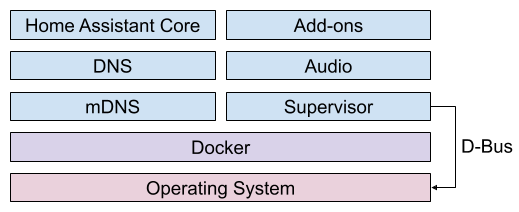
\includegraphics[width=10cm,height=10cm,keepaspectratio]{images/ha_architecture_2020.png}
        \caption{Architektur des Home Assistant Supervisors}
        \label{fig:architectureHAOS}
    \end{figure}
    Die auf dem Supervisor aufbauende Architektur ist die Architektur der Anwendung, der sogenannte Core. Dieser besteht aus vier 
    Komponenten, welche den Hauptteil abbilden: Event Bus, State Machine, Service Registry und Timer\footnote{Entwickler Dokumentation der Home Assistant Plattform. \url{https://developers.home-assistant.io/docs/} Abgerufen am 24.04.2022}. 
    \\
    Mit dem Event Bus wird das Abhören und Auslösen von Events und Ereignisse erleichtert. Die Komponente stellt eine zentrale Eigenschaft 
    der Home Assistant Anwendung dar. Die Zustandsmaschine (State Machine) ist eine weitere Komponente, mit der die Zustände von Dingen, darunter 
    intelligente Geräte, Sensoren uvm., überwacht und Zustandsänderungsereignisse an den Event Bus ausgelöst werden. Dies erfolgt nach der 
    Änderung des Zustandes eines Objektes. Mit der Dienstregistrierung (Service Registry) wird der Event Bus auf eingehende Aufrufe von 
    Diensten abgehört. Über die Service Registry kann der Benutzer Dienste hinzufügen und verwalten. Mittels den Entwicklertools, die über das 
    \ac{UI} aufgerufen werden können, kann der Benutzer die Dienste und Automatisierungen aufrufen und konfigurieren. Das letzte 
    Element, der Timer, ist ebenso eine Komponente der Architektur, die zeitveränderte Ereignisse gemäß einer gegebenen Frequenz 
    an den Event Bus sendet. Somit können zeitbasierte Automatisierungen vereinfacht und ausgelöst werden. Als Datenbank wird eine 
    nicht Cloud-basierte SQLite\footnote{Structured Query Language, eine Datenbanksprache zur Definition, Abfrage und Bearbeitung von Datenstrukturen in relationalen Datenbanken} 
    Datenbank verwendet. Diese ist nur auf dem Gerät enthalten und wird nicht über das Internet übertragen. 
    Im lokalen Netzwerk hat der Nutzer die Möglichkeit, um auf die Datenbank zuzugreifen und eine Historie von Aktionen einzusehen. 
    Eine Verlaufskomponente, die ebenso im Core enthalten ist, speichert die Ereignisse innerhalb der Plattform. Somit können Nutzer auf 
    alle gespeicherten Informationen zu Hause zugreifen und diese einsehen \cite{HAOSarchitecture2018}.
    \\
    \linebreak
    \begin{figure}[hbt!]
        \centering
        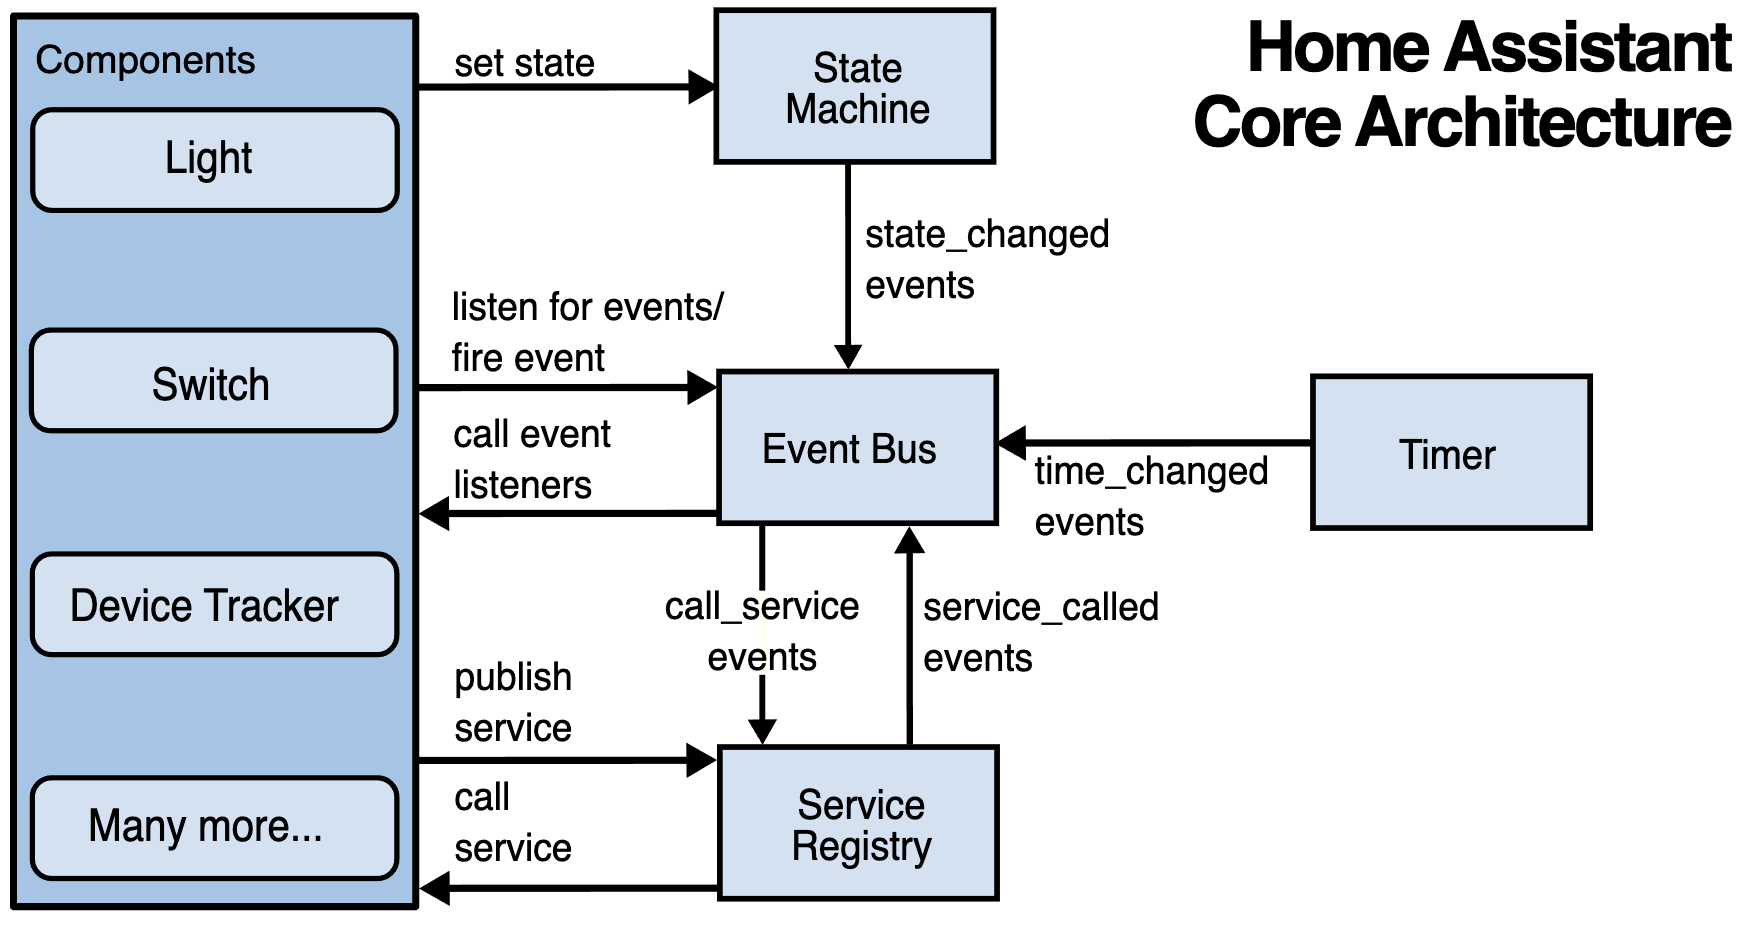
\includegraphics[width=15cm,height=15cm,keepaspectratio]{images/HAOS_Core_Architecture.png}
        \caption{Architektur des Home Assistant Cores \cite{HAOSarchitecture2018}}
        \label{fig:architectureHAOSCore}
    \end{figure}
\subsection{Ziele und Schwerpunkte}
    Jede Softwarelösung verfolgt bestimmte Ziele und Schwerpunkte, damit die Zielerreichung (\ac{DOD}) messbar ist. Die mit 
    der Home Assistant Plattform verfolgten Ziele sind Privatsphäre und Sicherheit, die Wahlmöglichkeiten von Geräten und die Haltbarkeit 
    der Plattform\footnote{Schwerpunkte der Home Assistant Plattform. \url{https://www.home-assistant.io/blog/2021/12/23/the-open-home/} Abgerufen am 24.04.2022}. 
    \\
    \linebreak
    Das Thema der Privatsphäre wird bei Home Assistant dadurch forciert, dass die Geräte nur optional über das Internet erreichbar sind, bzw. 
    nur über das lokale Netzwerk. So kann die Kategorisierung des Verhaltens durch Algorithmen vermieden werden. 
    \\
    Die großflächige Auswahlmöglichkeit von Geräten und Verknüpfungen ist ein weiteres großes Ziel von Home Assistant, da es möglich ist  
    herstellerunabhängig Geräte zu verwenden und zu integrieren. Dadurch können über eine Zentrale mehrere Geräte von diversen Herstellern 
    kombiniert werden.
    \\
    Haltbarkeit wird an der Stelle adressiert, an der die Plattform uneingeschränkt verfügbar ist und Geräte zur Anbindung verwendbar sind. 
    Damit ist auch zu erwarten, dass Geräte, die eingebunden werden können, so konzipiert und gebaut sind, damit sie eine lange Lebensdauer 
    besitzen.
    \\
    \linebreak
    Schwerpunkte, bzw. Lösungen zur Problembehebung sind die Kontrollierbarkeit über eine einzige zentrale Stelle und die Konfiguration von 
    Automationen, die Prozesse selbstständig auslöst. Durch die Möglichkeit der Automatisierung und Steuerung von Komponenten im Eigenheim, 
    bzw. im Büro kann die Lebensqualität erhöht als auch die Energy- und Stromkosten gesenkt werden. Die Kompatibilität der Plattform 
    ermöglicht die Verwendung von mehreren Geräten und Herstellern über eine zentrale Stelle, der Home Assistant Software. Dies ermöglicht 
    dem Nutzer die uneingeschränkte Verwendung von Geräten und die Unabhängigkeit zu Herstellern, die ggf. den Preis der Geräte über dem 
    Marktdurchschnitt verkaufen. Ein weiterer Schwerpunkt ist die Sichtbarkeit der Daten, die potentiell gesendet werden, um den Datenschutz 
    und die Privatsphäre auf dem höchsten Standard zu halten. Ein Auswirkung dafür ist die zugrundeliegende lokale Datenhaltung über die 
    Datenbank, die direkt auf dem Gerät der Plattform läuft.

    %https://apiumhub.com/tech-blog-barcelona/domotics-with-home-assistant-concepts/
    %Home Assistant is created to address these issues:
    %– Could we have a single home automation/control centre, compatible with almost all electronic devices?
    %– Could we make the sending of data to an external server visible? Could we even eliminate it completely?

\subsection{Stärken und Schwächen}
    Die Stärken und Schwächen der Plattform belaufen sich auf die folgenden Aspekte:
    \begin{table}[hbt!]
        \begin{center}
            \begin{tabular}{| p{7.875cm} | p{7.785cm} | }
                \hline
                    \textbf{Stärken} & \textbf{Schwächen} \\
                \hline
                    Open-Source Software & Schwerer Einstieg für neue Nutzer im Hinblick auf die Konfiguration der Automationen \\ 
                \hline
                    Privatsphäre \& Datenschutz & Automationen im YAML-Datenformat und benutzerdefinierte Komponenten können für neue Benutzer schwierig sein \\ 
                \hline
                    Große Community & Langwierige Installationen von Integrationen \\ 
                \hline
                    Automationen sind sehr mächtig & Die Erweiterung, Einrichtung und Konfiguration erfordert die Bearbeitung von YAML-Dateien und einen Neustart bei jeder Änderung \\ 
                \hline
                    Stetige Aktualisierung, Weiterentwicklung und Fehlerbehebung & Automationen können kompliziert aufgebaut sein \\ %  (User Interface zur Erstellung von Automationen wäre für nicht IT-Affine Anwender angebracht.)
                \hline 
                    Unterstützung vieler Geräte (Herstellerunabhängigkeit) und großflächige Kompatibilität & Nutzung von ZigBee und Z-Wave erfordert jeweils eigene Konfigurationen, welche die All-in-One Lösung erschwert. \\
                \hline
                    Individuelle Modifikation der UI &  \\ 
                \hline
                    Kann auf beliebiger Hardware ausgeführt werden &  \\
                \hline
            \end{tabular}
        \end{center}
        \caption{Stärken und Schwächen der Home Assistant Plattform}
        \label{tab:prosConsHAOS}
    \end{table}
    \\
    %Die Auflistung der Punkte geht aus Beiträgen der Community und dokumentierten Erfahrungen der Anwendung. 
    Die Konfiguration von Automationen, Funktionen und Integrationen über YAML-Dateien kann auf der einen Seite als Stärke gewertet werden, 
    da die Syntax flexibel einsetzbar ist und Freiheiten bei der Implementierung bietet und auf der anderen Seite als Schwäche, da die 
    Konfigurationen schnell unübersichtlich werden und anfangs schwer zu verstehen sind. Der Aufwand steigt je nach zu implementierende 
    Funktion und deren Abhängigkeiten zu Geräten und gegebenenfalls zu anderen Prozessen und Automationen. 

\section{openHAB}
\label{sec:openhab}
    Neben der so eben erläuterten Home Assistant Plattform zählt ebenso die openHAB Plattform als bekannt und 
    in der Anwendung populär. Der \ac{OPENHAB} ist eine Plattform, bei der es sich um eine 
    Softwarelösung handelt, die auf Basis der Programmiersprache Java aufgebaut ist. Die Software steht unter 
    der Eclipse Public License und fällt daher unter die Rubrik der Open-Source Software. Durch die Verwendung 
    von Java ist die Anwendung betriebssystemunabhängig und kann auf beliebigen Betriebssystemen laufen. 
    Ähnlich zu der vorgestellten Home Assistant Software, bietet openHAB ebenso User Interfaces die durch 
    den Webbrowser, Android- und iOS-Geräte unterstützt werden. 
    \\
    \linebreak
    In Kombination mit Java wird bei openHAB das \ac{OSGI}-Framework für die Modularität der Software verwendet. Mit Apache 
    Karaf wird ein Container bereitgestellt, der mit Eclipse Equinox als \acs{OSGI} Laufzeitumgebung agiert. Als 
    \acs{HTTP}-Server ist Jetty in Gebrauch. Die einzelnen Frameworks werden nicht im Detail erläutert, lediglich die für das 
    Verständnis des Konzeptes notwendigen.
    \\
    \linebreak
    Mit openHAB wird eine hochmodulare Software zur Verfügung gestellt, die durch sogenannte \textit{Add-ons} erweitert 
    werden kann. Durch diese wird der Plattform eine breite Palette an Funktionen geboten. Physische Geräte können in 
    großer Anzahl mit der Plattform interagieren und verknüpft werden.\footnote{Einleitung zu openHAB. \url{https://www.openhab.org/docs/} Abgerufen am 25.04.2022}

    \subsection*{Historie}
    \label{sec:historyoHAB}
    %TBD...

\subsection{Konzept und Architektur}
%\subsection{Architektur}
    Die Steuerungsplattform openHAB bietet vergleichbar zu Home Assistant die Möglichkeit der multifunktionalen Verknüpfung von 
    Geräten und Protokollen. An dieser Stelle werden ebenso mehrere Konzepte verwendet, die die Vereinheitlichung der Plattform 
    verstärkt. Die Konzepte der openHab Software sind in drei größere Rubriken aufgeteilt, die sich wie folgt zusammensetzen:
    \\
    \linebreak
    Die erste Rubrik sind die Dinge (Things), diese sind die Entitäten, die als physische Komponente zu einem System hinzugefügt 
    und viele Funktionalitäten als eines bereitstellen kann. Hierbei ist zu berücksichtigen, dass die sogenannten Dinge nicht 
    immer Geräte sein müssen, diese können auch andere überschaubare Informationsquellen, andere Webdienste und Funktionalitäten 
    darstellen. Aus Sicht des Benutzers sind sie für den Einrichtungs- und Konfigurationsprozess relevant, für den Betrieb 
    jedoch potentiell zu vernachlässigen. Dinge können Konfigurationseigenschaften haben, die optional oder obligatorisch sein 
    können. Solche Eigenschaften können grundlegende Informationen wie eine IP-Adresse, ein Zugriffstoken für einen Webdienst 
    oder eine gerätespezifische Konfiguration sein, die sein Verhalten ändert \cite{openHAB-article}. Mit dem Konzept der Dinge 
    kommen zwei Unterkategorien einher:
    \begin{itemize}
        \item Kanäle (Channels): Jedes Gerät, bzw. Ding stellt Kanäle bereit, mit denen die jeweiligen Funktionen abgebildet werden. 
        An der Stelle an der das physische Gerät angebunden ist, ist der Kanal eine konkrete Funktion dieser Entität. Beispielsweise 
        kann eine Glühbirne einen Kanal für die Farbtemperatur und einen für den Farbwert besitzen. Diese stellen beide die 
        Funktionalität der einen physischen Glühbirne für das System bereit. Grundlegend sind Kanäle mit Elementen verknüpft, mit denen 
        die virtuelle und physische Ebene verbunden wird. Ab dem Zeitpunkt, sobald eine Verbindung hergestellt wird, reagiert ein Ding 
        auf Ereignisse, die für ein Element transferiert werden. Bedingung dafür ist die Verknüpfung zu einem Kanal. Auf der anderen 
        Seite werden aktiv Ereignisse für Objekte gesendet, die mit Kanälen des Dings verknüpft sind \cite{openHAB-article}.
        \item Brücken (Bridges): Die Brücke ist eine besondere Art von Ding. Diese müssen dem System hinzugefügt werden, damit der 
        Zugriff auf andere Dinge ermöglicht wird, bzw. erhalten bleibt. Ein IP-Gateway für Hausautomationssysteme, welches nicht 
        IP-basiert funktioniert, ist eine typisches Beispiel für so eine Brücke.
    \end{itemize}
    An zweiter Stelle stehen die Artikel (Items). Diese Elemente stellen Funktionen dar, die direkt von der Anwendung verwendet 
    werden. Darunter zählen hauptsächlich die Automatisierungslogik oder auch Benutzeroberflächen. Durch Ereignisse werden die 
    Elemente verwendet, da diese einen Zustand besitzen. 
    \\
    Elemente können auch in eine Gruppe zusammengefasst werden. Ein Gruppenelement kann auch Mitglied einer weiteren Gruppe sein. 
    Diese zyklischen Mitgliedschaften sind war nicht verboten, davon wird jedoch abgeraten. Über Benutzeroberflächen können 
    einzelne Gruppenelemente als alleinstehender Eintrag angezeigt werden und eine Navigation zu den jeweiligen Mitgliedern 
    bereitstellen. 
    \\
    \linebreak
    Die dritte große Rubrik sind die Bindungen und Links (Bindings and Links). Diese können als Softwareadapter betrachtet werden, 
    die Dinge für ihr Hausautomationssystem zur Verfügung stellen \cite{openHAB-article}. Aufgabe der Komponente ist die Verknüpfung 
    von Elementen mit physischen Geräten. Um dies zu ermöglichen werden die spezifischen Kommunikationsanforderungen eines Geräts 
    abstrahiert. Dadurch ist eine allgemeinere Behandlung der Komponente durch das Framework möglich. Links stellen das Bindeglied 
    zwischen Dingen und Gegenständen dar. Es ist die Verknüpfung von genau einem Element und einem Kanal. Elemente und 
    Kanäle haben keine eins zu eins Beziehung zueinander. Eine Verknüpfung mit mehreren Komponenten ist auch hier möglich. 
    \\
    \linebreak
    Die Architektur der openHAB Anwendung %TBD 
    \begin{figure}[hbt!]
        \centering
        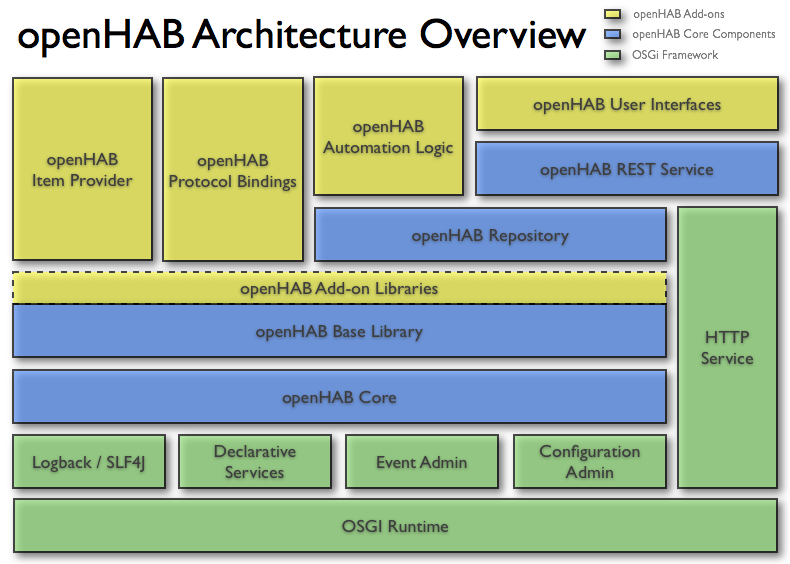
\includegraphics[width=15cm,height=15cm,keepaspectratio]{images/openhab-architecture.png}
        \caption{Architektur der openHAB Plattform \cite{openHAB-architecture2018}}
        \label{fig:architectureopenHAB}
    \end{figure}




\subsection{Ziele und Schwerpunkte}
\subsection{Stärken und Schwächen}

\section{Vergleich von Home Assistant und openHAB}
\label{sec:comparison-HAOS-openHAB}
    %Allgemein gültiger Vergleich (Aufbau, Architektur, Schwerpunkte (Fokus), Umsetzungen, Konnektivität, etc.)
    % https://everythingsmarthome.co.uk/home-assistant-vs-openhab-which-one-is-better/
    % https://smarthome.msuttner.de/openhab-2/vergleich-openhab-vs-home-assistant/ 
    % https://www.electronicshub.org/openhab-vs-home-assistant/ 
    % https://smarthome.university/your-smart-home-platform-home-assistant-vs-openhab/ 


%\section{Requirements Engineering}
\label{sec:requirementsengineering}
    In der heutigen Softwareentwicklung ist zu Anfang jedes Projekts die Frage offen, welche Anforderungen soll das 
    Produkt erfüllen, sodass daraus eine gute, stabil und effiziente Software entsteht und der Umfang und das Ziel 
    klar gestaltet sind. Mit dem \acl{RE} wird der Gedanke verfolgt, die Bedürfnisse des Kunden, bzw. des Stakeholders 
    zu erfüllen und eine erfolgreiche, den Kunden zufriedenstellende Entwicklung des Systems zu erzielen. Ein Stakeholder 
    ist eine Person oder Organisation mit Einfluss auf die Anforderungen des Systems oder die Auswirkungen auf das System 
    hat \cite{pohl2021basiswissen}.
    Diese Anforderungen werden durch das \acl{RE} ermittelt und dokumentiert. 
    \\
    \linebreak
    Unter dem Begriff \ac{RE} ist folgendes zu verstehen: 
    \begin{quote}
        Das Requirements Engineering ist ein systematischer und disziplinierter Ansatz zur Spezifikation und zum 
        Management von Anforderungen mit dem Ziel, die Wünsche und Bedürfnisse der Stakeholder zu verstehen und 
        die Gefahr zu minimieren, ein System auszuliefern, das diese Wünsche und Bedürfnisse nicht erfüllt. \cite{pohl2021basiswissen}
    \end{quote}
    Oft wird darunter auch ein kooperativer und inkrementeller Prozess verstanden, dessen Ziele die Gewährleistung 
    folgender Punkte darstellt:
    \begin{itemize}
        \item Alle Anforderungen sind bekannt und werden auch in dem erforderlichen Detaillierungsgrad verstanden.
        \item Alle involvierten Stakeholder haben eine ausreichende Übereinstimmung über die bekannten Anforderungen erzielt.
        \item Alle Anforderungen sind zu den Dokumentationsvorschriften konform, bzw. zu den Spezifikationsvorschriften konform spezifiziert.
    \end{itemize}
    Damit ist von System-Design, Architekturen oder die nachfolgenden Tests zu differenzieren. 
    \\
    Dieser Prozessschritt deckt die Formalitäten ab, um allen beteiligten eine grundlegende Übersicht zu geben, welche 
    Ziele verfolgt werden, bzw. welche Anforderungen erfüllt werden sollen. Auch ist das \acl{RE} ein wesentlicher 
    Bestandteil des Entwicklungsprozesses nach Scrum. Unter dem Begriff Scrum ist ein Vorgehensmodell zu verstehen, 
    welches zum Projekt- und Produktmanagement in agilen Softwareentwicklungen eingesetzt wird. 
    \\
    \linebreak
    Innerhalb der Anforderungen, die im \acl{RE} ermittelt werden, wird zwischen drei Arten von Anforderungen unterschieden: 
    \begin{itemize}
        \item Funktionale Anforderungen: Diese legen die Funktionalität fest, die durch die Entwicklung des Systems 
            erreicht werden soll. Typischerweise werden diese in Funktions-, Verhaltens- und Strukturanforderungen unterteilt.
        \item Qualitätsanforderungen: Diese legen die Qualitäten des Systems fest und beeinflussen die Gestaltung der 
            Systemarchitektur in größerem Maß als die funktionalen Anforderungen.
        \item Randbedingungen (Constraints): Diese legen die Randbedingungen des Systems fest.
    \end{itemize}
\chapter{Stand der Technik}
Stand der Technik
\section{Theorien}
\section{Methoden}
\section{Techniken}

\chapter{Anforderungsanalyse}
\label{chap:anforderungsanalyse}
    Dieses Kapitel befasst sich im Allgemeinen mit der Anforderungsanalyse und -erhebung. Hierbei wird eine
    Marktanalyse repräsentiert, um das Potential rundum \acl{SH} aufzuzeigen und ein Gefühl 
    dafür zu vermitteln, welche Anforderungen dabei entstehen können, bzw. bereits bestehen. Die Analyse ist 
    mit repräsentativen Statistiken, Studien und Umfragen belegt. Hauptsächlich wird im Rahmen der Anforderungserhebung 
    auf die Methodiken und Techniken eingegangen, die verwendet werden, um 
    Anforderungen zu identifizieren. Diese dienen als Grundlage für die Konzeption der Steuerzentrale. Bestandteile der 
    Anforderungserhebung sind unter anderem zentrale Prozesse des \acl{RE}, ein \textit{user-centered Design}, im Deutschen 
    nutzerzentriertes Design, eine \textit{Target Group Analysis}, im Deutschen Zielgruppenanalyse, und die Durchführung von 
    Experten Interviews. Diese Interviews sind nicht repräsentativ und dienen lediglich der weiträumigeren Informationsgewinnung. 
    \\
    Vorab wird sichergestellt, dass im Rahmen des benutzerzentrierten Designs der Softwareentwickler als Nutzer und Anwender im 
    Vordergrund steht, da dieser die Plattform betreibt, bzw. für die Erweiterung der Software als auch für die 
    Anpassungen auf die eigenen Anwendungsfälle zuständig ist.
    \\
    \linebreak
    Damit ein Eindruck entsteht, welches Marktpotential \acl{SH} Anwendungen haben und welche Anforderungen somit 
    verbunden sind, wird basierend auf gegebenen Studien, Statistiken und Umfragen eine Marktanalyse durchgeführt.

\section{Marktanalyse}
\label{sec:marktanalyse}
    Der Markt rundum \acl{SH} nimmt immer weiter zu. Sei es die Entwicklung von neuen intelligenten Geräten, die 
    Massentauglichkeit von Geräten %, die nicht lange am Markt bestehen 
    oder die stetig wachsende Abdeckung von Anwendungsfällen und Übernahme von Aufgaben und Prozessen. Durch die Vielzahl an 
    Produktanbietern und diversen Kommunikationsmöglichkeiten, ist es schwierig eine Lösung für alle Alternativen und 
    Produktausprägungen anzubieten. Hersteller versuchen mit der angebotenen Produktpalette ihr eigenes Ökosystem im Bereich 
    \acl{SH} zu erstellen, um die Nutzer abhängig zu machen. Der repräsentativen Studie von Deloitte zufolge ist jedoch eine 
    Insellösung bei den Nutzern in Deutschland nicht gefragt \cite{deloitte2018}. Befragt wurden 2000 Konsumenten zwischen 
    19 und 75 Jahren. Einem geringen Anteil von 22 Prozent der 
    Befragten ist die Erweiterbarkeit des Systems mit Produkten anderer Hersteller weniger, bzw. nicht wichtig. Im Gegensatz dazu 
    empfinden 43 Prozent der Befragten die Erweiterbarkeit als wichtig und 28 Prozent als sehr wichtig \cite{deloitte2018}. 
    Demnach müssen die Hersteller eine flexiblere Einsetzbarkeit gewährleisten, damit solche Systeme den Marktdurchbruch 
    erlangen. Dadurch wird die Entwicklung von Plattformen komplexer und umfangreicher. Beispielsweise sind die am weit 
    verbreitetsten Open Source Plattformen, openHAB und Home Assistant, sehr komplex und bilden ein großes Ökosystem ab, da 
    stetig der Zuwachs an integrierbaren Geräten zunimmt und damit der Funktionsumfang steigt.  

    \subsection{Allgemeine Marktsituation und Marktprognose}
    %Anbieter, Plattformen, Geräte
        Derzeit gibt es viele Anbieter für intelligente Produkte. Diese bieten zum einen einzelne Geräte an, die in 
        beliebige Plattformen integriert werden können und zum anderen ein eigenes Ökosystem, sofern der Anwender 
        mehrere Produkte des Anbieters nutzen möchte. Dennoch ist in den meisten Fällen die Konfiguration der Geräte nur auf 
        den hauseigenen Plattformen möglich. Somit kann der Nutzer nicht alle Komponenten ausschließlich über eine Plattform 
        konfigurieren und steuern. 
        \\
        \linebreak
        Eine repräsentative Umfrage der \ac{SGCS} mit 1384 Teilnehmern, welche im April 2022 veröffentlicht wurde, zeigt, welche 
        Anbieter in Deutschland am meist verbreitetsten sind, bzw. welche die Nutzer am häufigsten kaufen. An oberster Stelle 
        steht Philips und Samsung mit jeweils 25 Prozent und an dritter Stelle Bosch mit 23 Prozent. Weitere Anbieter können dem 
        Diagramm im Anhang (siehe \ref{appendix:brandings}) entnommen werden. Dabei sind jedoch weitaus nicht alle Hersteller und 
        Anbieter aufgelistet. Detaillierter wird an dieser Stelle jedoch nicht eingegangen. 
        \\
        \linebreak
        Der aktuelle Markt für intelligente Produkte ist in sechs primäre Segmente aufgeteilt, die jeweils andere Anwendungsfälle 
        abdecken \cite{statista2021}:
        \begin{itemize}
            \item Kontrolle und Konnektivität: Gateways die alle Geräte jeglicher Segmente kontrollieren, intelligente Lautsprecher 
            mit dem Fokus zur Kontrolle und der digitalen Unterstützung und bspw. intelligente Steckdosen
            \item Intelligente Geräte (Smart Appliances): Kühlschrank, Waschmaschine und Geschirrspüler, Kaffeemaschine, Mikrowelle 
            und Staubsaugerroboter
            \item Sicherheit: Bewegungs-, Wasser- und Rauchmelder, Kameras und Türschlösser
            \item Heimunterhaltung (Home Entertainment): Fernseher, Entertainment-Systeme 
            \item Komfort und Licht: Intelligente LEDs, Fenster- und Tür-Sensoren etc.
            \item Energiemanagement: Thermostate und Regler, Luftqualitätsmesser etc. 
        \end{itemize}
        \pagebreak
        Die aufgelisteten Segmente werden von vielen Herstellern bedient. Darunter sind der folgenden Abbildung die 
        repräsentativen Schlüsselanbieter zu entnehmen:
        \begin{figure}[hbt!]
            \centering
            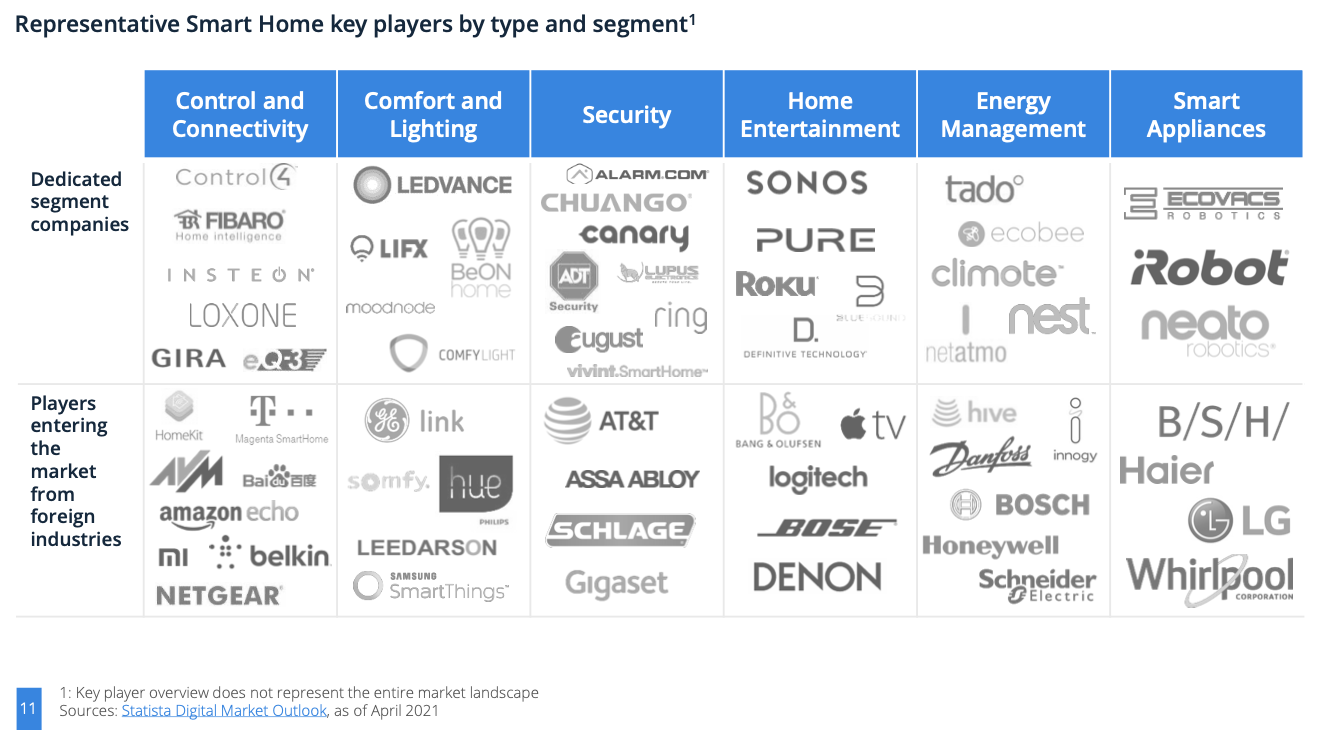
\includegraphics[width=15cm,height=10cm,keepaspectratio]{images/keyplayers.png}
            \caption{Übersicht der repräsentativen Schlüsselanbieter \cite{statista2021}} 
            \label{pic:landscape}
        \end{figure}
        \\
        Die Übersicht deckt jedoch nicht alle Anbieter ab und spezialisiert sich in diesem Fall auf die bekanntesten und die am 
        Markt etablierten. 
        \\
        \linebreak
        Laut den von Statista veröffentlichten Daten war die USA mit einem Umsatz von 28,86 Milliarden US-Dollar der größte 
        \acl{SH} Markt im Jahr 2021, wogegen Deutschland eine Umsatz von 6,59 Milliarden US-Dollar erzielte. Zu berücksichtigen sind 
        dabei jedoch die Demographische Lage als auch die Bevölkerungsdichte. Diese Aufstellung steht in keinem direkten Vergleich und 
        dient lediglich zur Veranschaulichung und zur Unterscheidung der Marktanteile. Deutlich wird dabei jedoch, dass das 
        Marktwachstum prozentual ähnlich ansteigt. 
        \\
        \linebreak
        Der Markt-Prognose in Abbildung (\ref{pic:revenue}) ist zu entnehmen, dass bis 2026 sich der Umsatz nahezu verdoppeln 
        wird. Der Darstellung (\ref{pic:globalmarket}) der einzelnen Segmente kann entnommen werden, dass der Weltmarkt von 
        2021 bis 2026 um ca. 100 Prozent zunimmt. Die Zeitspanne von 2019 bis 2026 stellt einen durchschnittlichen Zuwachs von 
        17,4 Prozent dar. Anhand der Prognose und des Berichts von Statista ist deutlich zu sehen, dass der \acl{SH} Markt in 
        den nächsten Jahren erheblich wachsen wird. Prognostiziert ist ein globaler Marktwert bei ca. 207,8 Milliarden 
        US-Dollar bis 2026.
        \begin{figure}[hbt!]
            \centering
            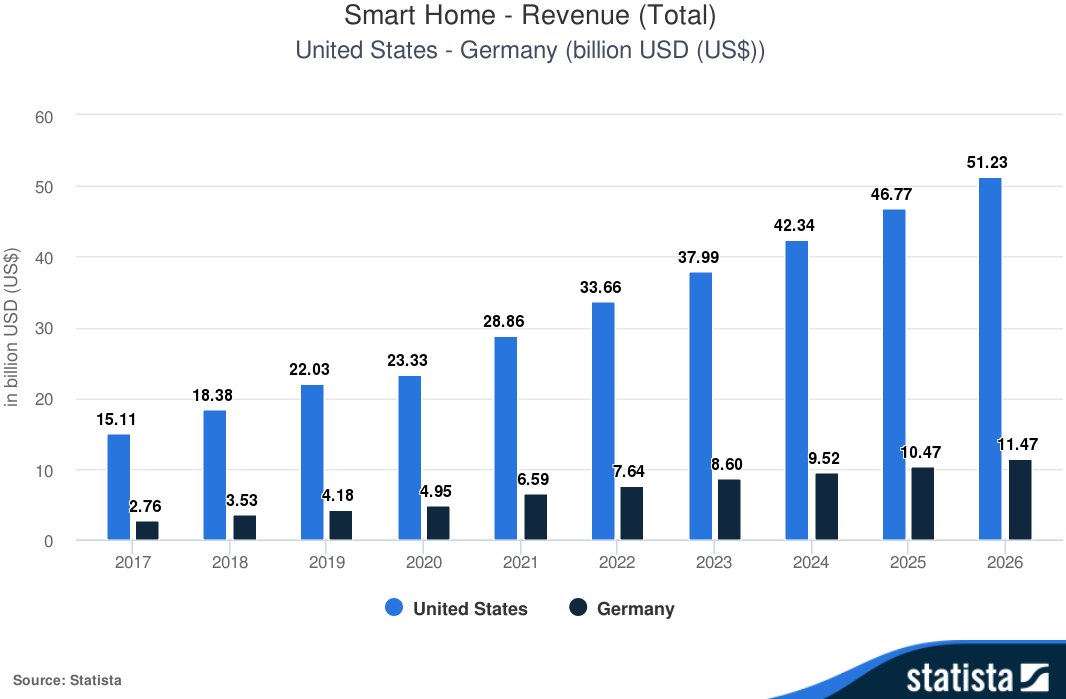
\includegraphics[width=15cm,height=9.25cm,keepaspectratio]{images/Statista-Outlook-Smart-Home---Revenue-Total-United-States---Germany-billion-USD-US.png}
            \caption{Umsatz-Prognose von Deutschland und den USA \cite{statista2021}} 
            \label{pic:revenue}
        \end{figure}
        \\
        \begin{figure}[hbt!]
            \centering
            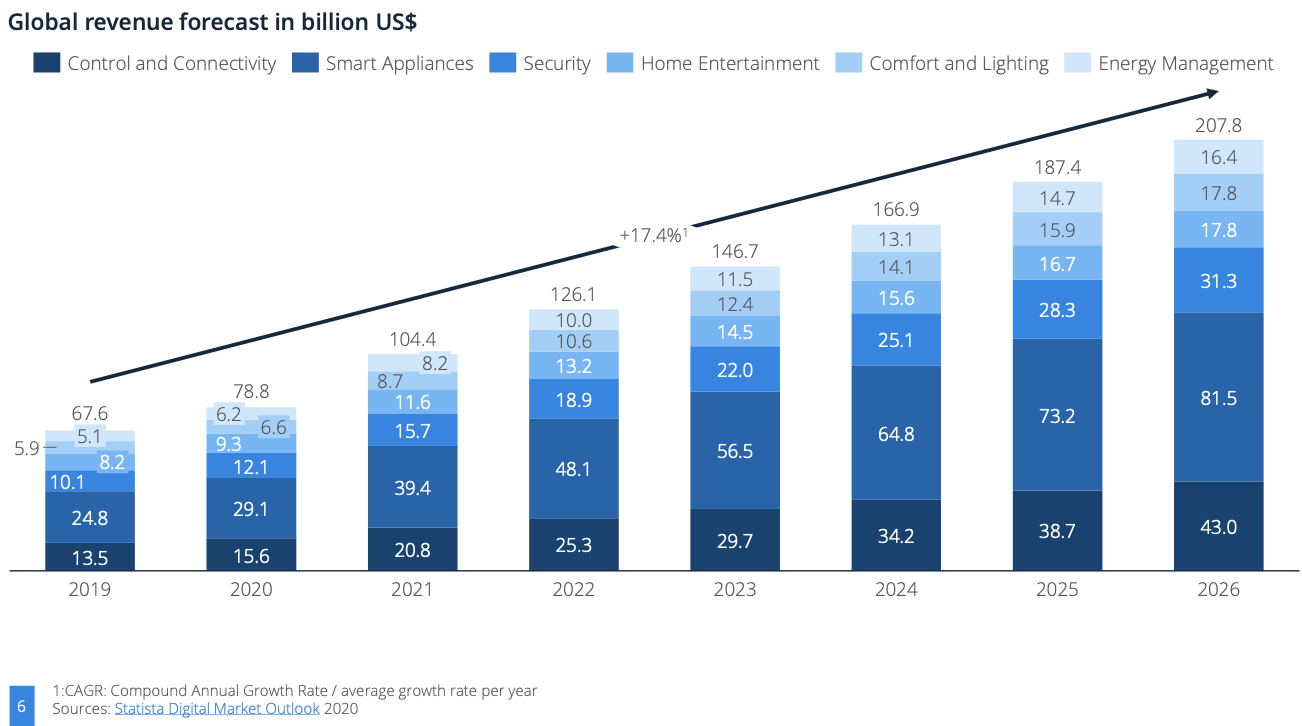
\includegraphics[width=15cm,height=10cm,keepaspectratio]{images/global_Worth_smart-home.png}
            \caption{Globaler Smart Home Marktwert \cite{statista2021}} 
            \label{pic:globalmarket}
        \end{figure}
        \pagebreak 
    \subsection*{Schlüsseltechnologien und Barrieren}
        Unter den Schlüsseltechnologien im \acl{SH} sind Komponenten zu verstehen, die den Gedanken eines intelligenten 
        Wohnraumes und Gebäudes forcieren. Dazu zählen unter anderem die Spracherkennung, die bei Sprachassistenten, 
        darunter bspw. Amazon Alexa, Apple HomePod (Siri) und dem Google Nest, eingesetzt wird, sowie \ac{AI} und \ac{KI} 
        zur Analyse, Auswertung und Optimierung von Verhaltensmustern und weiteren Analysezwecken \cite{statista2021}. 
        Obwohl die Spracherkennung das Wachstum des Marktes ankurbelt, werden die herkömmlichen Interaktionsmöglichkeiten, 
        z.B. die Kontrolle über Berührung durch Touch-Displays,
        weiter bestehen und weiterhin eine wichtige Art des Gerätezugriffs darstellen \cite{all-electronics2022}. 
        Mit dem Einsatz von \acs{KI} und \acs{AI} werden Prozesse noch autonomer und können den Komfort aus den Analysen je 
        nach Bedürfnis individuell gestalten. Zu berücksichtigen ist dabei jedoch die dafür geeigneten Anwendungsfälle und 
        die Bereitschaft der Nutzer, in wie fern diese das Analysieren von Verhaltensmustern akzeptieren und zulassen. 
            
        \subsubsection*{Fehlender Interoperabilität}
            Die Kommunikation von \acl{SH} Geräten findet über drahtlose Netzwerke auf Brandbreiten statt, die oft nicht 
            miteinander kompatibel sind. Der hauptsächliche Grund dafür ist, dass Unternehmen ein Protokoll für einen 
            bestimmten Zweck entwickeln und dieses darauf abgestimmt ist den Anwendungsfall abzudecken und um eine 
            Markteintrittsbarriere zu schaffen, sodass der Wechsel zwischen Anbietern erschwert wird \cite{statista2021}. 
            Die damit einhergehende Schwachstelle eines \acl{SH} ist, dass die Geräte mit den bereits entwickelten 
            Protokollen genutzt werden. So ist die Kommunikation über verschiedene Protokollen nicht vorgesehen. Dadurch 
            entsteht die fehlende Interoperabilität, die der Anwender jedoch für eine \acl{SH} Lösung ansieht und auch 
            als äußerst sinnvoll betrachtet. Die Einführung von Bluetooth LE Mesh ist eine aktuelle Entwicklung, um der 
            Herausforderung der Bewältigung der Interoperabilität einen Schritt näher zu kommen. Dennoch muss der 
            Anwender prüfen, welche Geräte miteinander kompatibel sind \cite{statista2021}. Bei cloudbasierten 
            Sprachdiensten muss ebenso die Kompatibilität geprüft werden. 
            Dadurch wird dem Nutzer neben der Ungewissheit der Datensicherheit und der Privatsphäre ein weiterer Aspekt 
            geliefert, der die Nutzung von \acl{SH} Lösungen für bestimmte Anwendergruppen immer noch in Frage stellt.
            \\ 
            \linebreak
            Derzeit häufig verwendete Protokolle sind unter anderem Bluetooth, \ac{WLAN} (WiFi), KNX, ZigBee, Z-Wave, 
            MQTT und weitere (siehe \ref{tab:protocolsSH}). Um Beispielsweise mit ZigBee über \acs{MQTT} kommunizieren zu 
            können, gibt es ein Framework, welches die Interoperabilität der beiden Protokolle ermöglicht. Dies ist das 
            sogenannte \textit{ZigBee2MQTT} Framework\footnote{Erschafft eine Brücke zwischen ZigBEE und MQTT. \url{https://www.zigbee2mqtt.io/} Abgerufen am 23.05.2022}.
\pagebreak
\section{Zielgruppenanalyse}
\label{sec:zielgruppenanalyse}
    Zur Analyse der Zielgruppen, die \acl{SH} Lösungen nutzen, bzw. die als Anwender des im Rahmen dieser Arbeit 
    entstehenden Konzeptes gelten, erfolgt in diesem Abschnitt eine Zielgruppenanalyse. Hierbei wird zwischen 
    zwei Gruppen stark differenziert. Zum einen erfolgt die Benutzer-Analyse, die aufzeigt, welche Zielgruppen 
    im allgemeinen Kontext \acl{SH} adressiert werden, und zum anderen die Anwender-Analyse, die sich 
    konkret der Zielgruppe widmet, die in dieser Arbeit adressiert wird. 

    \subsection{Ziel der Zielgruppenanalyse}
        %was soll damit erzielt werden?
        Ziel einer Zielgruppenanalyse\footnote{Beschreibung der Zielgruppenanalyse und mögliche Durchführungsschritte. \url{https://www.eology.net/magazine/target-group-analysis} Abgerufen am 24.05.2022.} 
        ist die Identifizierung der Personengruppen, die als potentielle Nutzer eines Produktes 
        oder eines Marktsegmentes gelten. Diese Methodik ist ein relevantes Werkzeug in der Produktkonzeption und -entwicklung 
        als auch in der Marktforschung. Maßnahmen und Anforderungen können aus der Zielgruppenanalyse abgeleitet und 
        erarbeitet werden. 
        \\
        Ein Weiteres Ziel ist das bessere Kennenlernen der Zielgruppe, um dadurch deren Bedürfnisse und Interessen 
        genauer zu identifizieren und zu betrachten. 
    
        \subsection{Benutzer-Zielgruppe}
        % Smart Home - Deutschland. Zugriff: 11. Mai 2022. https://de.statista.com/outlook/dmo/smart-home/deutschland
            Die in der Marktanalyse (\ref{sec:marktanalyse}) identifizierten Segmente werden in der Abbildung 
            (\ref{pic:segments}) nochmals aufgegriffen. Hierbei wird in der repräsentativen Statistik und Prognose der 
            Statista GmbH die Nutzung des jeweiligen Segments veranschaulicht. Der Fokus dieser Prognose liegt 
            auf der verstärkten Vertretung eines Segments in einem \acl{SH} in Deutschland. Die derzeit am meisten eingesetzten 
            Segmente sind \textit{Vernetzung und Steuerung} (rot gekennzeichnet) und \textit{Komfort und Licht} 
            (gelb gekennzeichnet). Das am wenigsten genutzt Segment stellt die \textit{Gebäudesicherheit} 
            (schwarz gekennzeichnet) in der Prognose dar. Im Jahr 2021 lag die Nutzung von Geräten des Segments \textit{Vernetzung 
            und Steuerung} bei 6,6 Millionen Nutzer, dicht gefolgt von dem Segment \textit{Komfort und Licht} mit 
            6,5 Millionen Nutzer. Dagegen liegt das Segment \textit{Home Entertainment} im Jahr 2021 bei 3,8 Millionen Nutzer.
            \\
            \linebreak
            Die bis 2026 veröffentlichte Prognose gibt vor, dass die jeweiligen Segmente stark zunehmen %werden 
            und sich jeweils vervierfachen.  
            \pagebreak
            \begin{figure}[hbt!]
                \centering
                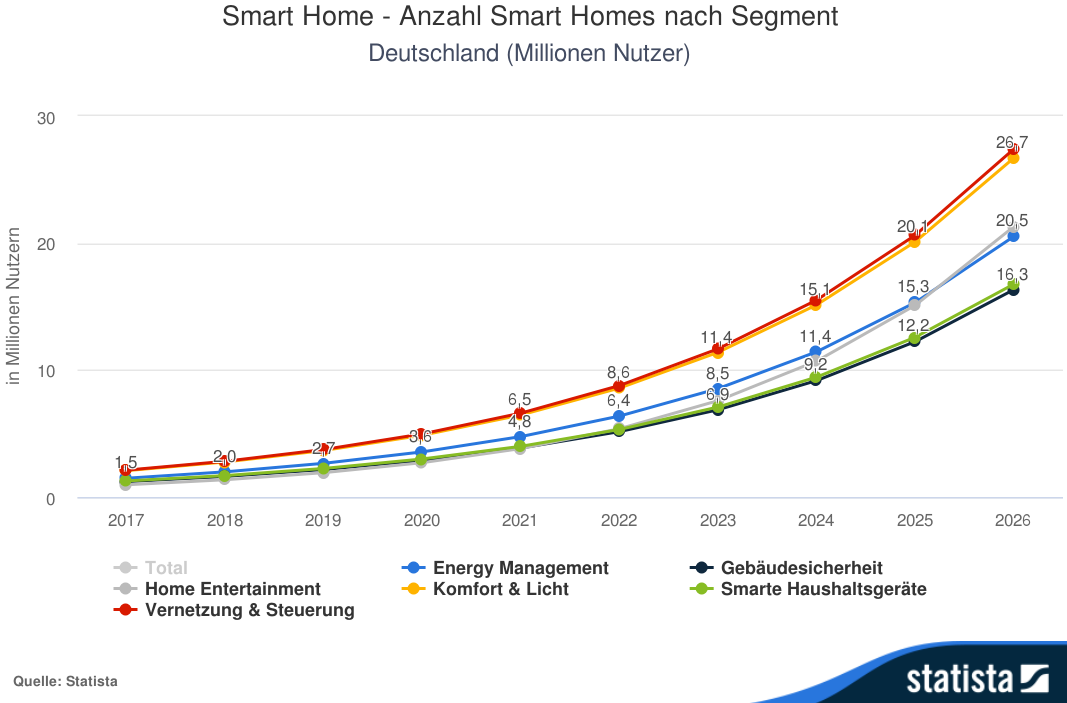
\includegraphics[width=15cm,height=10cm,keepaspectratio]{images/Statista-Outlook-Smart-Home---Anzahl-Smart-Homes-nach-Segment-Deutschland-Millionen-Nutzer.png}
                \caption{Anzahl Smart Home nach Segment \cite{statista2021}} 
                \label{pic:segments}
            \end{figure}
            \\
            Das Resümee der Prognose zeigt, dass eine breitere Masse an Personen bereits Komponenten der Segmente 
            \textit{Vernetzung und Steuerung} und \textit{Komfort und Licht} nutzen.
            \\
            \linebreak
            Im Hinblick auf die demographischen Statistiken wird in der Zielgruppenanalyse deutlich, welche Gesellschaftsschicht 
            im Jahr 2021 am stärksten vertreten ist. Diese erstreckt sich über eine Altersspanne von 25 bis 54 Jahren. 
            Wobei der Abbildung (\ref{pic:ageSH}) zu entnehmen ist, dass der Schwerpunkte im Alter zwischen 45 und 54 Jahren 
            mit 22,7 Prozent. Die Balance nach Geschlecht liegt bei einem Anteil von 45,6 Prozent weiblichen Befragten und 
            54,4 Prozent männlichen Befragten, demnach eine geringe Ungleichheit. Die Auswertung nach Einkommen zeigt, dass 
            35,4 Prozent der Befragten mit mittlerem Einkommen Komponenten eines \acl{SH} nutzen, dicht gefolgt von 
            Personen mit hohem Einkommen, diese liegen bei 34,9 Prozent. 
            \\
            \linebreak
            Demzufolge ist eine große Masse adressiert, die jedoch nach den Segmenten (siehe Abbildung \ref{pic:segments}) 
            wiederum eingeschränkt werden kann.
            \begin{figure}[hbt!]
                \centering
                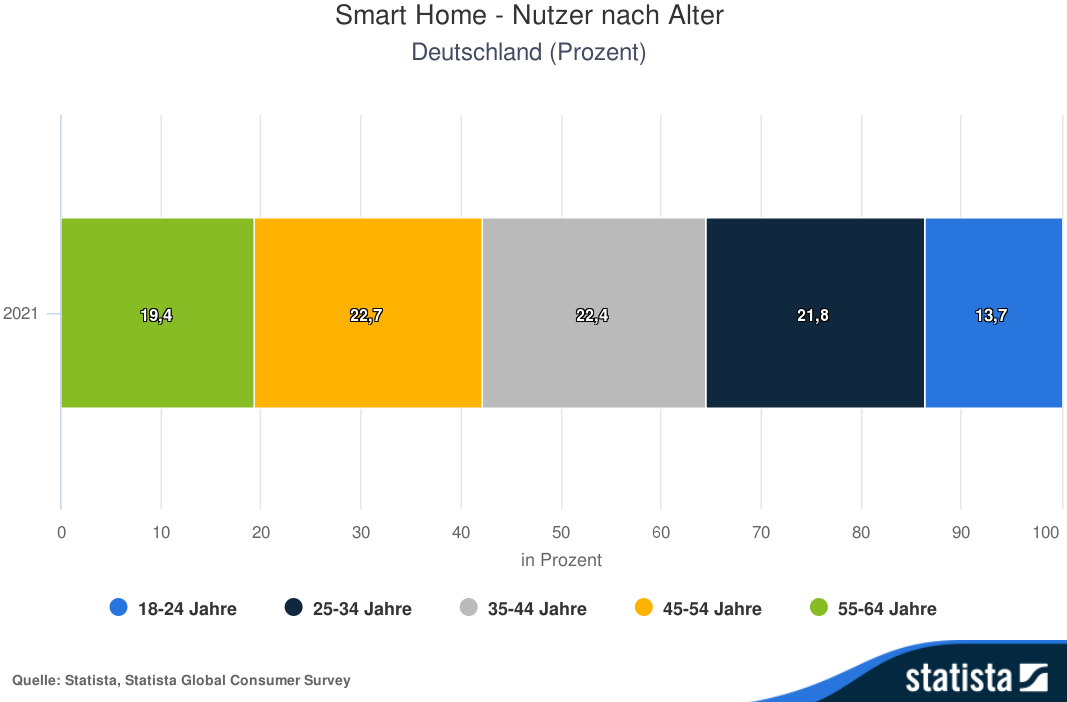
\includegraphics[width=15cm,height=10cm,keepaspectratio]{images/Statista-Outlook-Smart-Home---Nutzer-nach-Alter-Deutschland-Prozent.png}
                \caption{Smart Home Nutzer nach Alter \cite{statista2021}} 
                \label{pic:ageSH}
            \end{figure}
            Die aufgeführten Statistiken und Prognosen zeigen den Markt rundum \acl{SH} auf und welches Potential für die 
            nächsten Jahre prognostiziert wird. Im Hinblick auf die Zielgruppe lässt sich sagen, dass eine breite Masse 
            fokussiert werden kann, die jeweils unterschiedliche Voraussetzungen und Bedürfnisse haben. Diese Analyse zeigt 
            jedoch den gesamten Markt auf, um einen Einblick zu gewährleisten, wie stark \acl{SH} momentan in Deutschland, den 
            Vereinigten Staaten (USA) und dem Rest der Welt vertreten ist. Um einen konkreteren Einblick 
            zu gelangen, wird in nachfolgendem Abschnitt auf die Zielgruppe der Anwender, die in dieser Arbeit fokussiert werden, 
            eingegangen. 

        \subsection{Anwender-Zielgruppe}
            Der Benutzergruppe wird die Anwenderzielgruppe gegenübergestellt, diese können jedoch ebenso Benutzer der Anwendung 
            werden. Im Umkehrschluss ist ein gewisses Maß an \acs{IT}-Affinität vorausgesetzt, sodass Benutzer nicht gleich Anwender 
            sind. Es wird eine grundlegende Kenntnis der Programmierung erfordert, im Rahmen dieser Arbeit der Umgang mit der 
            Programmiersprache Java. 
            \\
            Im Fokus steht der Softwareentwickler als Anwender, welcher das System betreibt und auf die individuellen Bedürfnisse 
            anpasst. 
            %Die eigentliche Zielgruppe, die
        %Softwareentwickler, die das System betreiben und für ihre Bedürfnisse anpassen.

\section{Use Cases}
\label{sec:usecases}
    Für die Erhebung und Ausarbeitung aller Anforderungen an das System, werden Anwendungsfälle, sogenannte Use Cases, 
    definiert, bewertet und auf ihre Funktionalität geprüft und dokumentiert. Zum besseren Verständnis wird auf diese in den 
    folgenden Abschnitten eingegangen. 
\subsection{Check in mit Temi}
\subsection{Notfallevakuierung mit Temi}
\section{Experten Interview}
\label{sec:experteninterviewReqirements}
    Zur Analyse und Erhebung von Anforderungen, die sich an das System richten, werden Experten Interviews durchgeführt. 
    Dabei wird sich, wie in dem Abschnitt (\ref{subsec:experteninterview}) beschrieben, an dem unstrukturierten Ansatz der 
    Führung eines solchen Interviews orientiert \cite{robson2002real}. Infolgedessen werden keine konkreten offenen oder 
    geschlossenen Fragen gestellt. Auf den Aufbau des Interviews wird in weiteren Schritten eingegangen. 
    \\
    Diese Interviews sind nicht repräsentativ, da sie im Rahmen dieser Arbeit keine große Masse abdecken. Diese dienen 
    lediglich der weiträumigeren Informationsgewinnung und dem Sammeln mehrerer Meinungsbilder, um aus allen Ideen, 
    Gedankenanstößen und Meinungen ein objektives Ergebnis und viele Anforderungen zu erhalten. 
    %Die Experten Interviews sind eine Möglichkeit, die Anforderungen zu erfassen, die durch die Entwicklung des Systems 
    %nicht durch eine einfache Marktanalyse erfasst werden konnten. Diese Interviews sind nicht repräsentativ und dienen lediglich 
    %der weiträumigeren Informationsgewinnung.
\subsection{Ziele des Experten Interviews}
    % Diese helfen dabei, mehrere Sichten, Meinungen und Erfahrungen einzuholen, um ein 

\subsection{Aufbau des Experten Interviews}
\subsection{Zusammenfassung der Experten Interviews}
    % Aus den Interviews ergaben sich Anforderungen, die in die Konzeption mit einfließen. Diese werden im folgenden 
    % Abschnitt thematisiert.
\section{Anforderungen}

\begin{landscape}
  \AddToShipoutPictureBG*{%
  \AtPageLowerLeft{%
    \raisebox{\dimexpr.5\paperheight-.5\height}{%
      \makebox[.9\paperwidth][r]{%
        \rotatebox{90}
        {\thepage}
      }% \makebox
    }% \raisebox
  }% \AtPageCenter
}% \AddToShipoutPictureBG*
  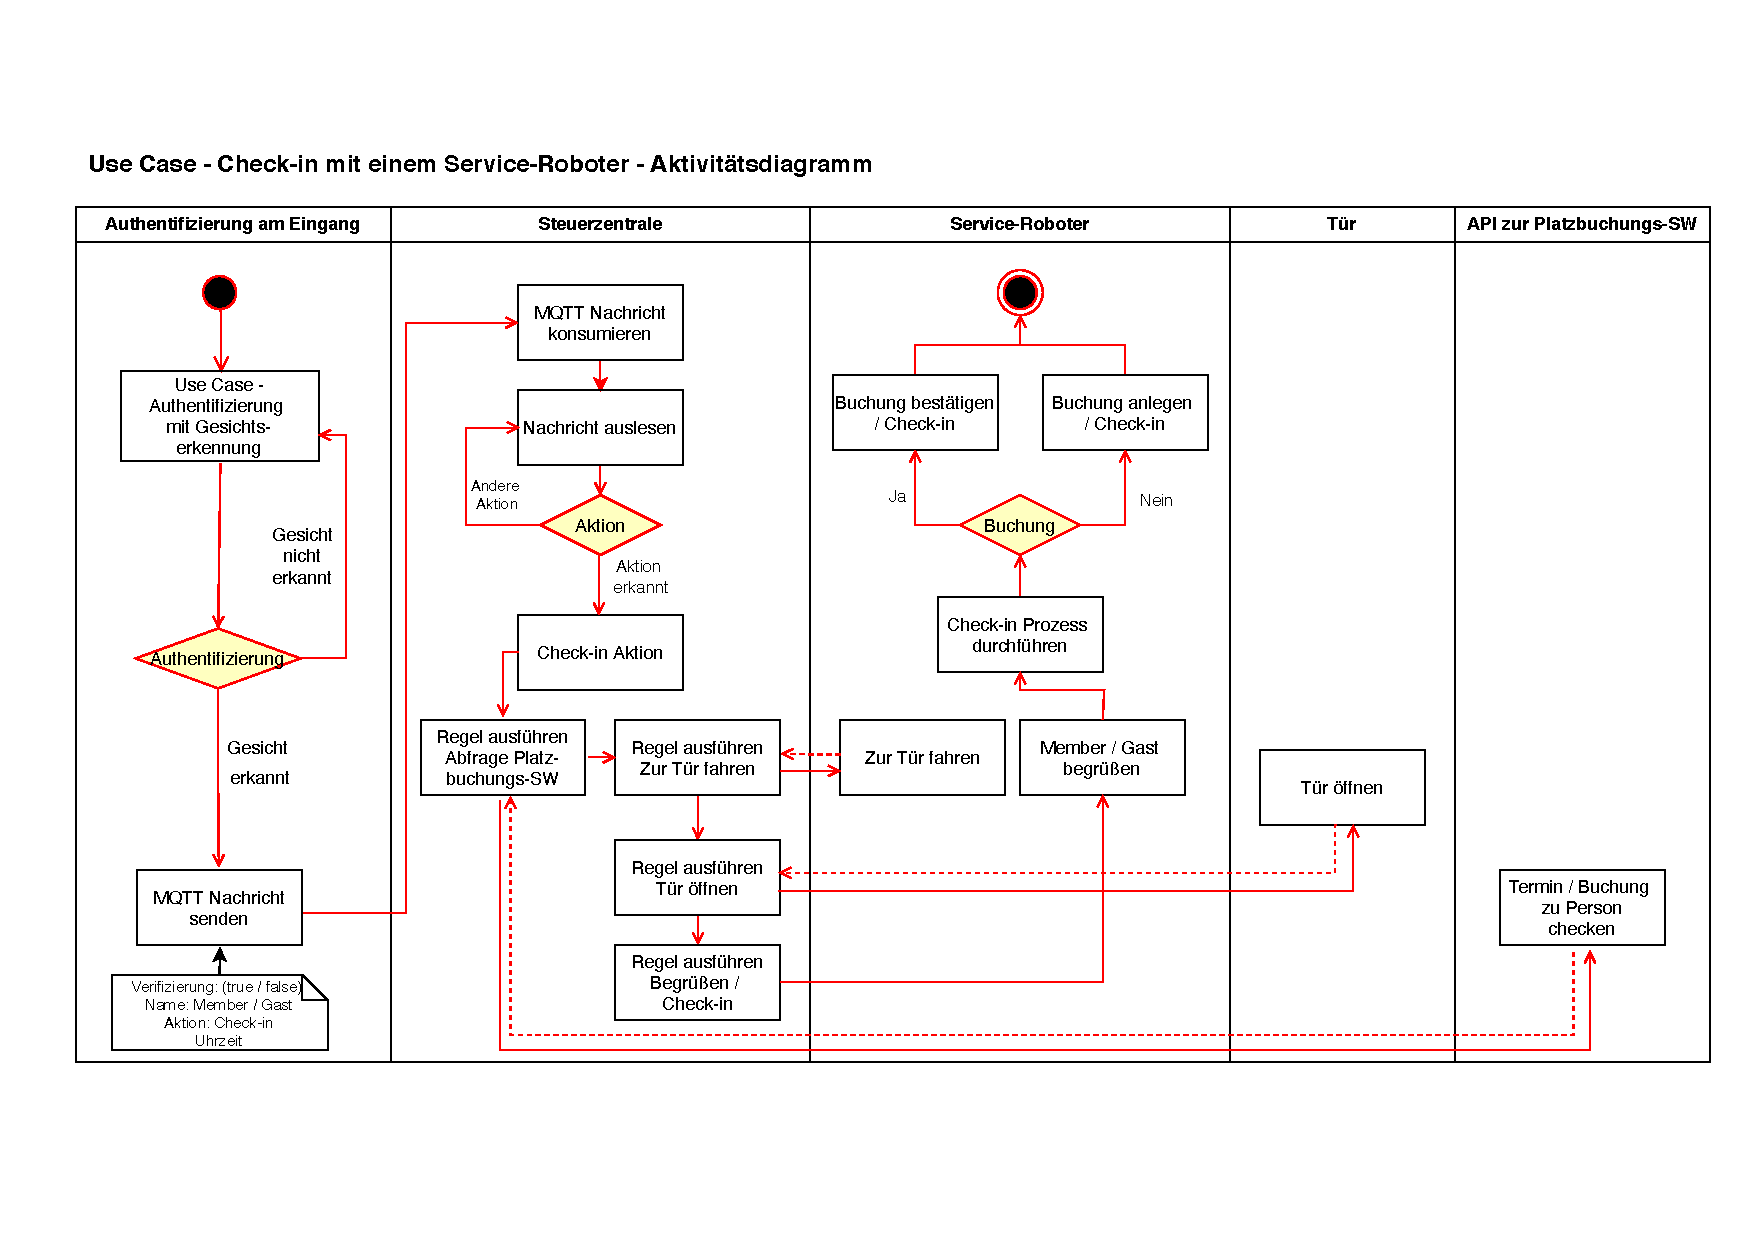
\includepdf[scale=0.75, pages=-, angle=90, fitpaper=true, ]{images/UC1_Aktionsdiagramm_Check-in.pdf}
\end{landscape}
\begin{landscape}
  \AddToShipoutPictureBG*{%
  \AtPageLowerLeft{%
    \raisebox{\dimexpr.5\paperheight-.5\height}{%
      \makebox[.9\paperwidth][r]{%
        \rotatebox{90}
        {\thepage}
      }% \makebox
    }% \raisebox
  }% \AtPageCenter
}% \AddToShipoutPictureBG*
  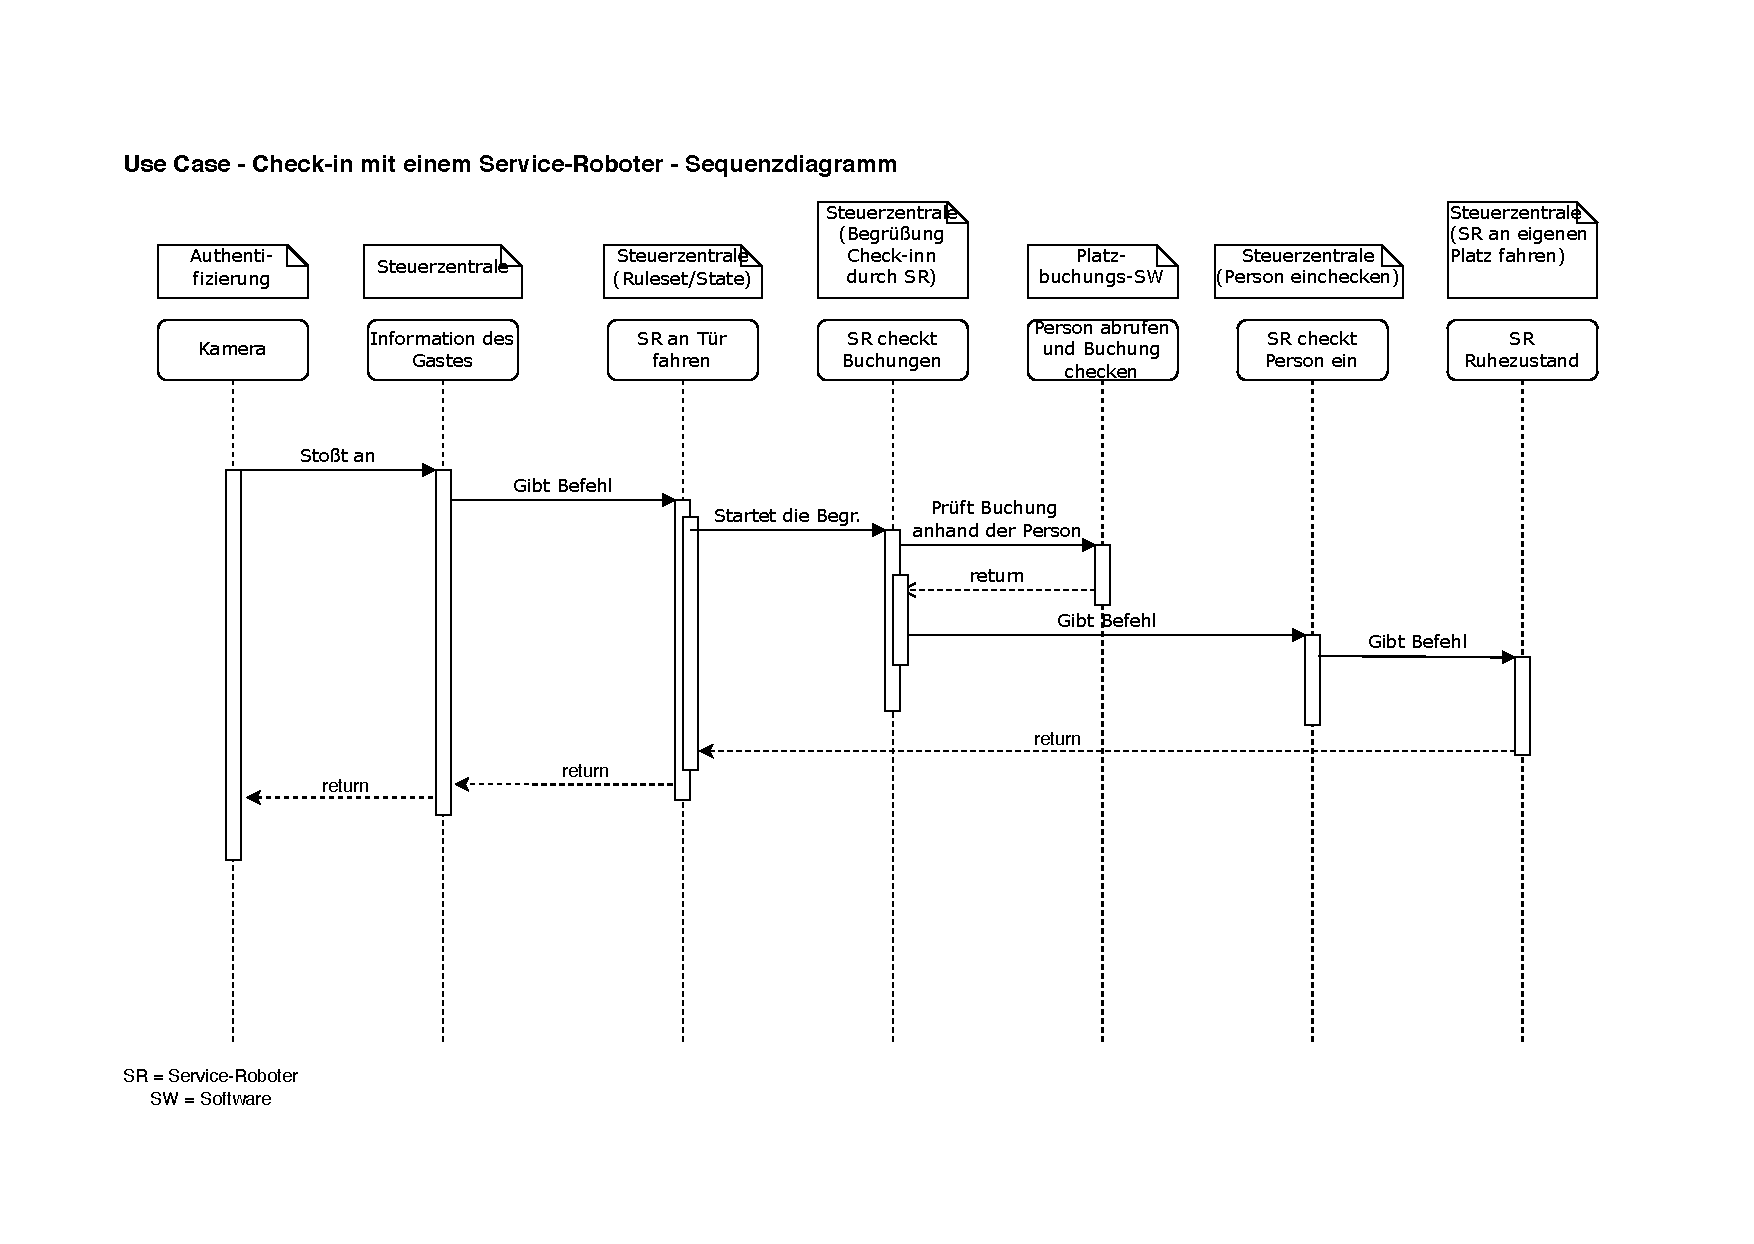
\includepdf[scale=0.75, pages=-, angle=90, fitpaper=true, ]{images/UC1_Sequenzdiagramm_Check-in.pdf}
\end{landscape}
\subsection{Notfall-Evakuierung mit einem Service-Roboter}
\label{subsec:evacuation}
    Mit dem Szenario der Notfall-Evakuierung wird ein weiterer Anwendungsfall definiert, welcher dabei helfen soll, die 
    Anforderungen zu identifizieren, die für die Bereitstellung des Frameworks der Steuerzentrale benötigt werden.
    \\
    \linebreak
    Objektiv betrachtet gibt es bei diesem Fall ebenso einen Auslöser, bspw. einen Rauch- 
    oder Gasmelder, der eine \acs{MQTT}-Nachricht veröffentlicht, die über die Steuerzentrale konsumiert, verarbeitet und dadurch die 
    weiteren notwendigen Schritte eingeleitet werden. Nachdem das \acs{MQTT}-Topic mit der Nachricht von der Steuerzentrale erhalten wurde, wird 
    basierend auf dem Nachrichteninhalt die Regel und die darauffolgende Aktion angestoßen. Die Steuerzentrale muss über die \acs{API} 
    Schnittstelle des internen Büroplatzbuchungssystems alle eingecheckten Personen und Platzbuchungen abfragen und 
    zwischenspeichern. Die Informationen werden genutzt, um den Service-Roboter an die Arbeitsplätze der jeweilig 
    eingecheckten Personen zu schicken, sodass dadurch diese über den Notfall informiert, bzw. gebeten werden, das 
    Gebäude zu verlassen. Wird eine Person an einem Arbeitsplatz erkannt, so kann diese über den Sachverhalt informiert 
    werden. Ist jedoch der Arbeitsplatz leer, soll der Service-Roboter den nächsten Arbeitsplatz ansteuern. Nachdem alle 
    Plätze von dem Service-Roboter abgefahren wurden, soll dieser über die restliche Bürofläche fahren und nach Personen 
    Ausschau halten. Die Erkennung der Person wird durch die Kamera des Roboters durchgeführt. Abschließend, wenn alle Plätze und die 
    Bürofläche abgefahren wurden, soll der Roboter an eine zentrale Stelle im Büro fahren und ohne Unterbrechung eine 
    Durchsage starten und diese solange wiederholen, bis eine Person den Vorgang manuell beendet. Mit der Beendung der Dauerschleife 
    ist das Szenario abgeschlossen und der Roboter kann an seine Ausgangsposition zurückgeführt werden, sofern dies 
    umgebungsbedingt noch möglich ist. Die grobe Skizzierung ist folgendem Anwendungsfalldiagramm zu entnehmen: 
    \begin{figure}[hbt!]
        \centering
        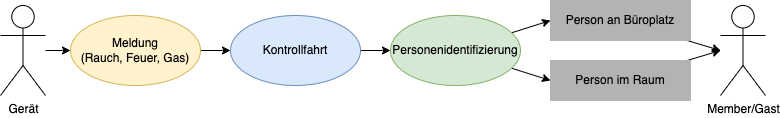
\includegraphics[width=15cm,height=15cm,keepaspectratio]{images/UC2_Diagramm_Notfall.png}
        \caption{Use Case 2 - Anwendungsfalldiagramm}
        \label{fig:uc2-emergency}
    \end{figure}
    \\
    %\linebreak
    Die Anwendungsfälle wurden so gewählt, da diese eine gewisse Komplexität mit sich bringen, die es mit der Steuerzentrale 
    abzudecken gilt.
    \\
    \linebreak
    Zur Stützung der textuellen Schilderung des zweiten Anwendungsfalls werden nachfolgend Diagramme dargestellt, die das Szenarien 
    widerspiegeln. Im Rahmen des \acs{RE} wurden hierfür ebenso eine konkrete Aufgabenbeschreibung, sowie eine User Story und ein Ablaufdiagramm definiert. Diese sind dem 
    Anhang (siehe Anhang \ref{appendix:user-story-uc2}) zu entnehmen. Die folgenden Abbildungen stellen sich aus einem 
    Aktivitätsdiagramm und einem Sequenzdiagramm zusammen: %und einem Ablaufdiagramm zusammen: 
    %\\
    %Aus dem Kontext beider Anwendungsfälle, der vorangestellten Zielgruppenanalyse und den Experteninterviews werden in Abschnitt 
    %(\ref{sec:requirementsFinal}) die daraus identifizierten Anforderungen für die Steuerzentrale aufgeführt.
    
\begin{landscape}
  \AddToShipoutPictureBG*{%
  \AtPageLowerLeft{%
    \raisebox{\dimexpr.5\paperheight-.5\height}{%
      \makebox[.9\paperwidth][r]{%
        \rotatebox{90}
        {\thepage}
      }% \makebox
    }% \raisebox
  }% \AtPageCenter
}% \AddToShipoutPictureBG*
  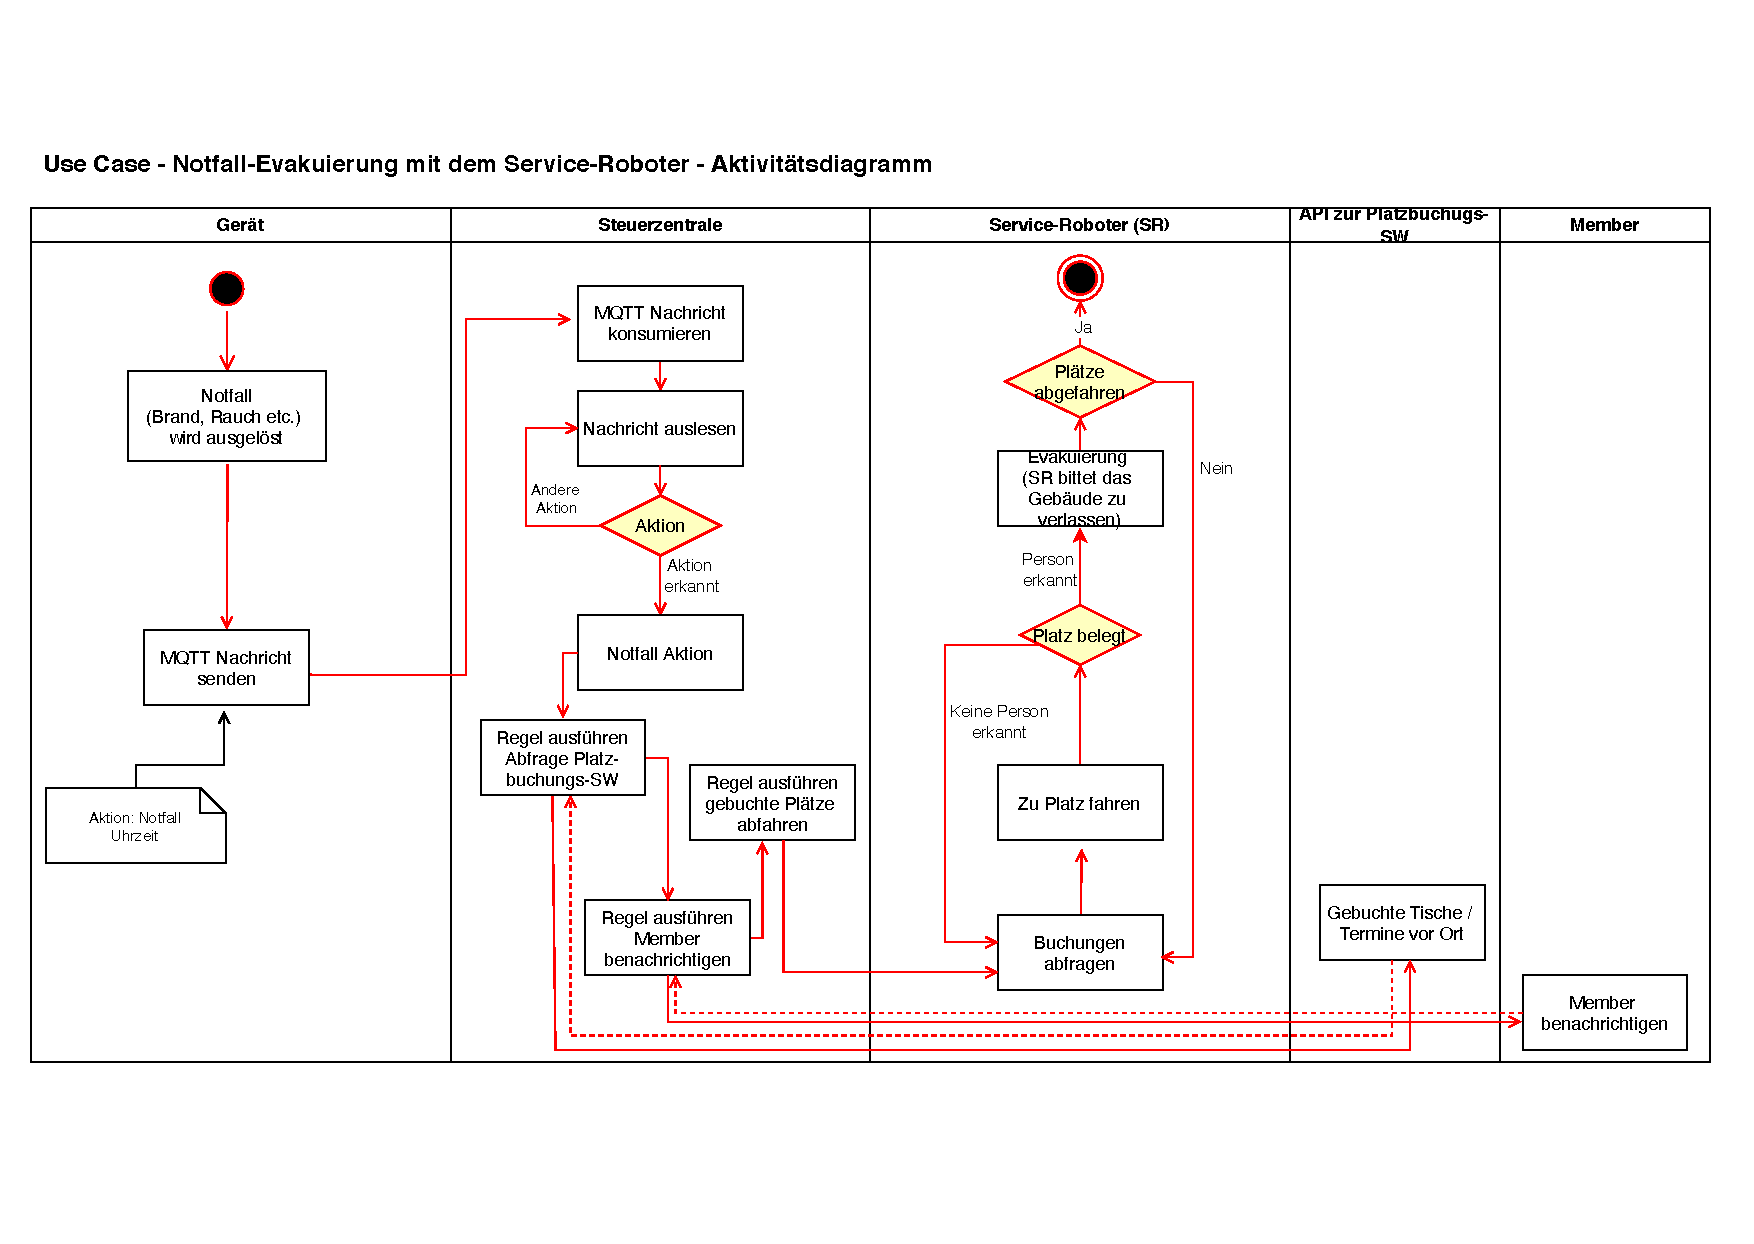
\includepdf[scale=0.75, pages=-, angle=90, fitpaper=true, ]{images/UC2_Aktionsdiagramm_Notfall.pdf}
\end{landscape}
\begin{landscape}
  \AddToShipoutPictureBG*{%
  \AtPageLowerLeft{%
    \raisebox{\dimexpr.5\paperheight-.5\height}{%
      \makebox[.9\paperwidth][r]{%
        \rotatebox{90}
        {\thepage}
      }% \makebox
    }% \raisebox
  }% \AtPageCenter
}% \AddToShipoutPictureBG*
  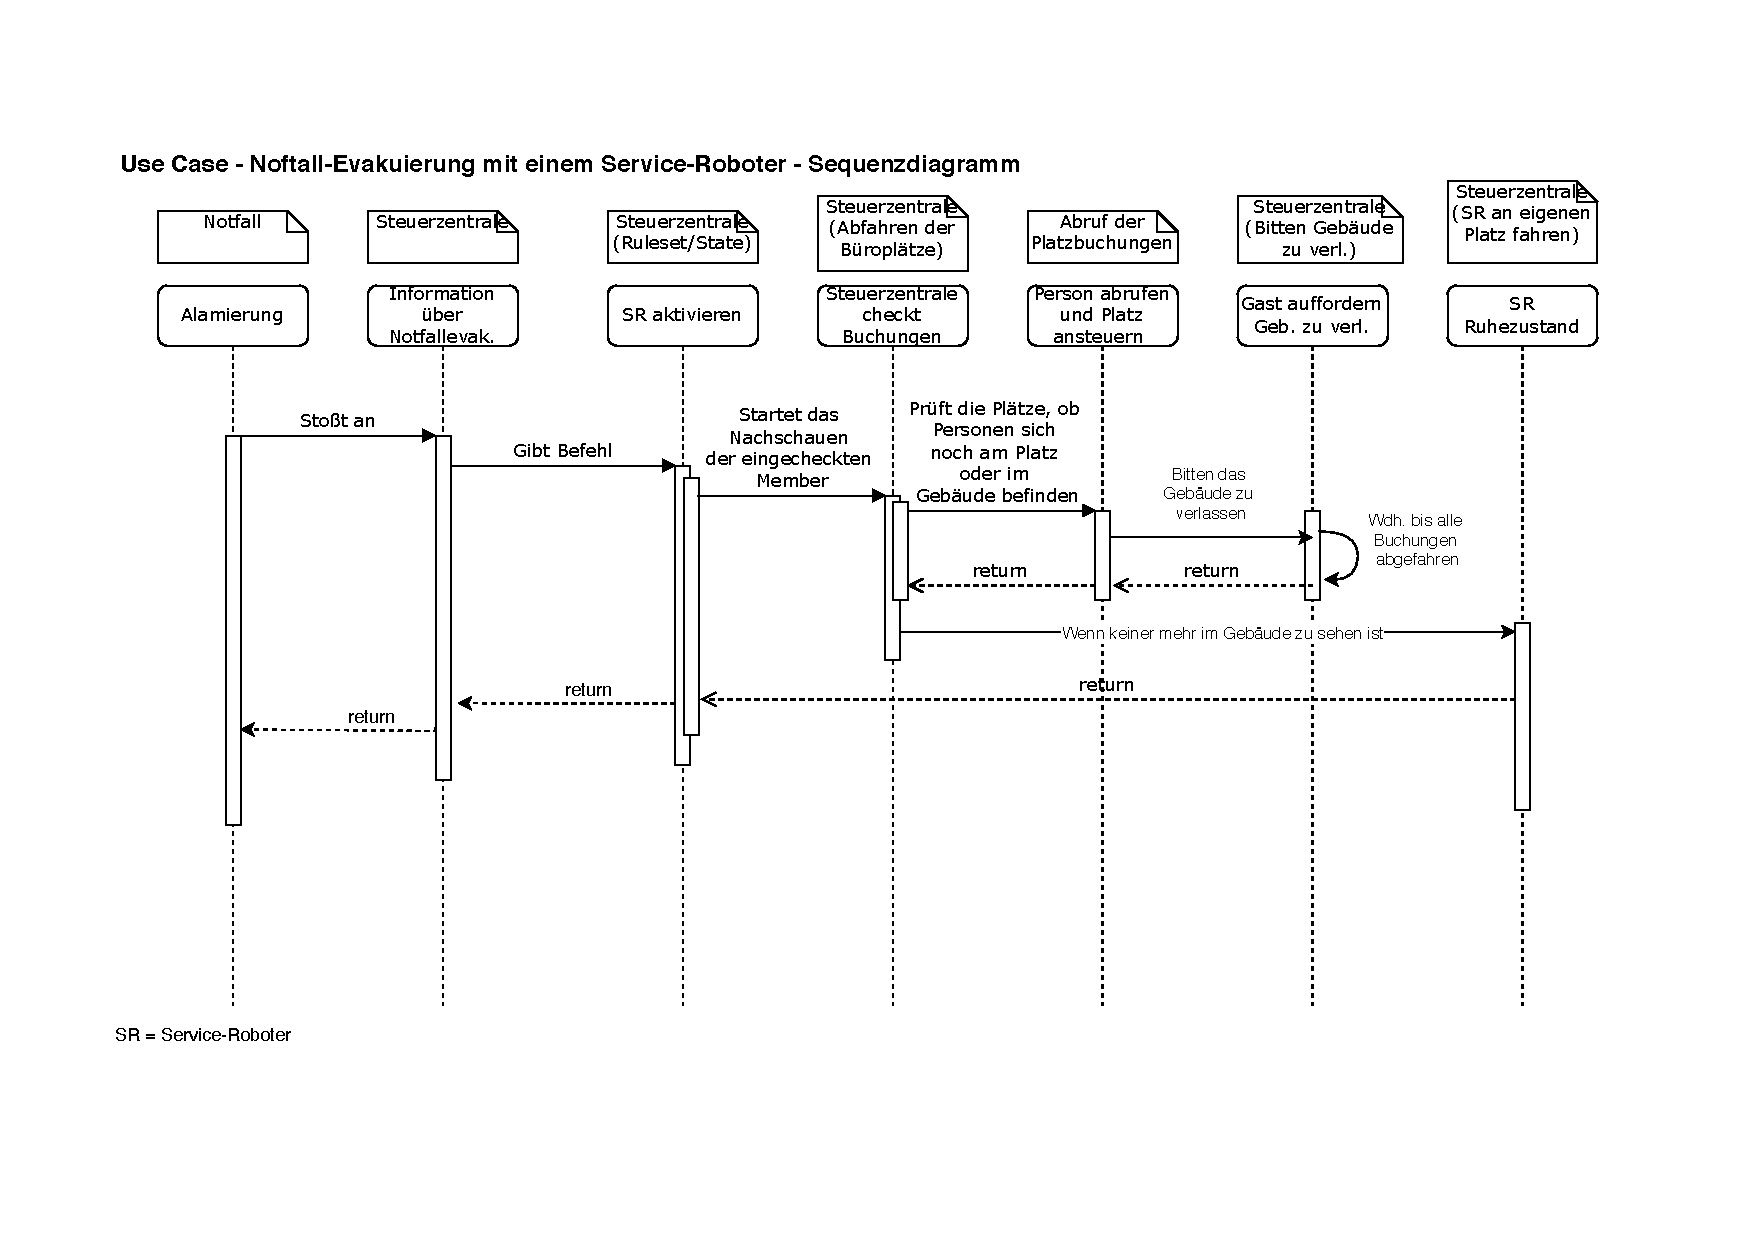
\includepdf[scale=0.75, pages=-, angle=90, fitpaper=true, ]{images/UC2_Sequenzdiagramm_Notfall.pdf}
\end{landscape}
\section{Experteninterview}
\label{sec:experteninterviewReqirements}
    Zur Analyse und Erhebung von Anforderungen, die sich an das System richten, werden Experteninterviews durchgeführt. 
    Dabei wird sich, wie in dem Abschnitt (\ref{subsec:experteninterview}) beschrieben, an dem unstrukturierten Ansatz der 
    Führung eines solchen Interviews orientiert \cite{robson2002real}. Deshalb werden keine konkreten offenen oder 
    geschlossenen Fragen gestellt. Der Aufbau des Interviews wird in weiteren Schritten aufgegriffen. 
    \\
    Die Ergebnisse der Interviews sind nicht repräsentativ, da sie im Rahmen dieser Arbeit mit einigen wenigen Experten durchgeführt wurden. Sie 
    dienen lediglich der Informationsgewinnung und dem Einholen mehrerer Meinungsbilder, um aus allen 
    Ideen, Gedankenanstößen und Ansichten ein Gesamtbild zu erzeugen und daraus mehrere Anforderungen zu gewinnen 
    und abzuleiten. 

\subsection{Ziel des Experteninterviews}
    Ziel des Experteninterviews ist die Informationsgewinnung aus bestimmten Sachverhalten, für die es 
    noch keine repräsentativen Umfragen gibt. Der Experte kann seine Sicht auf den Sachverhalt 
    wiedergeben und neue Blickwinkel eröffnen. Dadurch können Rückschlüsse gezogen und Erfahrungen ausgetauscht werden. Diese sind oft wichtige 
    Informationen zur Erhebung von Anforderungen zu einem bestimmten Sachverhalt. 

\subsection{Aufbau des Experteninterviews}
    Die Experteninterviews wurden im Gesamten als unstrukturierte Interviews durchgeführt. Lediglich die Rahmenbedingungen sowie 
    der Einstieg in das Interview waren vorgegeben und ähneln sich bei jeder interviewten Person. Zu Anfang des Gesprächs wurde 
    der Kontext und die Intension erläutert, damit der Experte die Situation und die Absichten kennenlernt und die 
    eigentliche Herausforderung 
    erkennt. Grundlage dafür war die Erläuterung der Zielsetzung der Arbeit (\ref{sec:zielsetzung}) zur Verdeutlichung der 
    Intension. Mit den identifizierten Anwendungsfällen (\ref{sec:usecases}), die als Basis 
    zur Extraktion von Anforderungen und als potenziell umsetzbare Funktionalitäten gelten, wurden Szenarien veranschaulicht, 
    die dabei halfen, das Anwendungsumfeld zu konkretisieren.  
    Nach der Schilderung des Kontextes und der zugrunde liegenden Ausgangspunkte wurde das Gespräch in Richtung Anforderungen 
    gelenkt. Hierbei lag der Fokus auf dem Sammeln von Ideen, Sichtweisen und Meinungen, die als Grundlage 
    dienten oder gar direkte Anforderungen an das System ergaben. Dabei war der Ausgang des Gesprächs offen. Falls während 
    eines Gespräches der Fokus verloren ging bzw. Exkurse ein zu großes Ausmaß annahmen, wurde wieder auf die 
    vorliegende Sachlage aufmerksam gemacht und der Fokus erneut auf die Anforderungen geworfen. 
    Schwerpunkte bei den Interviews waren zum einen die Anforderungen, welche für eine einfache Handhabung der 
    formalisierten Interaktionen für den Softwareentwickler gelten, und zum anderen die Funktionalitäten, die der 
    Experte dem System gegenüber sieht, um ein Regelwerk für ein intelligentes Büro zu erstellen. 
    Ebenso wurden nicht funktionale Anforderungen, die ein solches System mit sich bringen soll, adressiert. 
    Die zusammengefassten Anforderungen und die daraus abgeleiteten Bedingungen sind dem Abschnitt (\ref{sec:requirementsFinal}) 
    zu entnehmen.
     
\subsection{Zusammenfassung der Experteninterviews}
    In Summe wurden insgesamt fünf Experteninterviews durchgeführt. Jedes Gespräch war individuell und hatte dementsprechend 
    einen anderen Verlauf bzw. ein anderes Ergebnis. Dennoch konnte der inhaltliche Fokus gewahrt und verschiedene 
    Meinungsbilder eingeholt werden. Jeder befragte Experte konnte zu dem anliegenden Sachverhalt seine Meinung äußern und 
    wichtige Informationen und Sichtweisen mitteilen. Die erhobenen Informationen wurden analysiert, aufbereitet und 
    als Anforderungen dokumentiert. Die dabei entstandenen Informationen und Anforderungen werden in 
    folgendem Abschnitt aufgezeigt. 
    
%\pagebreak
\section{Anforderungen}
\label{sec:requirementsFinal}
    In Folge der vorangestellten Literaturrecherche, der Markt- und Zielgruppenanalyse, der entwickelten Anwendungsfälle und 
    der durchgeführten Experteninterviews ergaben sich Anforderungen an das System, 
    die in der Konzeption und der anschließenden prototypischen Implementierung zu berücksichtigen sind. 
    Zur Dokumentation der nicht funktionalen Anforderungen wird sich an dem 
    \textit{Software Produkt Qualitätsmodell} nach der ISO Norm 25010\footnote{Qualitätscharakteristiken nach ISO. \url{https://iso25000.com/index.php/en/iso-25000-standards/iso-25010} Besucht am 24.06.2022.} 
    orientiert. 
    \\
    %\linebreak
    Der folgenden Tabelle (\ref{tab:functionalRequirements}) sind die funktionalen Anforderungen (FA) zu entnehmen: 
    %\pagebreak
    \begin{table}[hbt!]
        \begin{center}
            \begin{tabular}{ | p{0.6cm} | p{9.5cm} | p{1.6cm} | p{3.1cm} | }
                \hline
                    \textbf{} & \textbf{Anforderung (User Story)} & \textbf{Priorität} & \textbf{Quelle} \\
                \hline
                    FA1 & Als Softwareentwickler möchte ich mit einer vorgegebenen Struktur Regeln definieren, die zur Laufzeit ausgeführt werden können. & Essentiell & Zielsetzung der Arbeit \\  %, wenn das zutreffende Ereignis eintrifft.
                \hline
                    FA2 & Als Softwareentwickler möchte ich, dass alle Regeln, die ich definiert habe, zu bestimmtem Auslöser gestartet werden. & Essentiell & Experteninterview \\
                \hline
                    FA3 & Als Softwareentwickler möchte ich einen Zustandsraum erstellen, der individuell implementiert werden kann. & Essentiell & Experteninterview \\ 
                \hline
                    FA4 & Als Softwareentwickler möchte ich Bedingungen definieren und abfragen können, die basierend auf dem Ereignis die dazugehörige Regel ausführen. & Essentiell & Experteninterview \\ 
                \hline
                    FA5 & Als Softwareentwickler möchte ich Komponenten anlegen können, die reelle Gegenstände und dessen Zustände abbilden. & Hoch & Experteninterview \\
                \hline
                    FA6 & Als Softwareentwickler möchte ich das vorgegebene Framework individuell nutzen können, indem ich bei der Definition der Regeln und der Informationsbeschaffung nicht eingeschränkt bin. & Essentiell & Zielsetzung der Arbeit, Experteninterview \\
                \hline
                %    FA7 & Als Softwareentwickler möchte ich Auslöser aktivieren bzw. definieren können, nach denen die Regeln ausgelöst werden. & Essentiell & Experteninterview \\ 
                %\hline
            \end{tabular}
        \end{center}
        \caption{Funktionale Anforderungen (FAs)}
        \label{tab:functionalRequirements}
    \end{table}
    %\\
    %\pagebreak
    %Nach der Aufstellung der funktionalen Anforderungen folgt die der nicht funktionalen Anforderungen (NFA):
   
\begin{table}[hbt!]
    \begin{center}
        \begin{tabular}{ | p{1.0cm} | p{9.7cm} | p{1.6cm} | p{2.6cm} | }
            \hline
                \textbf{} & \textbf{Anforderung} & \textbf{Priorität} & \textbf{Quelle} \\
            \hline
                NFA1 & Benutzerfreundlichkeit (BF): Der Anwender soll nach Implementierung, bzw. Definition einer Regel, diese mit weniger als 3 Schritten in das Regelwerk einfügen können. & Hoch & Experten-interview \\
            \hline
                NFA2 & BF: Mehr als 90\% der Anwender sollten bei erster Verwendung des Frameworks in der Lage sein, Regeln anzulegen und diese dem Regelwerk hinzuzufügen. & Essentiell & Zielsetzung der Arbeit, Experteninterview \\ 
            \hline
                NFA3 & BF: Der Anwender soll die Möglichkeit haben, zu dem Zeitpunkt der Verwendung des Frameworks alle verfügbaren Funktionen nutzen und anwenden zu können. & Mittel & Experten-interview \\ 
            \hline
                NFA4 & BF: Der Anwender braucht sich zu keinem Zeitpunkt um das Management, bzw. um den Ablauf und Durchführung von Regeln kümmern. Er muss nur sicherstellen, dass die Regeln valide sind und dem Kontext passende Bedingungen und Regelausführungen festlegt. & Essentiell & Experten-interview \\ 
            \hline
                NFA6 & Zuverlässigkeit (Z): Zeitlich gebundene Regeln sollen immer zu der vorgegebenen Uhrzeit ausgelöst werden. & Hoch & Experten-interview \\
            \hline
                NFA5 & Z: Als Anwender möchte ich, dass zu 100\% die Regel ausgeführt wird, die der Auslöser ansteuert. (Bei sequenzieller Ausführung soll immer die Regel gestartet werden, die durch den Auslöser ausgelöst wurde.) & Essentiell & Experten-interview \\
            \hline
                NFA7 & Performanz (P): Ausgelöste Regeln, die beide voneinander unabhängige Ressourcen, bzw. einen Wert im Zustandsraum belegen, sollen parallel ausgeführt werden. & Hoch & Anwendungsfall, Experten-interview \\ 
            \hline
                NFA8 & P: Regeln, die über Kommunikationsprotokolle ausgelöst werden, sollen unter einer Sekunde starten. Die Zeit der Durchführung ist abhängig von der Regel selbst. & Mittel & Anwendungsfall, Experten-interview \\ 
            \hline
                NFA9 & Verfügbarkeit (V): Die Steuerzentrale muss eine Verfügbarkeit von 99,9\% vorweisen. (Zum aktuellen Zeitpunk ist diese Anforderung zu vernachlässigen.) & Niedrig & Experten-interview \\ 
            \hline
                NFA10 & V: Die Steuerzentrale muss während der Arbeitszeiten zwischen 7-18 Uhr ohne Ausfälle verfügbar sein. (Zum aktuellen Zeitpunk ist diese Anforderung zu vernachlässigen.) & Niedrig & Experten-interview \\ 
            \hline
                NFA11 & Fehlertoleranz: Syntaktisch oder inhaltlich fehlerhafte Regeln sollen nicht zum Absturz der Steuerzentrale führen. & Mittel & Experten-interview \\ 
            \hline  
                NFA12 & Kontrollierbarkeit, Beobachtbarkeit: Prozesse und Zustände der Steuerzentrale müssen eingesehen werden können, bspw. durch Monitoring oder über Oberflächen. (Zum aktuellen Zeitpunkt zu vernachlässigen.) & Niedrig & Experten-interview \\
            \hline
        \end{tabular}
    \end{center}
    \caption{Nicht funktionale Anforderungen (NFAs)}
    \label{tab:notfunctionalRequirements}
\end{table}
\subsubsection*{}
Eine Auswahl an zusätzlichen Anforderungen, die ergänzend zu den bereits Bestehenden aus der Zielgruppenanalyse und den Anwendungsfällen entstanden sind und sowohl die funktionalen 
(\ref{tab:functionalRequirements}) als auch die nicht funktionalen Anforderungen (\ref{tab:notfunctionalRequirements}) erweitern, ist der folgenden 
Tabelle zu entnehmen. Diese sind als zusätzliche Anforderungen (ZAF) gekennzeichnet: 
\begin{table}[hbt!]
    \begin{center}
        \begin{tabular}{ | p{1.0cm} | p{9.2cm} | p{1.6cm} | p{3.1cm} | }
            \hline
                \textbf{} & \textbf{Anforderung} & \textbf{Priorität} & \textbf{Quelle} \\
            \hline
                ZAF1 & Zur Entwicklung des Frameworks soll Java als Programmiersprache verwendet werden. & Hoch & Experteninterview, Zielgruppenanalyse \\ 
            \hline
                ZAF2 & Die Abbildung von Komponenten soll über einen Zustandsraum dargestellt werden. & Niedrig & Anwendungsfall, Experteninterview \\ 
            \hline
                ZAF3 & Zur parallelen Ausführung von Regeln soll ein Thread Pool eingesetzt werden, der die Regeln jeweils als eigenen Thread laufen lässt. & Hoch & Anwendungsfall, Experteninterview \\ 
            \hline
                ZAF4 & Regeln sollen über zeitbasierte oder MQTT basierte Auslöser gestartet werden, nachdem die dafür vorgesehene Bedingung zutrifft. (Im Rahmen der Anwendungsfälle wird MQTT als Kommunikationsprotokoll und Auslöser gewählt.) & Hoch & Anwendungsfall \\
            \hline
                ZAF5 & Regeln und damit einhergehende Aktionen dürfen erst nach aktivieren eines bestimmten Auslösers (Triggers) ausgeführt werden. & Essentiell & Experteninterview \\
            \hline
                ZAF6 & Der Zustandsraum muss zur Laufzeit zur Verfügung stehen. & Hoch & Experteninterview \\ 
            \hline
                ZAF7 & Die Kommunikation erfolgt überwiegend durch MQTT. & Hoch & Anwendungsfall \\ 
            \hline
                ZAF8 & Sicherheit: Die Kommunikation soll über einen MQTT Broker im eigenen Netzwerk erfolgen. Das System soll nach außen nicht erreichbar sein. & Hoch & Experteninterview \\
            \hline
                ZAF9 & Bereitstellung eines \ac{SPC} (Implementierung, Anpassung und Erweiterung der Regel und der Logik). & Hoch & Zielgruppenanalyse, Experteninterview \\ 
            \hline
            %    ZAF10 & Die Zustände der Komponenten sollen persistiert werden, damit bei einem Systemausfall die letzten Transaktionen und Änderungen nachvollzogen werden können. (Ist zur Konzeption zu berücksichtigen, Priorität aus dem Proof of Concept (PoC) jedoch gering.) & Niedrig & Experteninterview \\ 
            %\hline 
        \end{tabular}
    \end{center}
    \caption{Zusätzliche Anforderungen}
    \label{tab:furtherRequirements}
\end{table} 
\\
Alle relevanten Anforderungen, die mithilfe den genannten und durchgeführten Erhebungsmethoden eruiert wurden, fließen in die Konzeption 
des Frameworks mit ein. Diese bilden die Grundlage des Konzeptes. 

\chapter{Konzeption}
\label{chap:konzept}
    In diesem Kapitel wird das erarbeitete Konzept dieser Arbeit dargelegt. Basierend auf den 
    Anforderungen, die aus den Anwendungsfällen, Experteninterviews und der Zielgruppenanalyse 
    erhoben wurden, werden die daraus generierten Überlegungen und Entscheidungen transparent 
    dargestellt. Durch die bereits erfolgten Schritte der Anforderungsanalyse (\ref{chap:anforderungsanalyse})
    sind erste Aufgaben der Konzeption abgeschlossen. 
    \\
    Zu Anfang des Kapitels wird das allgemeine Ziel eines Konzeptes erläutert. Anschließend 
    wird auf das Anwendungsumfeld des Systems, engl. Framework, (\ref{sec:anwendungsumfeld}) eingegangen. 
    % die abzudeckenden Funktionalitäten (\ref{sec:konzeptfunktionalitaet}), die 
    %aus den Anforderungen ermittelt wurden, eingegangen. 
    Darauf folgend wird anhand den 
    zugrundeliegenden Informationen das Architekturkonzept (\ref{sec:architekturkonzept}), sowie das 
    Softwarekonzept (\ref{sec:softwarekonzept}) erläutert. Des Weiteren werden die Hintergründe der 
    Wahl des Frameworks (\ref{sec:frameworkauswahl}) aufgezeigt. %Abschließend wird das konzipierte 
    % und prototypische Datenmodell \ref{sec:...} dargelegt. 

\section{Ziel der Konzeption}
\label{sec:konzeptziele}
    Das Ziel einer Konzeption ist die Veranschaulichung von abstrakten Ideen, geistiger Entwürfe und Leitideen. 
    Hierbei werden aus den zugrundeliegenden Problemstellungen, Szenarien und Anforderungen Entwürfe und 
    Lösungsmöglichkeiten erarbeitet und identifiziert. Diese helfen bei der Aufstellung von notwendigen Schritten 
    und dienen als Grundlage zur Untermauerung und Darlegung von Entscheidungen. Somit wird Dritten der Kontext, die 
    Domäne und das zu lösende Problem, bzw. die Lösung dargestellt. 
    \\
    \linebreak
    Im Rahmen dieser Arbeit ist das Ziel des Konzeptes die Veranschaulichung der Entscheidungsfindung zur Lösung des vorliegenden 
    Sachverhaltes. Das Konzept 
    erarbeitet eine Lösung zur Implementierung einer Anwendung zur Koordination von Regeln und Prozessen innerhalb eines 
    Firmenbüros. Hierbei wird der allgemeine Aufbau der Architektur skizziert und demonstriert, wie eine solche Lösung aussehen kann. 
    Unter Berücksichtigung der Forschungsfrage (siehe Abschnitt \ref{sec:forschungsfragen}) wird eine Möglichkeit offengelegt, mit der 
    ein Softwareentwickler neue Regeln entwickeln und dem System hinzufügen kann, ohne ein weiteres zu erlernendes Framework zu verwenden. 
    Dabei sollen die notwendigen Schritte und Interaktionen formalisiert und für den Entwickler vereinfacht werden. Mit der 
    Definition der Zielsetzung der Arbeit (siehe Abschnitt\ref{sec:zielsetzung}) wird die Abgrenzung deutlich. In folgender 
    Darlegung des Konzeptes wird nochmals konkreter auf den Kontext als auch auf die Intension eingegangen. 
    % Das Ziel des Konzeptes ist es, dem Entwickler den Aufwand zur Erweiterung des Systems zu minimieren durch weitere 
    % Regeln und Abdeckung von Anwendungsfällen (Use Cases) und eine Struktur vorgeben. (ToDo's, Flexibilität in der 
    % Umsetzung (nicht wie Home Assistant und openHAB eher eingeschränkt)) 

%\section{Abzudeckende Funktionalitäten}
%\label{sec:konzeptfunktionalitaet}
    % Was soll der Entwickler machen können? 
    % Welche Grundlagen braucht er, um eine Regel implementieren zu können?
    % Welche Funktionen müssen gegeben sein, um die Struktur vorzugeben? 
    % Reicht ein Hinweis weöche Stellen angepackt werden müssen, um eine Regel hinzuzufügen? 
    
    %%%%%%%%%%%%%%%%%%%%%%%%%%%%%%%%%%%%%%%%%%%%%%%%%%%%%%%%%%%%%

    % ZIEL DES KONZEPTES: Ein Framework für Entwickler bereitzustellen, welches die Mächtigkeit für den Entwickler offen lässt, nicht einschränkt 
    % und dennoch Konfiguration und Ausführung umsetzt. Der Entwickler muss lediglich den Zustandsraum, die MQTT-Topics und die Regeln definieren.
    % Der Entwickler bekommt ein Framework in die Hand, welches die Umsetzung von Prozessen in einem smarten Büro ermöglicht. Das Framework kümmert sich um die 
    % Organisation und die Ausführung der Regeln. Die Richtigkeit der Regeln und des Zustandsraumes muss der Entwickler sicherstellen. 
    % Die Kommunikation über MQTT ist nur eine Möglichkeit. Des Setup wird wegabstrahiert 

    %%%%%%%%%%%%%%%%%%%%%%%%%%%%%%%%%%%%%%%%%%%%%%%%%%%%%%%%%%%%%

\section{Anwendungsumfeld}
\label{sec:anwendungsumfeld}
    Grundsätzlich ist der Einsatzort des Frameworks variabel, da die eigentliche Implementierung und Nutzung der Regeln und Prozesse stark 
    abhängig von den Anwendern ist. Dadurch kann sowohl in privatem \acl{SH} Umfeld als auch in Büroräumen eine solche Instanz mittels dem 
    Framework erstellt werden. Basierend auf den vorangestellten Tätigkeiten, darunter die Anforderungsanalyse und die Eingrenzung auf den 
    Einsatz im Smart Office, liegt der Schwerpunkt auf dem Einsatz in einem smarten Büro. 

\section{Architekturkonzept}
\label{sec:architekturkonzept}
    % Es wird alles abgebildet über einen Zustandsraum, der sich aus den Dingen (Gegenständen) und Zuständen der Anwendung ergibt.
    % Der Zustandsraum wird verändert, wenn eine Aktion durchgeführt wird, bzw. durch eine Trigger angestoßen. 
    % Bzw. speichert den aktuellen Zustand des Gegenstandes 
    % (lightBulb = true/false, personOnDoor = null/Mikka, booking = stringBooking, temiAktive = true/false, 
    % temiPosition = stringKoordinates)
    % Zustandsraum muss von dem Entwickler definiert werden. 
    % MQTT Broker über Home Assistant, bzw. losgelöster Broker
    % Anbindung von APIs auch Entwickler-Sache. Kann ich das vereinfachen, sodass die Integration einfacher wird?

    \subsection{Überlegungen, Anstöße und Herausforderungen}
    % Regeln über Thread abbilden? Ja, Nein? - Nein, wieso? Da Durch die MQTT Message mehrere Regeln ausgeführt 
    %werden können. -> Lediglich den Zustand der Komponenten locken.
    % KEIN THREAD (wird schon abgebildet durch die Services und die Auslöser durch MQTT), Falls eine Komponente 
    %  doppelt beansprucht wird, ist der Zustand der Komponenten zu locken und ein 
    % Thread.sleep einzurichten. Abfrage, ob der Wert, bzw. die Komponente wieder freigegeben wurde. 

    % Zustandsraum -> Abbildung aller notwendigen Komponenten 
    % Bei Bearbeitung einer Regeln die Komponenten Locken, sodass nur die einzelne Komponenten (deren Zustand) gelockt ist 
    % und nicht der ganze Zustandsraum, somit können mehrere Komponenten und Aktionen ausführen zu können. 

    %Was brauche ich für Funktionen und Werte in einer Regel?

    % Ein Zustandsraum (Objekt) für alles oder ein Globales, welches die die Komponenten enthält? - Begründung für die Auswahl.
    
    \subsection{Schnittstellen}
        % Kommunikation mit API's je nach Use Case und Gebrauch zur Datenabfrage
    
    \subsection{Datenbanken}
        % Datenbanken je nach Use Case und Gebrauch zur Datenabfrage

\section{Softwarekonzept}
\label{sec:softwarekonzept}

\section{Auswahl des Frameworks}
\label{sec:frameworkauswahl}
    Im Bereich der Java-Entwicklung gibt es mittlerweile viele Möglichkeiten, um Applikationen, Anwendungen und Frameworks 
    zu entwickeln, die unterschiedliche Präferenzen und Einsatzmöglichkeiten bieten. Dadurch sind, auf den Einsatzbereich bezogen, 
    Vor- und Nachteile im Vergleich ähnlicher Systeme nicht auszuschließen. Eine kleine Auswahl an Systemen wurde getestet und auf deren 
    Brauchbarkeit analysiert und evaluiert. Für diese Evaluation wurden Kriterien ausgearbeitet, mit der die Auswahl des Frameworks 
    eingeschränkt und nach Möglichkeit das passende ergeben soll. Diese sind nach ihrer Relevanz aufgelistet: 
    \begin{enumerate}
        \item Freiheiten bei der Nutzung (Anwendung und Gewährleistung von Entwurfsmustern).
        \item Nutzung und Bereitstellung von Bibliotheken (Libraries).
        \item Bereitstellung einer Plattform (Full Stack).
        \item Aktive Community und stetige Weiterentwicklung des Systems.
        \item Nutzung des Frameworks in bereits bestehenden Projekten im Bereich Smart Home.
        \item Open Source-Projekt, um Flexibilität und weitestgehende Unabhängigkeit zu gewährleisten.
        \item Ausschluss von Frameworks, die ausschließlich für die Web-Entwicklung gedacht sind.
    \end{enumerate}  
    Aufgrund der Vielzahl an Frameworks war es im Rahmen dieser Arbeit nicht möglich, alle vorhandenen und in Betracht 
    gezogenen Systeme detailliert aufzuführen. Lediglich die engere Auswahl wird aufgegriffen. 
    Nach ausführlicher Recherche und unter Berücksichtigung von Frameworks, wie bspw. Grails, Quarkus, Blade, und Play, wurden 
    schließlich genau zwei Systeme gegenübergestellt, die die vorangestellten Kriterien in Gänze erfüllen. Viele in Betracht gezogenen Frameworks 
    finden überwiegend in der Web-Entwicklung Anwendung, bzw. basieren auf dem Spring Framework. Durch diese Erkenntnis wurden 
    viele Systeme nicht weiter berücksichtigt und betrachtet. Die beiden Kernsysteme, die ihren Einsatz und ihre Möglichkeiten rechtfertigen
    werden in den folgenden Abschnitten kurz erläutert.

    \subsection{OSGi}
    \label{subsec:osgiFramework}
        Das \ac{OSGI} Framework, welches in der openHAB Software eingesetzt wird, der \acs{OSGI}\footnote{Ursprung der OSGi Plattform. \url{https://www.osgi.org/about/} Abgerufen am 19.06.2022} 
        Alliance klassifiziert eine dynamische Softwareplattform, mit der die Modularisierung und Verwaltung von Applikationen und 
        den dazugehörigen Diensten mittels Komponentenmodell realisiert werden kann \cite{funke2009}. Bekannte Produkte, die auf der 
        \acs{OSGI} Plattform laufen, sind neben openHAB unter anderem die Entwicklungsumgebung Eclipse der Eclipse Foundation, Produkte 
        und Softwarelösungen von IBM, Oracle, Adobe und weitere. 
        \\
        Nennenswerte Eigenschaften und Vorteile der Software sind die Modularisierung und Versionierung, das zur Laufzeit organisierte 
        Abhängigkeitsmanagement, das Fernmanagement des laufenden Systems über sogenannte Management Agents und die Nutzung des 
        Serviceorientiert Programmiermodell. An dieser Stelle wird das Framework nicht technisch vertieft. Die Funktionsweise und die technisch 
        fundierte Erläuterung kann dem Buch \cite{osgibuch}, sowie der Dokumentation \cite{osgipraesentation} eines ausgearbeiteten Workshops entnommen werden. 
        Nachteile der Plattform ist zum einen der weniger breite Einsatz des Frameworks und die kleine Community. 
        Ebenso findet eine Weiterentwicklung der Plattform nur mäßig statt. 

    \subsection{Spring Boot}
    \label{subsec:springBootFramework}




\begin{landscape}
  \AddToShipoutPictureBG*{%
  \AtPageLowerLeft{%
    \raisebox{\dimexpr.5\paperheight-.5\height}{%
      \makebox[.9\paperwidth][r]{%
        \rotatebox{90}
        {\thepage}
      }% \makebox
    }% \raisebox
  }% \AtPageCenter
}% \AddToShipoutPictureBG*
  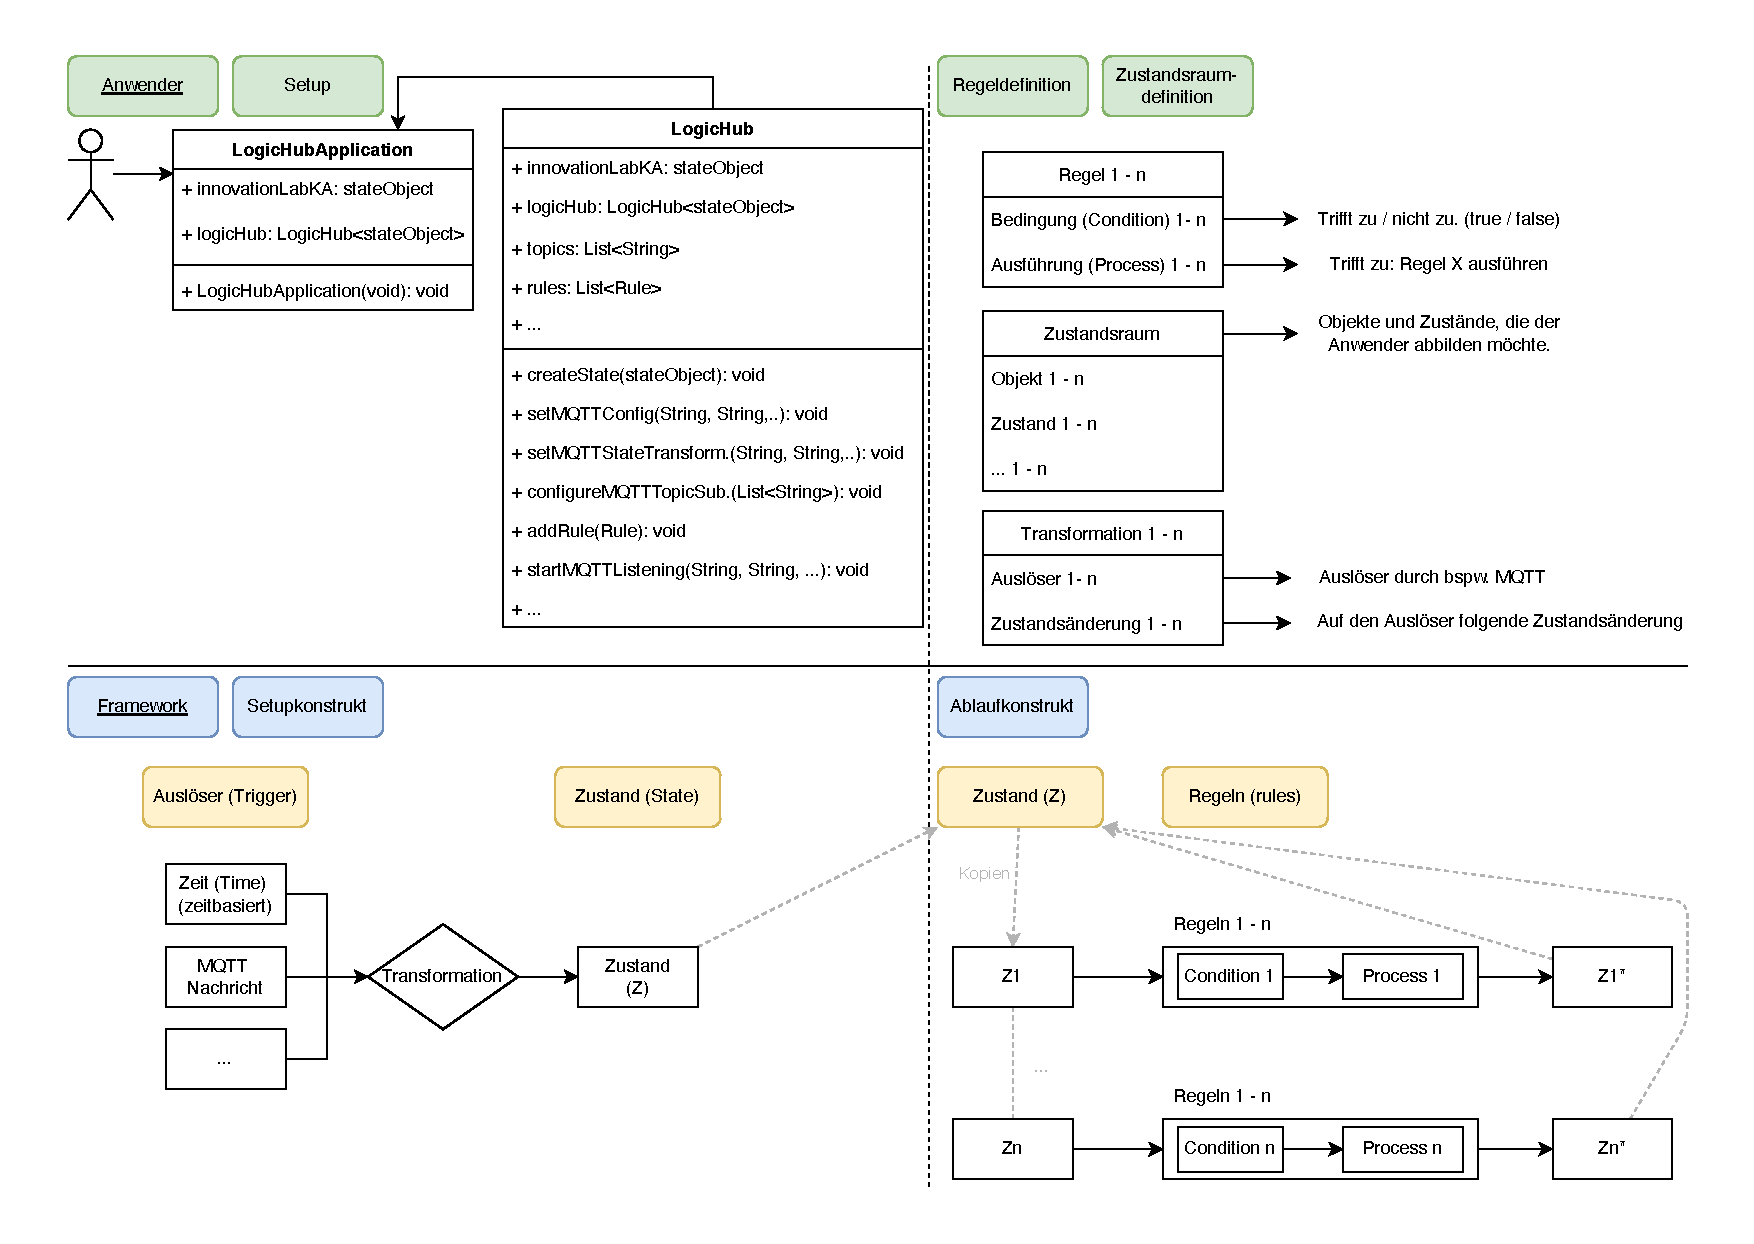
\includepdf[scale=0.75, pages=-, angle=90, fitpaper=true, ]{images/konzept_MA.pdf}
\end{landscape}
\section{Architekturkonzept}
\label{sec:architekturkonzept}
    Das Framework stellt die Kern-Funktionalität zur Steuerung von Prozessen innerhalb eines Büroraumes dar. Diese kann als 
    Logikschicht in ein gesamtheitliches System integriert werden. Potentielle Erweiterungen und Integrationen werden im Ausblick 
    (\ref{chap:ausblick}) nochmals aufgegriffen. Das Architekturkonzept umfasst ausschließlich die grundlegende Funktion des 
    Frameworks der Steuerzentrale. 
    % Es wird alles abgebildet über einen Zustandsraum, der sich aus den Dingen (Gegenständen) und Zuständen der Anwendung ergibt.
    % Der Zustandsraum wird verändert, wenn eine Aktion durchgeführt wird, bzw. durch eine Trigger angestoßen. 
    % Bzw. speichert den aktuellen Zustand des Gegenstandes 
    % (lightBulb = true/false, personOnDoor = null/Mikka, booking = stringBooking, temiAktive = true/false, 
    % temiPosition = stringKoordinates)
    % Zustandsraum muss von dem Entwickler definiert werden. 
    % MQTT Broker über Home Assistant, bzw. losgelöster Broker
    % Anbindung von APIs auch Entwickler-Sache. Kann ich das vereinfachen, sodass die Integration einfacher wird?

    \subsection{Überlegungen, Anstöße und Herausforderungen}
    % Regeln über Thread abbilden? Ja, Nein? - Nein, wieso? Da Durch die MQTT Message mehrere Regeln ausgeführt 
    %werden können. -> Lediglich den Zustand der Komponenten locken.
    % KEIN THREAD (wird schon abgebildet durch die Services und die Auslöser durch MQTT), Falls eine Komponente 
    %  doppelt beansprucht wird, ist der Zustand der Komponenten zu locken und ein 
    % Thread.sleep einzurichten. Abfrage, ob der Wert, bzw. die Komponente wieder freigegeben wurde. 

    % Zustandsraum -> Abbildung aller notwendigen Komponenten 
    % Bei Bearbeitung einer Regeln die Komponenten Locken, sodass nur die einzelne Komponenten (deren Zustand) gelockt ist 
    % und nicht der ganze Zustandsraum, somit können mehrere Komponenten und Aktionen ausführen zu können. 

    %Was brauche ich für Funktionen und Werte in einer Regel?

    % Ein Zustandsraum (Objekt) für alles oder ein Globales, welches die die Komponenten enthält? - Begründung für die Auswahl.
    
    \subsection{Schnittstellen}
        % Kommunikation mit API's je nach Use Case und Gebrauch zur Datenabfrage
    
    \subsection{Datenbanken}
        % Datenbanken je nach Use Case und Gebrauch zur Datenabfrage

\subsection{Softwarekonzept}
\label{subsec:softwarekonzept}




\chapter{Umsetzung}
\label{chap:umsetzung}
    Im Rahmen einer prototypischen Implementierung wurde das im Kapitel Konzeption (\ref{chap:konzept}) geplante Systems 
    umgesetzt. Gegenstand dieses Kapitels wird es sein, Aspekte der Umsetzung widerzuspiegeln und konkret die Umsetzung eines  
    Anwendungsfalls darzulegen. Zusätzlich wird die Auswahl des dafür genutzten Frameworks aufgegriffen. 

\section{Auswahl des Frameworks}
\label{sec:frameworkauswahl}
    Im Bereich der Java-Entwicklung gibt es mittlerweile viele Möglichkeiten, um Applikationen, Anwendungen und Frameworks 
    zu entwickeln, die unterschiedliche Präferenzen und Einsatzmöglichkeiten bieten. Dadurch sind, auf den Einsatzbereich bezogen, 
    Vor- und Nachteile im Vergleich ähnlicher Systeme nicht auszuschließen. Eine kleine Auswahl an Systemen wurde getestet und auf deren 
    Brauchbarkeit analysiert und evaluiert. Für diese Evaluation wurden Kriterien ausgearbeitet, mit der die Auswahl des Frameworks 
    eingeschränkt und nach Möglichkeit das passende ergeben soll. Die Kriterien sind nach ihrer Relevanz aufgelistet: 
    \begin{enumerate}
        \item Freiheiten bei der Nutzung (Anwendung und Gewährleistung von Entwurfsmustern).
        \item Nutzung und Bereitstellung von Bibliotheken (Libraries).
        \item Bereitstellung einer Plattform (Full Stack).
        \item Aktive Community und stetige Weiterentwicklung des Systems.
        \item Nutzung des Frameworks in bereits bestehenden Projekten im Bereich Smart Home.
        \item Open Source-Projekt, um Flexibilität und weitestgehende Unabhängigkeit zu gewährleisten.
        \item Ausschluss von Frameworks, die ausschließlich für die Web-Entwicklung gedacht sind.
    \end{enumerate}  
    Aufgrund der Vielzahl an Frameworks war es im Rahmen dieser Arbeit nicht möglich, alle vorhandenen und in Betracht 
    gezogenen Systeme detailliert aufzuführen. Lediglich die engere Auswahl wird aufgegriffen. 
    Nach ausführlicher Recherche und unter Berücksichtigung von Frameworks, wie bspw. Grails, Quarkus, Blade, und Play, wurden 
    schließlich genau zwei Systeme genauer betrachtet, die die vorangestellten Kriterien in Gänze erfüllen. Viele in Betracht gezogenen Frameworks 
    finden überwiegend in der Web-Entwicklung Anwendung, bzw. basieren auf dem Spring Framework. Durch diese Erkenntnis wurden 
    viele Systeme nicht weiter berücksichtigt. Die beiden Kernsysteme, die ihren Einsatz und ihre Möglichkeiten rechtfertigen
    werden in den folgenden Abschnitten kurz erläutert.

    \subsection{OSGi}
    \label{subsec:osgiFramework}
        Das \ac{OSGI} Framework der \acs{OSGI}\footnote{Ursprung der OSGi Plattform. \url{https://www.osgi.org/about/} Abgerufen am 19.06.2022} 
        Alliance, welches in der openHAB Software eingesetzt wird, klassifiziert eine dynamische Softwareplattform, mit der die Modularisierung 
        und Verwaltung von Applikationen und den dazugehörigen Diensten mittels Komponentenmodell realisiert werden kann \cite{funke2009}. Bekannte 
        Produkte, die auf der \acs{OSGI} Plattform laufen, sind neben openHAB unter anderem die Entwicklungsumgebung Eclipse der Eclipse 
        Foundation, Produkte und Softwarelösungen von IBM, Oracle, Adobe und weitere. 
        \\
        Nennenswerte Eigenschaften und Vorteile der Software sind die Modularisierung und Versionierung, das zur Laufzeit organisierte 
        Abhängigkeitsmanagement, das Fernmanagement des laufenden Systems über sogenannte Management Agents und die Nutzung des 
        Serviceorientierten Programmiermodells, \ac{SOA}\footnote{Erläuterung des SOA Modells. \url{https://www.ibm.com/cloud/learn/soa} Abgerufen am 20.06.2022}. 
        An dieser Stelle wird das Framework nicht technisch vertieft. Die Funktionsweise und die technisch 
        fundierte Erläuterung kann dem Buch \cite{osgibuch}, sowie der Dokumentation \cite{osgipraesentation} eines ausgearbeiteten Workshops entnommen werden. 
        Nachteile der Plattform sind zum einen der weniger breite Einsatz des Frameworks und zum anderen die kleine Community. 
        Ebenso findet eine Weiterentwicklung der Plattform nur mäßig statt. Dies hat zur Folge, dass die Erweiterung, bzw. die Entwicklung des darauf 
        aufbauenden Systems träge vonstattengeht. 
        %Wieso Spring Boot und nicht OSGi?
        %Wieso Java und nicht Python oder andere?

    \subsection{Spring}
    \label{subsec:springBootFramework}
    Spring\footnote{Open-Source-Framework Spring. \url{https://spring.io} Abgerufen am 02.07.2022} ist ein Open-Source-Framework, welches auf der Java-Plattform aufbaut. 
    Das Ziel von Spring selbst ist die Vereinfachung und Förderung von Programmierpraktiken in der Java- und Java EE Entwicklung. Mit einem breiten Spektrum an 
    Funktionalitäten bietet das Framework eine ganzheitliche Lösung zur Entwicklung von Applikationen, Anwendungen und Frameworks. Im Vordergrund dabei steht immer die 
    Entkopplung von Applikationskomponenten. Das Spring Framework wurde im März 2004 offiziell Freigegeben und wird seitdem stetig weiterentwickelt. 
    Initiator des Frameworks ist der Author und Softwareentwickler Rod Johnson. Das Framework, welches in dem Buch des Experten Rod Johnson erläutert wird, basiert auf 
    den folgenden Prinzipien \cite{johnson2004expert}: 
    \\
    \linebreak
    Dependency Injection ist ein sehr bekanntes Entwurfsmuster. Dabei werden die Abhängigkeiten eines Objektes zur Laufzeit reglementiert. Unter 
    Verwendung des Frameworks werden den Objekten die benötigten Objekte und Ressourcen zugewiesen. Dadurch müssen diese nicht selbst gesucht werden. 
    \\
    \linebreak
    Ein weiterer Punkt ist die aspektorientierte Programmierung, durch die der Entwickler technische Aspekte voneinander isolieren und den eigentlichen Programmcode 
    von Transaktionen oder anderen Faktoren freizuhalten. 
    \\
    \linebreak
    Das dritte Prinzip ist das Bereitstellen von Vorlagen zur Vereinfachung der Nutzung von Schnittstellen, sog. \acs{API}s. Dadurch wird ein POJO-basiertes Modell 
    möglich. Unter POJO, \textit{Plain Old Java Object}, ist ein ganz normales Objekt in Java zu verstehen. 
    \\
    \linebreak
    Zusammenfassend sind beide Frameworks dazu geeignet, um das Konzept der Steuerzentrale unterstützend zu realisieren. 
    Ein direkter Vergleich zwischen den Frameworks kann nicht gezogen werden, da die Funktionalitäten, bzw. die aus der Nutzung 
    profitablen Eigenschaften nicht vergleichbar sind. Während sich Spring auf die Unterstützung zur Erstellung von Applikationen konzentriert, 
    legt \acs{OSGI} den Mehrwert auf die Modularisierung durch Kontainerisierung. Durchaus ist eine Kombination aus beiden 
    Frameworks möglich, um Vorteile beider zu vereinen. Fundamental bietet Spring jedoch weitaus mehr Möglichkeiten und Unterstützungen 
    zur Entwicklung von Applikationen und Frameworks, weshalb es im Rahmen dieser Arbeit eingesetzt wird. Mit Spring Boot, welches auf Spring 
    aufbaut können auch \acl{MVC} Web-Architekturen und \acs{REST} \acs{API}s implementiert werden. So kann mit dieser Entscheidung 
    ein Vollumfängliches System erstellt werden. Unter zusätzlicher Verwendung von \acs{OSGI} wäre eine weiter Modularisierung und Kontainerisierung möglich. Dies 
    ist auch durch Spring mit Hilfe von Microservices in einer anderen Form realisierbar. 
    \\
    An der Stelle wird im Rahmen dieser Arbeit das Thema von Microservices und Kontainerisierung nicht weiter konkretisiert.
    \\
    \linebreak
    Die Entscheidung viel auf Spring, da dieses ein modernes und etabliertes Framework darstellt und die 
    Community erheblich größer ist, als die des \acs{OSGI} Frameworks. Hinzukommt, die Schaffung eines alternativen Ansatzes zu openHAB, da dieses System bereits 
    auf \acs{OSGI} aufbaut. 
    Dennoch unterscheidet sich die Steuerzentrale in den Funktionalitäten und Angeboten immens im Vergleich zu openHAB. Das System bietet weitaus mehr 
    Funktionalitäten, Erweiterungen und Ausprägungen. Lediglich kann zum Vergleich die Definition von Regeln herangezogen werden. 

\section{Implementierung}
\label{sec:implementation}

\subsection{Generische Programmierung} % Typisierung
% Erledigt! -> WICHTIG!!!: Verwendung der Typisierung, um dem Anwender die Möglichkeit der offenen Gestaltung des Zustandobjektes zu gewährleisten.
Eine entscheidende konzeptionelle Überlegung in Richtung des Zustandsraumes wird vorab erläutert, damit in 
folgenden Darstellungen klar zwischen der Objektdarstellung und der eigentlichen Repräsentation des Zustandes 
differenziert werden kann. 
\\
Mit dem Hintergrund, dass der Entwickler die volle Entscheidungsmacht über die Implementierung der 
Regeln, des Zustandsraumes und den dafür notwendigen Bedingungen beibehält, ist die Überlegung  
notwendig, wie mit einem Objekt gearbeitet werden kann, ohne dass es vorher bekannt ist. 
\\
\linebreak
Hierfür wird auf das Konzept der generischen Programmierung, sog. \textit{Generics}, gesetzt. Ein Synonym 
des Begriffs ist der parametrisierte Typ. Mit der Nutzung von Generics ist ein syntaktisches Mittel 
gegeben, mit dem Klassen und Methoden mit Typen parametrisiert werden können. Diese Typ-Variablen sind zum 
Zeitpunkt der Implementierung unbekannt und können beliebig definiert werden. Erst zur Laufzeit des Systems 
wird die Typ-Variable durch einen oder ggf. auch mehrere Typen ersetzt. Somit ist zur Laufzeit das 
Objekt, dessen Struktur, Methoden und Funktionen bekannt. Bei der Verwendung von generischen Typen gibt es 
Varianzfälle, die unterschiedliche Auswirkungen aufzeigen. Der für das Konzept relevante Fall ist der des 
einfachen Typ-Parameters. Weitere Varianzfälle werden in dieser Ausarbeitung nicht erläutert. 
\\
\linebreak
Ein konkretes Anwendungsbeispiel, wie es 
auch im Rahmen dieser Arbeit verwendet wird, sieht wie folgt aus:
\\
Das Framework arbeitet mit dem generischen Typ \textit{E}. Der Anwender soll nach der Implementierung der Klasse des Zustandsraumes das 
jeweilige Objekt dem Framework übergeben. So ist zur Laufzeit das konkrete Objekt bekannt. Zur Veranschaulichung dient folgendes Code-Beispiel:
\begin{lstlisting}[language=Java, frame=lines, xleftmargin=\parindent, style=algoBericht, label={code:generics}, captionpos=b, caption={Zustandsobjekt als Typ-Variable}]
public class LogicHub<E> {
private E state;
...
public E getState() {
return this.state();
}
...
}

public class Application {
private final LogicHub<InnovationLab> logicHub;

public static void main(String[] args) {
logicHub = LogicHub.getInstance();
logicHub.getState(); // -> returns the InnovationLab object 
                     // and it's values.
...
}
}
\end{lstlisting}
Mit den Java Generics ist eine leistungsstarke Ergänzung der Java-Sprache gegeben, da es die Arbeit des Programmierers einfacher und 
weniger Fehleranfällig macht. Zusätzlich wird durch die Generics die Typkorrektheit zur Kompilierzeit erzwungen und ermöglicht 
die Implementierung generischer Algorithmen, ohne für Anwendungen einen zusätzlichen Overhead zu verursachen. 
\\
Mit der Option des generischen Typs kann das Framework universell definiert und der Zustandsraum vom Anwender individuell implementiert werden.
\\
\linebreak
Die Darstellung des Zustandsobjektes wird als bereits bestehendes vorausgesetzt, um die folgenden Diagramme vollständig und sinngemäß wiederzugeben. 
Diese beschreiben jedoch zu keinem Zeitpunkt eine konkrete Struktur des Zustandsobjektes. 
\\
\linebreak
Im weiteren Verlauf wird der Aufbau des Frameworks erläutert, sowie die detaillierte Beschreibung der einzelnen Schichten und deren Funktionalität. 

\subsection{Parallelisierung}
\subsection{Inverse Transformation}

\subsection{Prototypische Implementierung des Anwendungsfalls - Check-in mit einem Service-Roboter}
%Erläuterung der Umsetzung des Anwendungsfalls (Mögliche Regeldefinition)
%-> Einbauen von Thread.sleeps um einen durchehenden Prozess zu durchlaufen oder 
% feingranulare Regeln, die immer wieder auf Rückmeldung über MQTT Topics warten und danach die Aktion auslösen


%\subsection{Aufbau der Architektur}
%\subsection{Einbindung der Funktionen abgeleitet von der Konzeption}
\section{Fazit der prototypischen Implementierung}
%\subsubsection*{Notfall-Evakuierung mit einem Service-Roboter}
    Der Anwendungsfall der Notfall-Evakuierung enthält ähnliche Handlungsschritte als die des Check-ins, weswegen dieser nicht in die 
    Tiefe aufgegriffen wird. Die Prozessschritte sind ebenso möglich umzusetzen und wurden auch im Rahmen dieser 
    Arbeit umgesetzt. Der Ablauf gestaltet sich ähnlich zu dem im Sequenzdiagramm \ref{fig:sequenceRuleGreet} dargestellt. 
    
\section{Fazit der prototypischen Implementierung}
    % Entscheidung für die Nutzung von Reflection. Begründung: Überprüfung der Werte im Zustandsraum, welche sich geändert haben. 
    %Und zur Nutzung der inversen Transformation, um an einer Stelle die Topics etc. zu definieren.
    Die Anwendungsfälle konnten wie erwartet umgesetzt werden und zeigen, dass die konzeptionellen Entscheidungen eine Grundlage für das 
    Framework darstellen. 

\subsection{Modellierungsvorgaben und -grenzen}
\label{subsec:modellierungsgrenzen}
%WICHTIG: ZUSTANDSRAUM MODELLIERUNG VON KOMPONENTEN, BZW. OBJEKTE SIND MÖGLICH, 
%Problematisch dabei ist die Prüfung der Zustandsänderung, da bei jeder Kopie eine neue 
%Referenz der Komponente erzeugt wird, die eine Zustandsänderung unter dem Feld simuliert (vorgibt) ohne das diese tatsächlich stattgefunden hat.
%UND DA DIE INVERSE TRANSFORMATION ZUM AUSLÖSEN VON AKTIONEN NUR DIE OBERSTE EBENE DES ZUSTANDSRAUMES ANSCHAUT UND ÜBERPRÜFT.
% An dieser Stelle müsste feingranularer überprüft werden, dass allerdings nicht funktioniert. Heißt: aktuell werden nur die 
%Änderungen auf der obersten Ebene überprüft das Absteigen in Objecte ist dabei nicht möglich, da das Object im Framework erst zur Laufzeit bekannt ist.

% IST ABER AUCH NICHT NÖTIG, DA ALLE 
%NOTWENDIGEN GEGENSTÄNDE ÜBER EINEN ODER MEHRERE ATTRIBUTE IM ZUSTANDSRAUM ABGEBILDET WERDEN KÖNNEN. BSP.? 
% UND DIE ATTRIBUTE, BZW. DIE FELDER ÜBER DIE TRANSFORMATION GEBUNDEN WERDEN. 

%Grenzen 
%Modellierungsempfehlungen - Regel, Bedingung und Zustandraum 
%Worauf man achten soll, wenn man ein neues Szenario abbildet. 
%Modellierungsmöglichkeiten des Frameworks.
\chapter{Evaluation}
\label{chap:evaluation}
In diesem Abschnitt wird das erzielte Ergebnis des erarbeiteten Konzeptes (siehe Kapitel \ref{chap:konzept}) und des 
Prototypen analysiert. Anhand von ausgewählten Forschungsmethoden werden die vorab identifizierten Anforderungen überprüft 
und evaluiert. Mithilfe der erhobenen Informationen wird zum Ende des Kapitels die Forschungsfrage sowie das
Ziel der Arbeit abschließend betrachtet. 

\section{Usability-Test}
\label{sec:usabilitytest}
    Im Rahmen der Evaluation wurde ein Usability-Test durchgeführt, um bestimmte, für die Nutzbarkeit aufgestellte Anforderungen zu 
    überprüfen.
    Das angestrebte Ziel und die Ergebnisse der Tests werden in dem folgenden Abschnitt erläutert:
    
    \subsection{Ziel des Usability-Tests}
        Anhand des Usability-Tests sind die Anforderungen zu prüfen, die den Bereich der Nutzbarkeit abdecken. 
        Hierfür werden die Anforderungen, die den Tabellen (\ref{tab:functionalRequirements}, \ref{tab:notfunctionalRequirements} und \ref{tab:furtherRequirements}) 
        zu entnehmen sind, betrachtet. Die dafür berücksichtigten Anforderungen sind konkret die Folgenden: NFA1, NFA2, NFA3 und NFA4 (siehe \ref{tab:notfunctionalRequirements}).
        \\
        Damit die Erfüllung der Anforderungen überprüfbar ist, wird ausgewählten Anwendern der Zielgruppe %im Rahmen der Nutzbarkeit 
        eine Aufgabe gestellt, mit der das Framework getestet wird und dabei die oben genannten Anforderungen genauestens betrachtet werden. 
        Ziel dabei ist die Überprüfung der Erfüllung der oben genannten Anforderungen an das System, bzw. Verbesserungen zu eruieren. 

    \subsection{Durchführung des Usability-Tests}
        Für die Durchführung der Tests wurde vorab eine Aufgabe erstellt. Diese 
        dient als Grundlage zur Identifizierung der Usability-Anforderungen. Der Aufbau und das Vorgehen der Testung wurde für jeden Teilnehmer 
        identisch gestaltet. Vor Beginn wurde der Kontext sowie das Framework und dessen Kernkomponenten, die Rahmenbedingungen und die Aufgabenstellung selbst erläutert. 
        Die Aufgabe war so zu erstellen, dass sie umgebungsunabhängig erfüllt werden konnte. 
        Da die Tests ausschließlich auf die Nutzung des Frameworks abzielten, war die Umgebung sowie die 
        Anbindung verfügbarer Geräte zu vernachlässigen. Voraussetzung war die Verfügbarkeit eines \acs{MQTT}-Brokers. 
        Durch die fehlende Anbindung von reellen Geräten wurden die ausgehenden 
        \acs{MQTT}-Nachrichten durch eine Simulation, konkret die eines Service-Roboters, verarbeitet. Eingehende Nachrichten 
        wurden simuliert, indem \acs{MQTT}-Nachrichten manuell veröffentlicht wurden. 
        \\
        Die von den Anwendern durchzuführende Aufgabe ist wie folgt definiert: 
        \\
        \linebreak
        Es soll ein Anwendungsfall implementiert werden, bei dem ein Service-Roboter einen Mitarbeiter oder Gast, der an der Tür steht, 
        empfangen und begrüßen soll. Die Eingangsbedingung ist die Authentifizierung über eine Kamera. Der ganze Vorgang wird simuliert, indem die \acs{MQTT}-Nachricht manuell erzeugt und ausgelöst wird. 
        Auch die Definition des \acs{MQTT}-Topics ist vorgegeben. 
        Danach soll über die Steuerzentrale eine Regel ausgeführt werden, anhand derer der simulierte 
        Service-Roboter gesteuert wird. Dafür sind folgende Anforderungen zu erfüllen: 
        \begin{itemize}
            \item Nach eingehendem Topic soll der Service-Roboter angesteuert und an die Tür geschickt werden. 
            (Die Ansteuerung des Service-Roboters erfolgt ebenso über \acs{MQTT}. Da in den meisten Fällen kein Roboter verfügbar ist, wird auch 
            diese Kommunikation mittels \acs{MQTT} simuliert.)
            \item Ist der Roboter an der Tür, soll er die Begrüßung starten. (Die folgende Interaktion wird im Rahmen des Test ebenso mittels der Simulation durchgeführt. 
            Wird die gesendete Nachricht über den Service-Roboter-\textit{Mock} auf der Konsole ausgegeben, so gilt die Aufgabe als erledigt.)
        \end{itemize}
        Für die Aufgabe sind folgende Punkte zu erfüllen:
        \begin{itemize}
            \item Die Kenntnis über \acs{MQTT}-Topics, die für die Kommunikation benötigt werden.
            \item Ein Zustandsraum, der alle benötigten Komponenten abbildet.
            \item Der Service-Roboter als Komponente, sodass dieser bei Ausführung einer Aufgabe für weitere Aufgaben gesperrt werden kann. 
            \item Der Auslöser, welcher durch ein \acs{MQTT} (PlugIn) abgebildet wird.
            \item Die Transformation der eingehenden \acs{MQTT}-Topics zu Zustandsänderungen, auf die Regeln ausgeführt werden sollen.
            \item Die Regel, die den Vorgang der Begrüßung und des Check-ins vorgibt.
        \end{itemize}
        Dem Anhang (siehe \ref{appendix:usabilitytestpaper}) ist das Dokument zur Durchführung des Usability-Test beigefügt. 
        \\
        \linebreak
        Nach dem Abschluss der Aufgabe wurden die Probanden um ihre Meinung mithilfe eines Fragebogens, der sich an dem \textit{System Usability Scale (SUS)} 
        Template orientiert, gebeten. Dieser Fragebogen ist ebenso dem Anhang (siehe \ref{appendix:usabilitytestpaper}) zu entnehmen. Auf die Auswertung wird in der 
        Zusammenfassung (\ref{subsec:usabilityFazit}) des Usability-Tests eingegangen. 

    \subsection{Fazit}
    \label{subsec:usabilityFazit}
        Der Usability-Test konnte erfolgreich durchgeführt werden.
        Das Ergebnis der quantitativen Forschung kann nicht als repräsentativ eingestuft werden, da es sich um eine kleine Auswahl an Experten handelt. Es zeigt dennoch eine Tendenz, 
        welche Anforderungen abgedeckt sind, bzw. welche Verbesserungspotentiale in dem Framework stecken.  
        Das Resultat der Aufgabe ähnelte sich bei den Probanden mit Ausnahme der Namensgebung der Attribute im Zustandsraum. 
        \\
        Folgender Auflistung ist der durchschnittliche Wert der Antworten zu entnehmen:
        \begin{enumerate}
            \item \textit{Ich denke, dass ich dieses System gerne öfter nutzen würde.} (80 Punkte)
            \item \textit{Ich fand das System unnötig komplex.} (8 Punkte)
            \item \textit{Ich fand das System einfach zu bedienen.} (76 Punkte)
            \item \textit{Ich denke, dass ich die Unterstützung einer technischen Person benötigen würde, um dieses System nutzen zu können.} (9 Punkte)
            \item \textit{Ich fand, dass die verschiedenen Funktionen in diesem System gut integriert waren.} (86 Punkte)
            \item \textit{Ich dachte, es gäbe zu viele Inkonsistenzen in diesem System.} (0 Punkte)
            \item \textit{Ich könnte mir vorstellen, dass die meisten Leute sehr schnell lernen würden, dieses System zu benutzen.} (89 Punkte)
            \item \textit{Ich fand das System sehr umständlich zu bedienen.} (5 Punkte)
            \item \textit{Ich fühlte mich sehr sicher mit dem System.} (76 Punkte)
            \item \textit{Ich musste viele Dinge lernen, bevor ich mit diesem System loslegen konnte.} (19 Punkte)
        \end{enumerate}
        Die Fragen aus dem \textit{SUS} (siehe Kapitel \ref{subsec:usabilitytests}) wurden verwendet und ins Deutsche übersetzt. 
        Im Rahmen der Bewertung, bei der 100 die volle Zustimmung und 0 die Ablehnung darstellt, ist das Ergebnis 
        sehr positiv und zeigt das Potential des Frameworks. 
        \\
        Nachdem der Test abgeschlossen und der Fragebogen beantwortet war, wurde die befragte Person abschließend noch interviewt, damit 
        Eindrücke über den Test hinaus gesammelt werden konnten. Diese Interviews werden im folgenden Abschnitt resümiert. 
        %1.: - 80 = 100, 75, 60, 80, 85 
        %2.: - 8 = 0, 15, 10, 10, 5 
        %3.: - 76 = 100, 80, 75, 75, 50 
        %4.: - 9 = 0, 5, 5, 10, 25 
        %5.: - 86 = 100, 90, 80, 85, 75 
        %6.: - 0 = 0, 0, 0, 0, 0 
        %7.: - 89 = 100, 100, 90, 85, 70
        %8.: - 5 = 0, 0, 5, 5, 15 
        %9.: - 76 = 85, 80, 75, 90, 50
        %10.: - 19 = 0, 15, 15, 20, 45 

\section{Experteninterview}
        Zur umfangreichen Informationsgewinnung wurde anschließend zu dem Usability-Test ein Interview mit dem jeweiligen Probanden 
        durchgeführt. Hierbei wurden sowohl die gesammelten Erkenntnisse und Erfahrungen während der Aufgabe erfragt sowie auf die Anforderungen 
        (siehe Kapitel \ref{sec:requirementsFinal}) eingegangen. Ein Teil der Probanden wurde dafür bereits 
        bei der Erhebung von Anforderungen befragt. Somit konnte sich ein Bild verschafft werden, wie die Anforderungen 
        umgesetzt, bzw. diese von den Experten empfunden wurden.
    
    \subsection{Ziele des Experteninterviews}
        Das Ziel des abschließenden Experteninterviews ist es, die Erfahrungswerte der Probanden zu sammeln, um diese den Anforderungen gegenüberzustellen. Bei 
        Experten, die bereits zu der Anforderungserhebung interviewt wurden, konnte konkret auf die Umsetzung der Kriterien und Anforderungen eingegangen werden. 
        Ebenso ist ein abschließendes Feedback wünschenswert, sowie ein Identifizieren der Herausforderungen für den Anwender und der eventuellen Schwachstellen 
        des Systems. 

    \subsection{Fazit}
        Das Experteninterview wurde, vergleichbar zu dem vorherigen Interview (siehe \ref{subsec:experteninterview}), mit einem semi-strukturierten Ansatz durchgeführt. 
        Anfangs wurde an den Fragebogen angeknüpft, um eine nachträgliche Zusammenfassung der Erkenntnisse jedes einzelnen zu erfahren. Sofern die Zusammenfassung bereits 
        die notwendigen Informationen enthielt, wurde ein unstrukturierter Ansatz verfolgt und ein offener Dialog geführt. War die Zusammenfassung jedoch nicht 
        aufschlussreich, so wurden anschließend konkret die 
        folgenden Fragen gestellt: 
        \begin{enumerate}
            \item \textit{„Wie ist Ihr erster Eindruck des Systems?“}
            \item \textit{„Gibt es aus Ihrer Sicht (Sicht des Anwenders) Mängel, die Ihnen die Nutzung des Frameworks erschweren?“}
            \item \textit{„Gab es Unklarheiten während der Anwendung des Frameworks? - Wenn ja, welche?“}
            \item \textit{„Haben Sie eine Idee oder Lösung, um diese Unklarheit zu beseitigen?“}
            \item \textit{„Gibt es allgemein Anregungen, bzw. Vorschläge für Verbesserungen?“}
            \item \textit{„Was gefällt Ihnen an dem Framework am meisten? - Was gefällt Ihnen nicht?“}
        \end{enumerate} 
        Rekapitulierend wurde ein aufschlussreiches und erfreuliches Ergebnis erzielt. Die Antworten gaben ein klares Meinungsbild von der Einfachheit der 
        Handhabung der formalisierten Interaktionen der Steuerzentrale wieder und bestätigen die Erfüllung des Ziels dieser Arbeit. 
        Aus Sicht des Anwenders gab es wenige Anmerkungen zum Aufbau des Frameworks. 
        \\
        Eine erwähnenswerte Anmerkung war folgende:
        \begin{quote}
            „Wenn man wenig bis keine Erfahrung mit der Java Entwicklung hat, gibt es klar die ein oder andere Wissenslücke, die zuerst beseitigt werden muss. 
            Durch die wenigen Handlungsschritte, die jedoch viel Interpretationsfreiheiten bieten, besonders bei der Regeldefinition, ist dies doch überschaubar. 
            Bekommt man dementsprechend eine Hilfestellung, bzw. eine detailliertes Beispiel an die Hand, so können kleinere Schritte und Anwendungsfälle 
            relativ schnell umgesetzt werden.“
        \end{quote}
        Ein Ergänzungs-, bzw. Verbesserungsvorschlag, der während eines Interviews erwähnt wurde, ist die Optimierung des Anlegens von sämtlichen Objekten. 
        Hierfür wurde vorgeschlagen, eine Art \textit{\ac{CLI}}, wie bspw. die von Angular\footnote{TypeSkript basiertes Web Application Framework. \url{https://angular.io/} Besucht am 05.08.2022}, 
        zu implementieren. Die Idee war Befehle über die Kommandozeile geben zu können, bspw. das Anlegen von Attributen im Zustandsobjekt, das Erzeugen leerer, bzw. mit den dafür 
        vorgesehenen Parameterwerten befüllter Transformationen, und das Erstellen eines leeren Regelkonstruktes. Dadurch würde der notwendige Code generiert und dem Entwickler zur Verfügung gestellt werden, wodurch dieser 
        sich ausschließlich um das Implementieren der Regeln kümmern muss. 
        \\
        \linebreak
        Abschließend lässt sich anmerken, dass mit der konkreten Anweisung, welcher Anwendungsfall umgesetzt werden soll, bzw. welche Randbedingungen 
        dafür gelten, schnell ein Ergebnis erzielt werden kann. 
        
\section{Evaluation der Anforderungen}
    Im Rahmen der Arbeit werden die Anforderungen (siehe Kapitel \ref{sec:requirementsFinal}) zum Abschluss anhand von dafür vorgesehenen Praktiken evaluiert. 
    Die Reihenfolge entspricht der tabellarischen Aufstellung der Anforderungen. Zuerst erfolgt die Abarbeitung der \textit{funktionalen Anforderungen}, 
    anschließend die der \textit{nicht funktionalen Anforderungen} und zum Ende hin die der \textit{zusätzlichen Anforderungen}. 
    
    \subsection*{Funktionale Anforderungen}
        Während der Konzeption und Entwicklung des Frameworks wurden die funktionalen Anforderungen (FA1 - FA6, siehe Tabelle \ref{tab:functionalRequirements}) 
        berücksichtigt. Sie stellen den wichtigsten Kernpunkt dar. Deren Erfüllung konnte durch die abschließenden 
        Experteninterviews identifiziert werden. Die Resonanz der Experten gab auch deutlich wieder, dass auf Grundlage der Anforderungen der Prototyp aufbaut. Die Struktur 
        des Regelobjektes (FA1) wird gegeben, indem eine Klasse von der Oberklasse erbt und diese erweitert. Umgesetzt wurde diese Anforderung mithilfe des 
        \textit{Template Method} Architekturmusters, auf das auch bereits in der Konzeption (siehe Kapitel \ref{chap:konzept}) eingegangen wurde. 
        \\
        \linebreak
        Die Anforderung (FA2) ist 
        umgesetzt, indem der Regel mit der \textit{ruleTrigger}-Methode ein Wert eines \textit{Enum Types}\footnote{Spezieller Datentyp. \url{https://docs.oracle.com/javase/tutorial/java/javaOO/enum.html} Besucht am 05.08.2022} 
        zugeordnet wird. Ein essentieller Teil des Frameworks ist der vom Anwender zu implementierende Zustandsraum, welcher über eine separate Klasse vorgegeben wird. Dadurch 
        ist auch die Anforderung (FA3) als umgesetzt anzusehen. Die Individualität der Implementierung des Zustandsraume ist durch die frameworkseitige Verwendung der 
        Java \textit{Generics} gegeben. Demzufolge arbeitet das Framework mit dem vom Entwickler übergebenen Klassenobjekt. 
        \\
        \linebreak
        Die Ausprägungen der Bedingungen zur Ausführung der Regelprozesse sind unverzichtbar. Sie müssen vom Anwender aufgestellt werden (FA4). Damit eine Aufstellung erfolgen kann, ist in der Regelklasse eine 
        Funktion gegeben, die das Implementieren der Bedingung erzwingt. 
        Die darauffolgende Forderung (FA5) ist prinzipiell gegeben, wird allerdings durch die Einschränkung im 
        Zustandsraum aktuell nicht als geeignet angesehen. Die Nutzung von Java \textit{Reflection}, bzw. die Umsetzung der inversen Transformation erschwert dies. Derzeit wird von der Komponenteneinbindung 
        in das Zustandsobjekt abgeraten. Das Erstellen von Komponenten ist dennoch möglich und kann im Regelkontext angewendet werden, sofern bestimmte Eigenschaften für eine Regel relevant sind. 
        \\
        \linebreak
        Der letzte Punkt (FA6) ist ebenso umgesetzt, da innerhalb der Regel bis auf die Voraussetzung der Implementierung der Regelbedingung sowie des -prozesses keine Einschränkungen bestehen. 
        Zusätzlich können bspw. sämtliche \acs{HTTP}-Abfragen getätigt werden. Im Falle des Use Cases "Check-in mit einem Service-Roboter" werden \acs{HTTP}-Abfragen ausgeführt, damit 
        Informationen der Büroplatzbuchungssoftware abgerufen werden können. 

    \subsection*{Nicht funktionale Anforderungen}
        Zur Überprüfung der \textit{nicht funktionalen Anforderungen} wurden Methoden für deren Überprüfung verwendet. Zusätzlich zu den 
        verifizierten \textit{User Stories} mittels der Usability-Tests konnten ebenso die aufgestellten Forderungen, die allgemein 
        die Benutzerfreundlichkeit (BF) umfassen, überprüft werden. Der durch die Experteninterviews aufgestellte Anspruch (NFA1) konnte 
        durch die Usability-Tests erfüllt werden, da die Probanden selten mehr als eine Aktion benötigten, um die bereits erstellte Regel 
        dem Framework zu übergeben. Grund dafür ist die Funktion der Steuerzentrale \textit{addRule(...)}. Der Anwender kann die Aufgabe der Funktion 
        schnell zuordnen und bekommt über die Entwicklungsumgebung die erwarteten Übergabeparameter mitgeteilt. 
        \\
        \linebreak 
        Im Rahmen des Usability-Tests waren alle Teilnehmer in der Lage eine Regel zu erstellen 
        und diese dem Regelwerk hinzuzufügen (NFA2). Ausgehend von dieser Anforderung wurden 
        während der Experteninterviews Anregungen angebracht, die gegebenenfalls eine weitere Vereinfachung für den Entwickler darstellen. 
        Diese werden im Ausblick (siehe Kapitel \ref{chap:ausblick}) aufgegriffen. 
        \\
        Durch die rein programmatische Anwendung des Frameworks kann der Entwickler zu jedem Zeitpunkt auf die Funktionen der Steuerzentrale zugreifen (NFA3). 
        Dies wurde ebenso von den Testteilnehmern im anschließenden Experteninterview bestätigt. Zum aktuellen Zeitpunkt sind die nutzbaren Funktionen sehr 
        überschaubar und decken die notwendigsten Funktion ab, darunter das Hinzufügen von Regeln, 
        Erstellen aller wesentlichen Objekte und Komponenten, Aufsetzen der erforderlichen \acs{MQTT}-Konfiguration, Ergänzen von Transformationen, Starten 
        des \acs{MQTT}-Clients und das Erweitern um zeitbasierte Regelauslöser. 
        \\
        \linebreak 
        Die Anforderung (NFA4) ist ebenso gegeben, da der Anwender sich 
        ausschließlich um die Definitionen der Regeln, der Transformationen und des Zustandsraumes kümmern muss. Dennoch gibt es zur weiteren 
        Vereinfachung der Regeldefinition zusätzliche Möglichkeiten, die im Rahmen dieser Arbeit nicht umgesetzt wurden. Diese werden im Ausblick 
        aufgegriffen, um weitere Potentiale aufzuzeigen. 
        \\
        \linebreak
        Ein nennenswerter Aspekt ist die allgemeine Zuverlässigkeit des Systems. Zur Überprüfung der Zuverlässigkeitsanforderung (NFA5) wurden im Rahmen der 
        Entwicklung \textit{JUnit-Tests}\footnote{Test Framework für Java. \url{https://junit.org/junit5/} Besucht am 08.08.2022} implementiert, die 
        einen bestimmten Sachverhalt auslösen und überprüfen. Demnach wird ein Zustand erwartet, der nach dem Auslösen einer Regel eintreffen sollte. Anschließend 
        wird der Ist-Zustand mit dem Soll-Zustand abgeglichen und somit die Zuverlässigkeit überprüft. 
        Dennoch gibt es eine starke Abhängigkeit zur Regelbedingung, die der Anwender definiert. Ist diese 
        nicht deutlich genug, kann es passieren, dass Regeln ungewollt ausgeführt werden. Deshalb ist die Validierung der Regelbedingung durch den 
        Entwickler essentiell. Somit ist die Zuverlässigkeit abhängig von den Interaktionen und der Implementierung des Anwenders. Grundsätzlich gibt es 
        systemseitig keine negativen Auswirkungen von mehrdeutigen Bedingungen, die fälschlicherweise die Zuordnung und Ausführung einer Regel gefährden. Wird jedoch durch die 
        Regel der Zustand an einer anderen Stelle erneut geändert, ohne dass sich der vorherige Wert und dessen Bedingung wieder negiert hat, so würde das 
        Framework eine Endlosschleife und Rückkopplung bilden und dadurch einen \textit{StackOverflowError} erzeugen. Demnach ist die Auswahl der Bedingung einer der wichtigsten 
        Punkte, die zu berücksichtigen sind.
        \\
        \linebreak
        Durch die Verwendung von \textit{Threads} werden Regeln, deren Bedingungen im Vorfeld zutreffen, asynchron ausgeführt. Es können dadurch voneinander 
        unabhängige Regel parallel abgearbeitet werden. Somit ist die Performanz des Systems erhöht (NFA6). Die Reaktionszeit und die Performanz der 
        Kommunikation ist sowohl abhängig von den jeweiligen Protokollen und Technologien, die eingesetzt werden, sowie von der dafür verwendeten Hardware 
        und Infrastruktur (NFA7). Eine konkrete Überprüfung der Anforderungen wurde im Rahmen der Arbeit nicht durchgeführt, da diese zum aktuellen Zeitpunkt keine 
        Auswirkungen auf das System selbst haben. Dennoch ist unter Verwendung der derzeitigen Technologien eine gewisse Performanz vorauszusetzen und zu erwarten. 
        \\
        \linebreak
        Die \textit{nicht funktionalen Anforderungen}, die allgemein die Verfügbarkeit des Systems beschreiben (NFA8 \& NFA9), sind aktuell zu vernachlässigen und wurden im Rahmen dieser 
        Arbeit nicht überprüft. Das Framework selbst produziert von sich aus keine Downtime. Entscheidend sind dabei die Richtigkeit der Regeldefinition, 
        Verbindungen zum \acs{MQTT}-Broker und Internet, sowie die Stromversorgung, da das Framework lokal auf einem \textit{Raspberry Pi} betrieben wird. 
        \\
        \linebreak
        Zur Überprüfung der Fehlertoleranz (NFA10) wurden die \textit{JUnit-Tests} um weitere Testfälle ergänzt. Hierbei wurde eine fehlerhafte Regel definiert, die innerhalb des 
        Tests ausgelöst und ausgeführt wurde. Die Resultate erzielten eine gewisse Fehlertoleranz, die durch eine Weiterentwicklung stets verbessert werden kann.
        \\
        \linebreak
        Der letzte Punkt (NFA11) der Tabelle (\ref{tab:notfunctionalRequirements}) zählt als Erweiterung des Frameworks, sodass ein ständiger Informationsaustausch stattfindet und der 
        Entwickler das System überwachen kann und zu jedem Zeitpunkt einen Einblick in die Prozesse erlangt. Die Integration solch einer Lösung in das System ist ohne weiteres möglich.
    
    \subsection*{Zusätzliche Anforderungen (Randbedingungen)}
        Die Tabelle (\ref{tab:furtherRequirements}) beinhaltet weitere Anforderungen und Randbedingungen, die mithilfe der verwendeten 
        Erhebungstechniken identifiziert wurden. 
        \\
        Die Randbedingung (ZAF1), Nutzung der Programmiersprache Java, wurde eingehalten. Das Framework ist ausschließlich in Java entwickelt. 
        \\
        Für den Zustandsraum ist eine gewissen Modellierungsempfehlung vorgegeben, die keine Objekte als Felder im Zustandsraum zulässt. Die 
        Abbildung von reellen Zuständen findet 
        ausschließlich über Attribute statt. Somit ist die Mindestanforderung für (ZAF2) erfüllt. 
        \\
        \linebreak
        Die Anforderung (ZAF3) ist abgedeckt, da die Regelprüfung uns -ausführung über einen \textit{Thread Pool} in einen eigenen \textit{Thread} ausgelagert wird. Ebenso 
        ist (ZAF4) erfüllt, da die Kommunikation zum aktuellen Zeitpunkt ausschließlich über \acs{MQTT} erfolgt. Das Auslösen von Regeln über definierte Zeitpunkte kann durch 
        \textit{Cronjobs} oder durch die Annotation (\textit{\@ Scheduled}) des Spring Frameworks stattfinden. Demnach stellen diese beide Möglichkeiten die einzigen Optionen eines 
        Auslösers dar. In Folge dessen gilt auch die Forderung (ZAF5) als erledigt.
        \\
        \linebreak
        Durch die Verwendung der generischen Programmierung in Java ist sichergestellt, dass das Zustandsobjekt zur Laufzeit dem Framework übergeben wird (ZAF6). %Zusätzlich zum generischen 
        %Typ wird ebenfalls eine Objektinstanz erzeugt, die den Zustandsraum wiedergibt. 
        Somit kann das Framework mit dem Objekt arbeiten, unabhängig von der Struktur der Klasse.
        \\
        \linebreak
        Anhand der Anforderung (ZAF7) findet die Kommunikation überwiegend über \acs{MQTT} statt. Ein Punkt, der nicht vom Framework abgedeckt ist, ist die Sicherheit der 
        Kommunikation. Der Anwender muss sicherstellen, dass dementsprechende Vorkehrungen getroffen sind, damit der \acs{MQTT}-Broker und die darüber laufende Kommunikation abgeschirmt und für 
        Dritte nicht zugänglich sind (ZAF8). Im Rahmen der Arbeit ist der \acs{MQTT}-Broker ausschließlich im lokalen Netzwerk verfügbar und erlaubt den Zugriff nur für bestimmte Nutzer und Kommunikationsteilnehmer. 
        \\
        \linebreak
        Der \textit{\acl{SPC}} ist gegeben, da die Einstellungen und das Hinzufügen von Regeln und Transformationen ausschließlich über eine einzige Klasse funktionieren, die \textit{InnovationLogicHubApplication}. 
        \\
        \linebreak
        Nachdem die aufgestellten Anforderungen evaluiert wurden, wird im folgenden Abschnitt auf die Evaluation der Forschungsfrage eingegangen.
        \pagebreak

\section{Evaluation der Forschungsfrage}
    %Wie kann man die Usability von Prozessautomatisierungen und Regeldefinitionen von SmartHome-Plattformen optimieren, sodass die formalen Interaktionen für den Softwareentwickler einfacher in der Handhabung sind?
    Der in dieser Arbeit verfolgte Ansatz bietet dem Softwareentwickler eine Möglichkeit, mit wenigen Schritten eine 
    Prozessautomatisierung oder Regeldefinition basierend auf einem Anwendungsfall im Bereich des intelligenten 
    Büros, bzw. \textit{Smart Office} oder \textit{\acl{SH}}, umzusetzen. Hierbei wird im Vergleich zu anderen 
    Lösungen, darunter \acs{OPENHAB} und Home Assistant, nicht der Weg über eine Integration angestrebt. 
    Die Gestaltung solcher Komponenten, die über Integrationen abgebildet werden, findet in dem konzipierten 
    Framework über den Zustandsraum statt. Er lässt dem Entwickler die Ausprägung offen. Zusätzlich 
    wird darauf verzichtet eine Benutzeroberfläche bereitzustellen, mit der die Interaktionen gegebenenfalls 
    aufwändig, bzw. mehrschrittig sein könnten. Durch die alleinige Nutzung der Programmiersprache Java ist innerhalb des 
    Frameworks kein Kontextwechsel, bzw. Syntaxwechsel erforderlich, wodurch die Interaktionen ebenso vereinfacht bleiben. 
    Mithilfe der reduzierten Interaktionspunkte für den Entwickler ist gleichermaßen eine Formalisierung der Interaktionen 
    gewährleistet. So ist lediglich pro Anwendungsfall eine klar vorgegebene Struktur zu implementieren. Diese besteht aus mindestens einer 
    Transformation, einer Regel und einem Attribut im Zustandsraum. 
    \\
    \linebreak
    Die Usability-Tests sowie die Experteninterviews zeigen das Potential dieses Systems, welches bei Weitem nicht ausgeschöpft ist 
    und in Zukunft vorangetrieben werden kann. 
    \\
    \linebreak
    Durch die einfache Erweiterbarkeit, die durch die Architektur gewährleistet ist, können nützliche Funktionen hinzugefügt 
    werden. 
    \\
    In der Gesamtheit wurde das System als überaus hilfreich und entwicklungsfähig eingestuft. In dieser Arbeit stehen ausschließlich die 
    Konzeption, Grundlagenschaffung und prototypische Entwicklung zur Erreichung der Zielsetzung im Fokus. Die Grundlagen und -funktionen 
    wurden implementiert und zur Verfügung gestellt.
    \\
    \linebreak
    Das Framework kann dennoch nicht direkt mit den bestehenden Softwarelösungen, bspw. Home Assistant und \acs{OPENHAB}, verglichen 
    werden, da diese weitaus mehr Funktionalitäten anbieten, die im Rahmen dieser Arbeit nicht vorgesehen waren. 
    \\
    \linebreak
    Zusammenfassend lässt sich sagen, dass die Usability von Prozessautomatisierungen und Regeldefinitionen durch das Framework 
    optimiert werden können. Dieses bietet klare Strukturen und zeigt alle Handlungsschritte auf. Die Softwareentwickler erfahren 
    durch das Framework die einfache Handhabung der formalisierten Interaktionen. Das System bietet einen möglichen Lösungsweg, 
    der die Forschungsfrage beantwortet. 
\section{Fazit}

\chapter{Ausblick}
\label{chap:ausblick}
    Das Framework liefert aus Sicht der Usability gute Ergebnisse und gibt dem Anwender die zu implementierenden Elemente klar vor. 
    Vorausgesetzt werden hierbei jedoch Grundkenntnisse der Programmierung, sowie die Kenntnis über die zu implementierenden Elemente des Systems. 
    Zukünftige Weiterentwicklungen des im Rahmen dieser Arbeit vorgestellten Frameworks sollten demnach zum Ziel haben, das entworfene Konzept, 
    sowie den aktuellen Prototypen entsprechend zu erweitern. 
    \\
    \linebreak
    Für die Optimierung des Systems bietet primär der Algorithmus der Regelprüfung und -ausführung Potential. Dieser ließe sich beispielsweise 
    gut um einen \textit{Queuing}-Mechanismus ergänzen, damit alle eintreffenden Zustandsänderungen berücksichtigt werden, die zum 
    Zeitpunkt der Bedingungsüberprüfung eventuell nicht zutreffen. Diese würden dann zurückgehalten und immer wieder überprüft werden, bis eine 
    Bedingung zutrifft und die Zustandsänderung eine entsprechende Aktion ausführt. Sofern dies beabsichtigt ist. 
    \\
    \linebreak
    Des weiteren kann das derzeit statische \textit{JSON}-Konstrukt der inversen Transformation so optimiert werden, dass beliebige Konstrukte 
    als \acs{MQTT}-Nutzlast veröffentlicht werden können. Dadurch wäre eine Versendung mehrerer Informationen möglich. 
    \\
    Im Zuge dessen wäre eine Optimierung des Kopieralgorithmus angebracht, sodass verwendete Komponenten im Zustandsraum nach dem Kopiervorgang keine neue 
    Objektreferenz zur Programmlaufzeit erhalten. In Kombination dieser Schritte wäre nachfolgend eine Verwendung von Komponenten im Zustandsraum möglich, wobei 
    dies nach wie vor keine konkreten Vorteile aufweist. Dadurch würde lediglich die Gestaltung des Zustandsraumes auf die Komponenten verlagert werden. 
    \\
    Die Java Reflection müsste dahingehen geringfügig angepasst werden, sodass Überprüfungen im Stile des abfolgenden Baumgraphs, entlang der Pfade stattfindet.
    \\
    \linebreak
    Neben den inhaltlichen Optimierungen gibt es ebenso Erweiterungsmöglichkeiten, um die formalisierten Interaktionen der Softwareentwickler zusätzlich zu vereinfachen und 
    weitere Funktionalitäten dem Framework zu übergeben. Diese sind im Rahmen von Ergänzungen anzusehen.
    \\
    Damit der Softwareentwickler zu den Annotationen und der vorgegebenen Regelstruktur dessen Richtigkeit überprüfen kann, wäre ein Debug-Mechanismus für die implementierten Regeln sinnvoll. 
    Mithilfe dessen könnte zusätzlich die Syntax und zu verwendende Struktur der Regel sichergestellt werden. In Folge dessen könnte auch ein Ansatz konzipiert werden, wie ein Testframework 
    auf das System angewendet werden könnte, um die Funktionalität ergänzend zu den JUnit-Tests zu überprüfen. 
    \\
    \linebreak
    Eine weitere Maßnahme mit der die formalisierten Interaktionen der Softwareentwickler künftig noch einfacher zu handhaben sind, wäre die Entwicklung eines \ac{CLI}. Dadurch könnten mithilfe 
    von dynamischer Quellcode Generierung die einzelnen Komponenten für eine Regel, darunter Attribut im Zustandsraum, leeres Transformationsobjekt und Regelklasse, erstellt werden. Als Grundlage dafür 
    würde beispielsweise das \acs{CLI} von Maven dienen. Dadurch könnte über einen einfachen Befehl alle Elemente, die für eine Regel notwendig sind erstellt werden. Dadurch entfiele z.B. die 
    eigenständige Erstellung der Regel, wobei zu beachten ist, dass die richtige abstrakte Klasse verwendet wird und alle zu implementierenden Funktionen präsent sind. 
    \\
    Alternativ wäre die Entwicklung eines \ac{IDE} Plug-ins möglich, mithilfe dessen das Regelkonstrukt darüber erzeugt werden kann. 
    \\
    \linebreak
    Zum stetigen Ausbau des Frameworks wäre eine Erweiterung zur Nutzung zusätzlicher Kommunikationsprotokolle durchaus denkbar. Die notwendigen Vorkehrungen sind durch die Architektur durchaus gegeben. 
    Ähnlich zu Home Assistant wäre die Bereitstellung einer \acs{MQTT}-Broker-Instanz möglich, sodass das Framework autark und unabhängiger verwendet werden kann, bzw. das Management der grundlegenden Funktionen 
    gebündelt wird. 
    \\
    \linebreak
    %Transaktionshistorie
    %Monitoring
    %Open-source Projekt
    
    %Ergänzungen, bspw. 
        %Regeldebugger (Anwendung eines Testframeworks), 
        %Code Generator (CLI like Angular CLI), 
        %IDE Plugin zur Erstellung von Regelkonstrukten, 
        %Weitere KommunikationsProtokolle, Bereitstellung eigener Kommunikationskomponenten?
        % Transaktionshistorie
        %Monitoring von Prozessen und Regeln, um den Status des Systems überblicken zu können. (Welche Regel wird gerade ausgeführt und wie lange braucht diese?)
    % Optimierungen: 
        %Verbesserung der Regeldurchführung durch Queueing, 
        %inverse Transformation um zu sendendes JSON Konstrukt dynamisch zu erstellen je nach Bedarf, 
        %Nutzung von Komponenten im Zustandsraum 
    % Das Framework als open-source-Projekt pushen und anbieten


% Nutzung von Spring Dynamic Modules for OSGi Service Platforms -> https://de.wikipedia.org/wiki/Spring_(Framework)#Vergleich 
% -> Für die Realisierung eines weitreichenderen Frameworks, bzw. Applikation. 

% -> Framework als open-source projekt anbieten 

\pagenumbering{Roman}
% Ab hier beginnt der Anhang
\appendix

%\addcontentsline{toc}{chapter}{Index}
%\printindex

%\newpage
%\addcontentsline{toc}{chapter}{Liste der ToDo's}
%\listoftodos[Liste der ToDo's]

%\pagenumbering{roman}
\listoffigures             % Liste der Abbildungen
\listoftables              % Liste der Tabellen
\lstlistoflistings         % Liste der Listings
%\listofequations           % Liste der Formeln

%%%%%%%%%%%%%%%%%%%%%%%%%%%%%%%%%%%%%%%%%%%%%%%%%%%%%%%%%%%%%%%%%%%%%%%%%%%%%%
%% Descr:       Vorlage für Berichte der DHBW-Karlsruhe, Datei mit Abkürzungen
%% Author:      Prof. Dr. Jürgen Vollmer, vollmer@dhbw-karlsruhe.de
%% $Id: abk.tex,v 1.4 2017/10/06 14:02:03 vollmer Exp $
%% -*- coding: utf-8 -*-
%%%%%%%%%%%%%%%%%%%%%%%%%%%%%%%%%%%%%%%%%%%%%%%%%%%%%%%%%%%%%%%%%%%%%%%%%%%%%%%

\chapter*{Abkürzungsverzeichnis}                   % chapter*{..} -->   keine Nummer, kein "Kapitel"
						         % Nicht ins Inhaltsverzeichnis
% \addcontentsline{toc}{chapter}{Akürzungsverzeichnis}   % Damit das doch ins Inhaltsverzeichnis kommt

% Hier werden die Abkürzungen definiert
\begin{acronym}[DHBW]
  % \acro{Name}{Darstellung der Abkürzung}{Langform der Abkürzung}
 \acro{Abk}[Abk.]{Abkürzung}
 \acro{IoT}[IoT]{Internet of Things}
 \acro{IdD}[IdD]{Internet der Dinge}
 \acro{SH}[SH]{Smart Home}
 \acro{IT}[IT]{Informationstechnologie}
 \acro{IP}[IP]{Internetprotokoll}
 \acro{IIoT}[IIoT]{Industrial Internet of Things, dt. Industrielles Internet der Dinge}
 \acro{PP}[P2P]{Peer to Peer} 
 \acro{REST}[REST]{Representational State Transfer}
 \acro{SOAP}[SOAP]{Simple Object Access Protocol}
 \acro{MtoM}[M2M]{Machine to Machine}
 \acro{API}[API]{Application Programming Interface}
 \acro{HTML}[HTML]{Hypertext Markup Language}
 \acro{XML}[XML]{Extensible Markup Language}
 \acro{JSON}[JSON]{JavaScript Object Notation}
 \acro{PG}[P\&G]{Procter \& Gamble}
 \acro{RFID}[RFID]{Radio-Frequency Identifitaction}
 \acro{ITU}[ITU]{International Telecommunication Union}
 \acro{FraunhoferIIS}[IIS]{Fraunhofer Institut für Integrierte Schaltungen}
 \acro{RE}[RE]{Requirements Engineering}
 \acro{SRS}[SRS]{Software Requirements Specification}
 \acro{NFA}[NFA]{Nichtfunktionale Anforderung}
 \acro{PQM}[PQM]{Product Quality Model}
 \newacroplural{NFA}[NFA-en]{Nichtfunktionale Anforderungen}
 \acro{BMWK}[BMWK]{Bundesministerium für Wirtschaft und Klimaschutz}
 \acro{IFA}[IFA]{Internationale Funkausstellung}
 \acro{MQTT}[MQTT]{Message Queue Telemetry Transport}
 \acro{TCP}[TCP]{Transmission Control Protocol}
 \acro{TLS}[TLS]{Transport Layer Security}
 \acro{SSL}[SSL]{Secure Sockets Layer}
 \acro{AMQP}[AMQP]{Advanced Message Queue Protocol} 
 \acro{HTTP}[HTTP]{Hypertext Transfer Protocol}
 \acro{COAP}[CoAP]{Constrained Application Protocol}
 \acro{PAN}[PAN]{Personal Area Network} 
 \acro{UI}[UI]{User Interface}
 \acro{DOD}[DoD]{Definition of Done}
 \acro{OPENHAB}[openHAB]{open Home Automation Bus}
 \acro{OSGI}[OSGi]{Open Service Gateway initative}
 \acro{JVM}[JVM]{Java Virtual Machine}
 \acro{JAR}[JAR]{Java Archive}
 \acro{SGX}[SGX]{Software Guard Extentions}
 \acro{SGCS}[SGCS]{Statista Global Consumer Survey}
 \acro{AI}[AI]{Artificial Intelligence}
 \acro{KI}[KI]{Künstliche Intelligenz}
 \acro{WLAN}[WLAN]{Wireless Local Area Network} 
 \acro{DSL}[DSL]{Domain Specific Language}
 \acro{TORE}[TORE]{Task-oriented Requirements Engineering}
 \acro{SOA}[SOA]{Service-Oriented Architecture}
 \acro{MVC}[MVC]{Model View Controller}
 \acro{MVVM}[MVVM]{Model View ViewModel}
 \acro{BRMS}[BRMS]{Business-Rule-Management-Systemen}

 %%%%%%%%%%%%%%%%%%%%%%%%%%%%%%%%%%%%%%%
 %OLD
 %%%%%%%%%%%%%%%%%%%%%%%%%%%%%%%%%%%%%%%
 \acro{AR}[AR]{Augmented Reality}
 \acro{DBMS}[DBMS]{Datenbank-Management-System}
 %\acro{ER}[ER]{deutsch erweiterte Realität}
 \acro{EKF}[EKF]{Erweiterter Kalman Filter}
 \acro{ERM}[ERM]{Entity-Relationship-Modell}
 \acro{Fraunhofer IOSB}[IOSB]{Fraunhofer Institut für Optronik, Systemtechnik und Bildauswertung IOSB}
 \acro{GPS}[GPS]{Global Positioning System}
 \acro{GUI}[GUI]{Graphical User Interface, dt. Benutzeroberfläche}
 \acro{HMD}[HMD]{Head-Mounted Display}
 \acro{ICP}[ICP]{Iterativ Closest Point}
 \acro{IDE}[IDE]{Integrated Development Environment}
 \acro{ID}[ID]{Identifikation}
 \acro{IMU}[IMU]{Inertial Measurement Unit}
 \acro{INS}[INS]{Inertial Navigation System}
 %\acro{IoT}[IoT]{Internet of Things, dt. Internet der Dinge}
 \acro{KIT}[KIT]{Forschungszentrum Karlsruhe}
 \acro{MEMS}[MEMS]{Micro-Electro-Mechanical Systems}
 \acro{MR}[MR]{Mixed Reality}
 \acro{SDK}[SDK]{Software Development Kit}
 \acro{SLAM}[SLAM]{Simultanious Localization And Mapping}
 \acro{SQL}[SQL]{Structured Query Language}
 \acro{TOF}[TOF]{Time of flight}
 \acro{UX}[UX]{User-Experience, dt. Nutzererfahrung und Nutzererlebnis}
 \acro{UC}[UC]{Use Case}
 \acro{UCs}[UCs]{Use Cases}
 \acro{VR}[VR]{Virtual Reality}
 \acro{WMR}[WMR]{Windows Mixed Reality}

 % Folgendes benutzen, wenn der Plural einer Abk. benöigt wird
 % \newacroplural{Name}{Darstellung der Abkürzung}{Langform der Abkürzung}
 \newacroplural{Abk}[Abk-en]{Abkürzungen}


 \acro{H2O}[\ensuremath{H_2O}]{Di-Hydrogen-Monoxid}

 % Wenn nicht benutzt, erscheint diese Abk. nicht in der Liste
 \acro{NUA}{Not Used Acronym}
\end{acronym}
              % Abkürzungsverzeichnis

\addcontentsline{toc}{chapter}{Literaturverzeichnis}

% Haben Sie das "biblatex"-Paket nicht installiert, benutzen Sie folgendes:
% Ohne das "biblatex"-Paket (s. bericht.sty) produziert folgendes
% "deutsche" Zitate in Literaturverzeichnissen gemaß der Norm DIN 1505,
% Teil 2 vom Jan. 1984.
% Die Zitatmarken werden alphabetisch nach Verfassern
% sortiert und sind durch abgekürzte Verfasserbuchstaben plus
% Erscheinungsjahr in eckigen Klammern gekennzeichnet.

% \bibliographystyle{alphadin}
% \bibliography{bericht}

%%%%%%%%%%%%%%%%%%%%%%%%%%%%%%%%%%%%%%%5
% BIBLATEX 
% Benutzt man das "biblatex"-Paket, muß man folgendes schreiben:
\def\refname{Literaturverzeichnis}
\printbibliography

\addcontentsline{toc}{chapter}{Anhang}

\chapter{}
\label{appendix:mqtt-amqp}
  \begin{table}[hbt!]
    \begin{center}
      \begin{tabular}{| p{3.25cm} | p{6cm} | p{6cm} | }
        \hline
          \textbf{Kriterium} & \textbf{MQTT} & \textbf{AMQP}\\
        \hline
          Jahr & 1999 & 2003 \\ 
        \hline
          Architektur & Client/Broker, & Client/Broker Client/Server \\ 
        \hline
          Abstraktion & Publish/Subscribe & Publish/Subscribe Request/response \\ 
        \hline
          Header Größe & 2 Byte,  & 8 Byte \\ 
        \hline
          Nachrichtengröße & max. 265 MB & Abhängig von Broker/Server \\ 
        \hline 
          Semantik / Methoden & Connect, Disconnect, Publish, Subscribne, Unsubscribe, Close & Consume, Deliver, Publish, Get, Select, Ack, Delete, Nack, Recover, Reject, Open, Close \\
        \hline
          Zwischenspeicher (Cache) und Proxy & Teilweise & Ja \\
        \hline
          Standards & OASIS, Eclipse Foundation  & OASIS, ISO/IEC \\ 
        \hline
          Transport-Protokoll & TCP, & TCP, SCTP \\
        \hline
          Sicherheit & TLS/SSL & TLS/SSL \\ 
        \hline
          Standard-Port & 1883/8883 (TLS/SSL) & 5671 (TLS/SSL), 5672 \\
        \hline
          Format & binär  & Binär \\ 
        \hline
          Lizenzmodell & Open Source & Open Source \\
        \hline
          Support & IBM, Facebook, Eurotech, Cisco, Red Hat Amazon (AWS) etc. & Microsoft, JP Morgan, Bank of America, Barclays, Goldman Sachs Credit Suisse \\ 
        \hline
      \end{tabular}
    \end{center}
    \caption{Vergleich von MQTT und AMQP \cite{Naik2017}}
    \label{tab:mqtt-vs-amqp}
  \end{table}

\chapter{}
\label{appendix:comparison}
\begin{table}[hbt!]
  \begin{center}
      \begin{tabular}{| p{3.0cm} | p{6.2cm} | p{6.2cm} | }
          \hline
            \textbf{Attribut} & \textbf{openHAB} & \textbf{Home Assistant} \\
          \hline
            Architektur & Robustheit und Starrheit, sowie die gewissenhafte Entwicklung & Erfordert häufigere Updates, bietet jedoch eine schnelle Entwicklung und eine viel modernere und anspruchsvollere Architektur \cite{sh-uni-comparison}. \\ 
          \hline
            Installation und Wartung & Installation ist genauestens dokumentiert. Initiale Konfiguration muss über die Kommandozeile durchgeführt werden, Updates ebenso. & Ein-Klick-Installationsprozess. Initiale Konfiguration benötigt das Verständnis von YAML-Dateien. Updates können über die UI verwaltet werden \cite{sh-uni-comparison}. \\ 
          \hline
            Unterstützte Geräte und Verknüpfungen & Durch die gängigen Smart Home Protokolle werden über 1000 Komponenten unterstützt. & Home Assistant unterstützt ebenso über 1000 Komponenten, wobei die Benutzerfreundlichkeit beim Anlegen und Verwalten bei Home Assistant deutlich angenehmer und leichter erscheint \cite{msuttner-comparison}. \\ 
          \hline
            Automatisierungs-regeln & Bereitstellung von Automationen durch Xtend. Xtend ist ein flexibler und ausdrucksstarker Java-Dialekt, der sich in Quellcode basierend auf Java 8 kompilieren lässt. Ebenso können über Blockly Automatisierungsregeln erstellt werden. Blocky ist eine clientseitige JavaScript Bibliothek, die visuelle Blöcke mit Anweisungen, Bedingungen uvm. erstellen und editieren lässt. Eine weitere Alternative ist die Verwendung von Node-RED.  & Home Assistant bietet die Möglichkeit, Automatisierungen per YAML zu erstellen. Alternativ über ein Node-RED Add-On. YAML-Dateien sind flexibler, jedoch nicht unbedingt benutzerfreundlich. \\ 
          \hline
      \end{tabular}
  \end{center}
  \caption{Vergleich der Plattformen \cite{sh-uni-comparison} \cite{msuttner-comparison} \cite{barclay-comparison}}
  \label{tab:comparisonTableHAOS-openHAB-part1}
\end{table}

\begin{table}[hbt!]
  \begin{center}
      \begin{tabular}{| p{3.0cm} | p{6.2cm} | p{6.2cm} | }
          \hline
            \textbf{Attribut} & \textbf{openHAB} & \textbf{Home Assistant} \\
          \hline
            User Interface & openHAB hat in den User Interface viele Duplikate und zu viele ähnliche Optionen zur Verfügung bei unterschiedlicher Oberfläche. & Die Benutzeroberfläche der Home Assistant Plattform ist für Einsteiger und Anfänger deutlich benutzerfreundlicher und weniger komplex als openHAB. \\
          \hline
            Mobile Anwendungen & openHAB bietet eine dedizierte App für iOS und Android. Diese ist mit innovativen Optionen ausgestattet.  & Home Assistant bietet ebenso eine App für iOS und Android, jedoch bei weitem nicht so stark entwickelt als die von openHAB. Die Benachrichtigungsdienste sind jedoch mit Home Assistant besser genutzt. \\ 
          \hline
            Community und Dokumentation & openHAB bietet eine sehr starke und repräsentative Community. Die Dokumentation ist ausführlich und beschreibt die Prozesse, Konzept und Architektur ausführlich. & Home Assistant unterscheidet sich in diesen Punkten nicht von openHAB. Eine starke Community und eine solide Dokumentation der Plattform.  \\
          \hline
            Vergleich von Xtend \& YAML & Xtend ist eine sehr mächtige Skriptsprache mit vielen verfügbaren komplexen Strukturen und Funktionen. Dennoch gibt es keine klare Dokumentation, keine Unterstützung von Funktionen, eine seltsame Syntax und kein echtes Tooling. & YAML ist ein lesbarer Datenserialisierungsstandard für Programmiersprachen. Es ist sehr mühsam in größerer Struktur zu verwenden und bieten ebenso keine Funktionen.  \\ 
          \hline 
      \end{tabular}
  \end{center}
  \caption{Vergleich der Plattformen \cite{sh-uni-comparison} \cite{msuttner-comparison} \cite{barclay-comparison}}
  \label{tab:comparisonTableHAOS-openHAB-part2}
\end{table}

\chapter{}
\label{appendix:brandings}
\begin{figure}[hbt!]
  \centering
  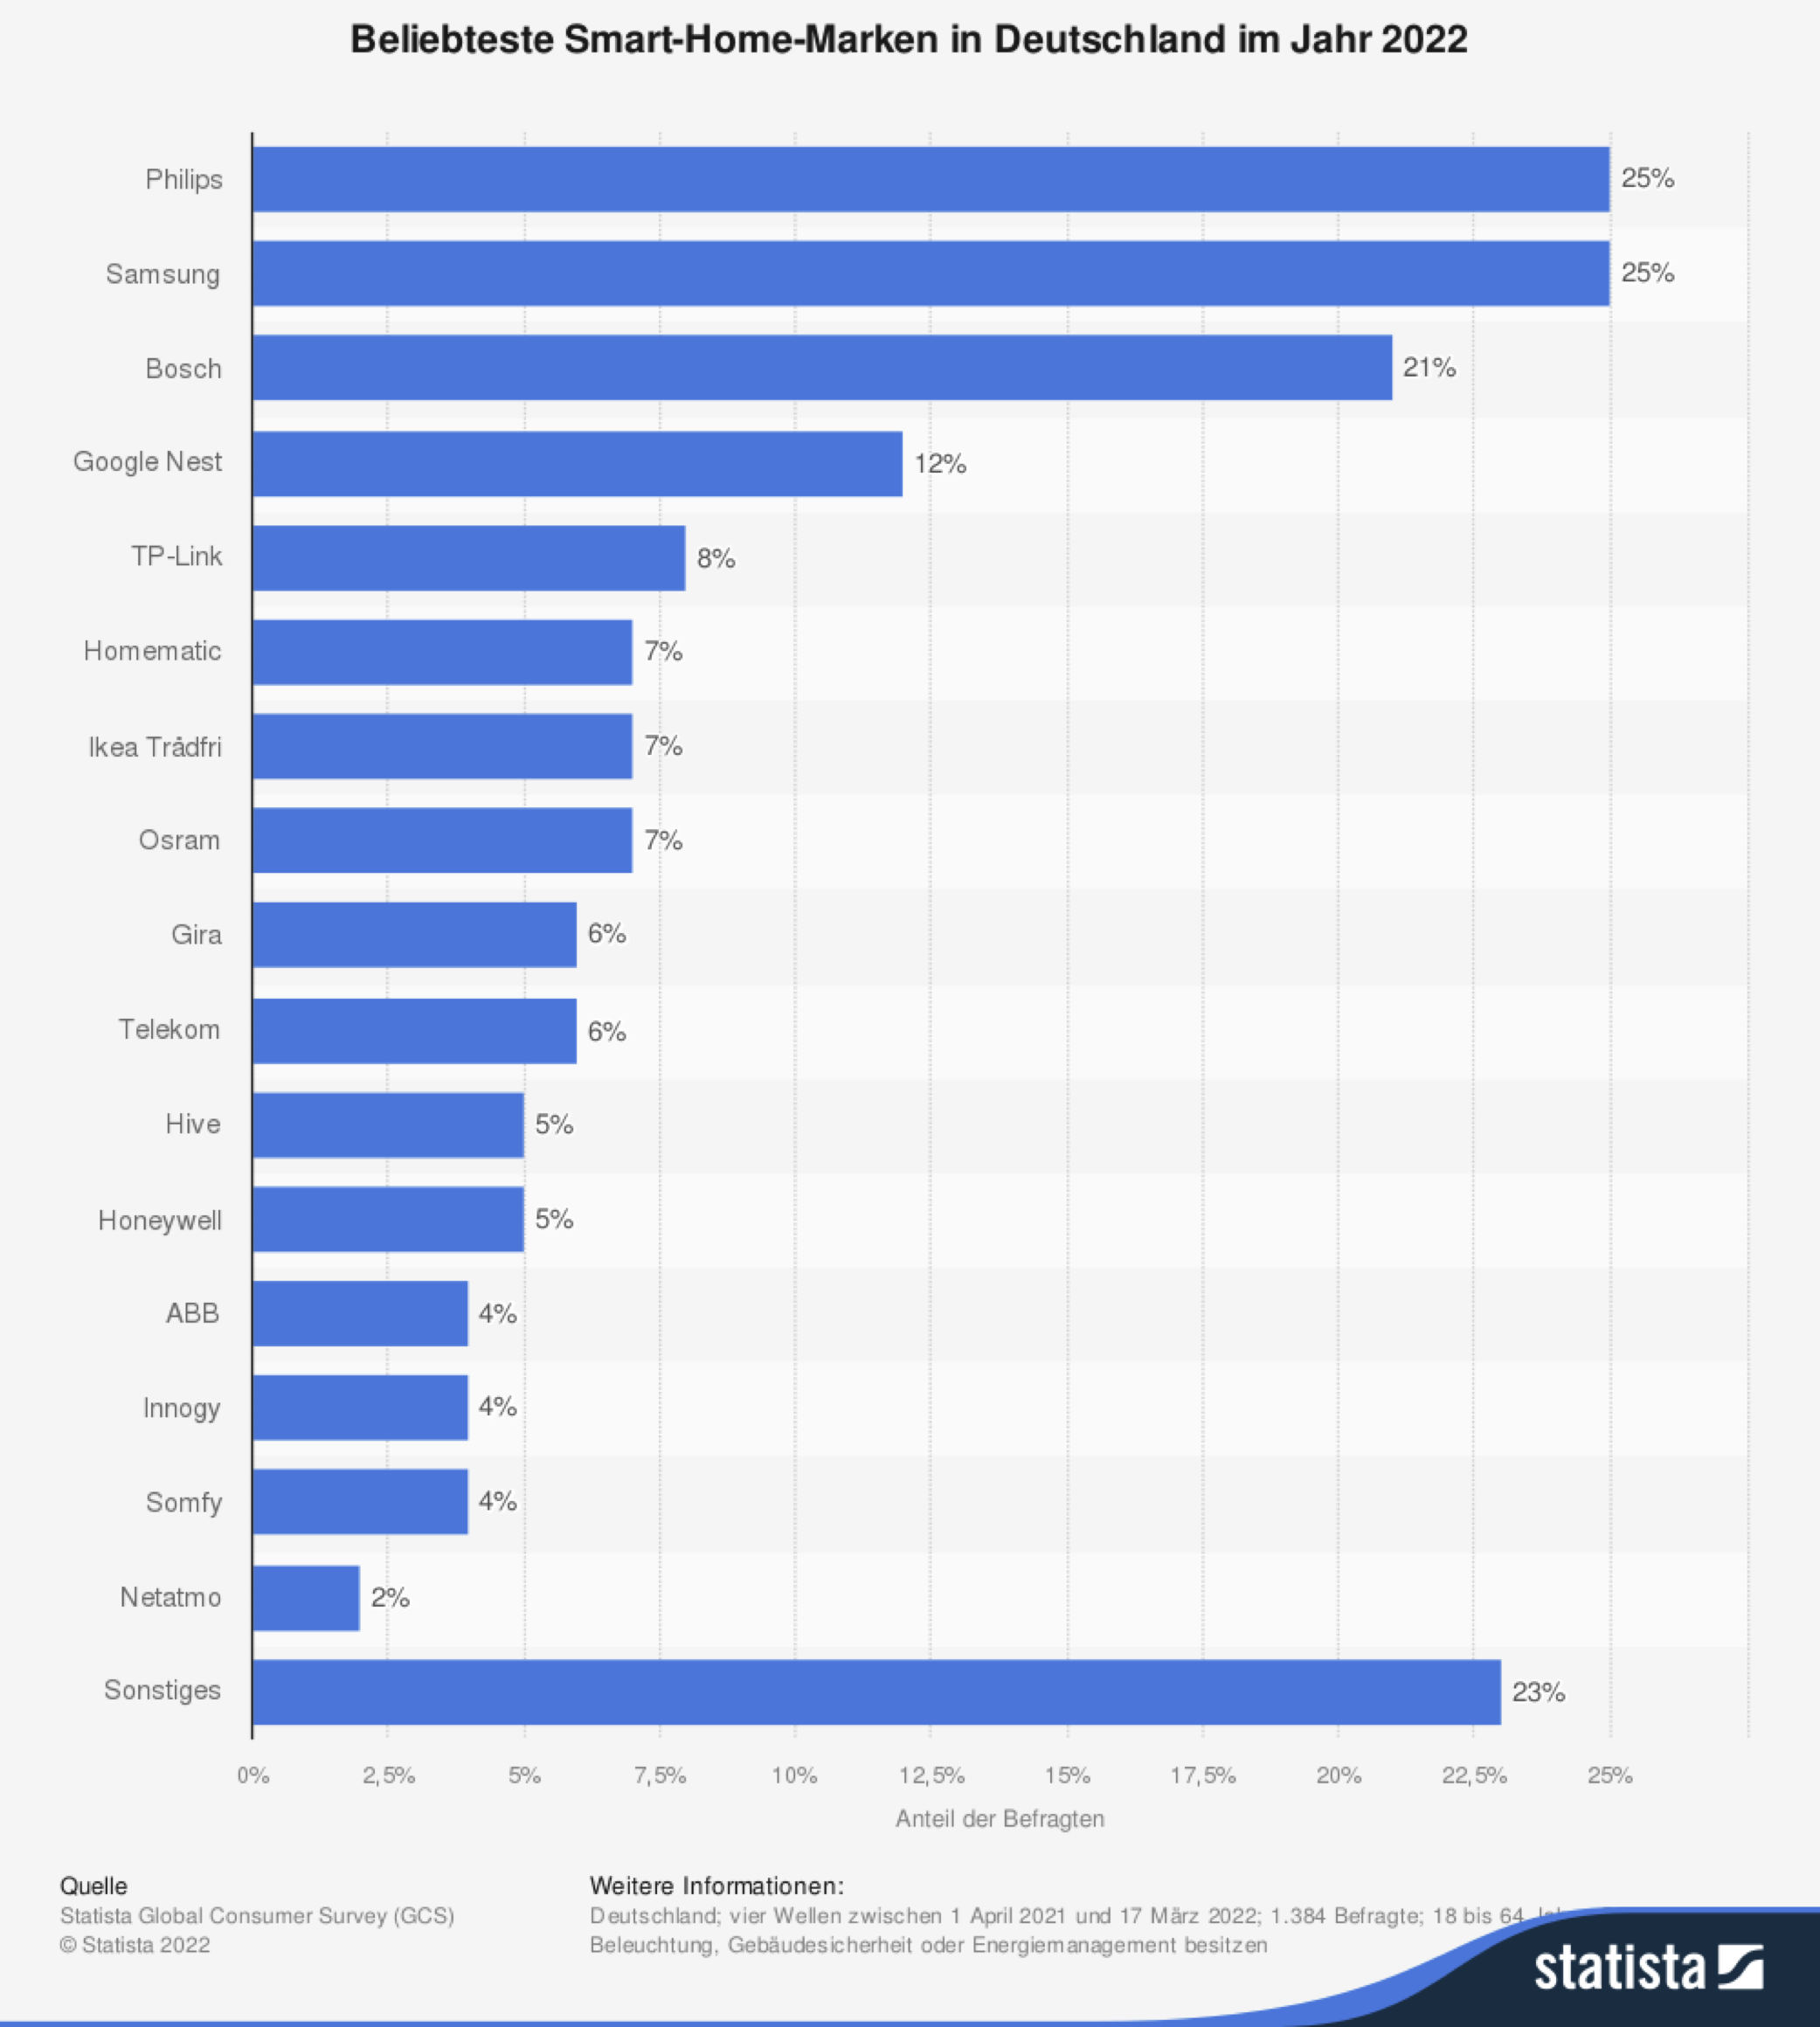
\includegraphics[width=13.5cm,height=13.5cm,keepaspectratio]{chapter/9Anhang/beliebteste-smart-home-marken-in-deutschland-2022.png}
  %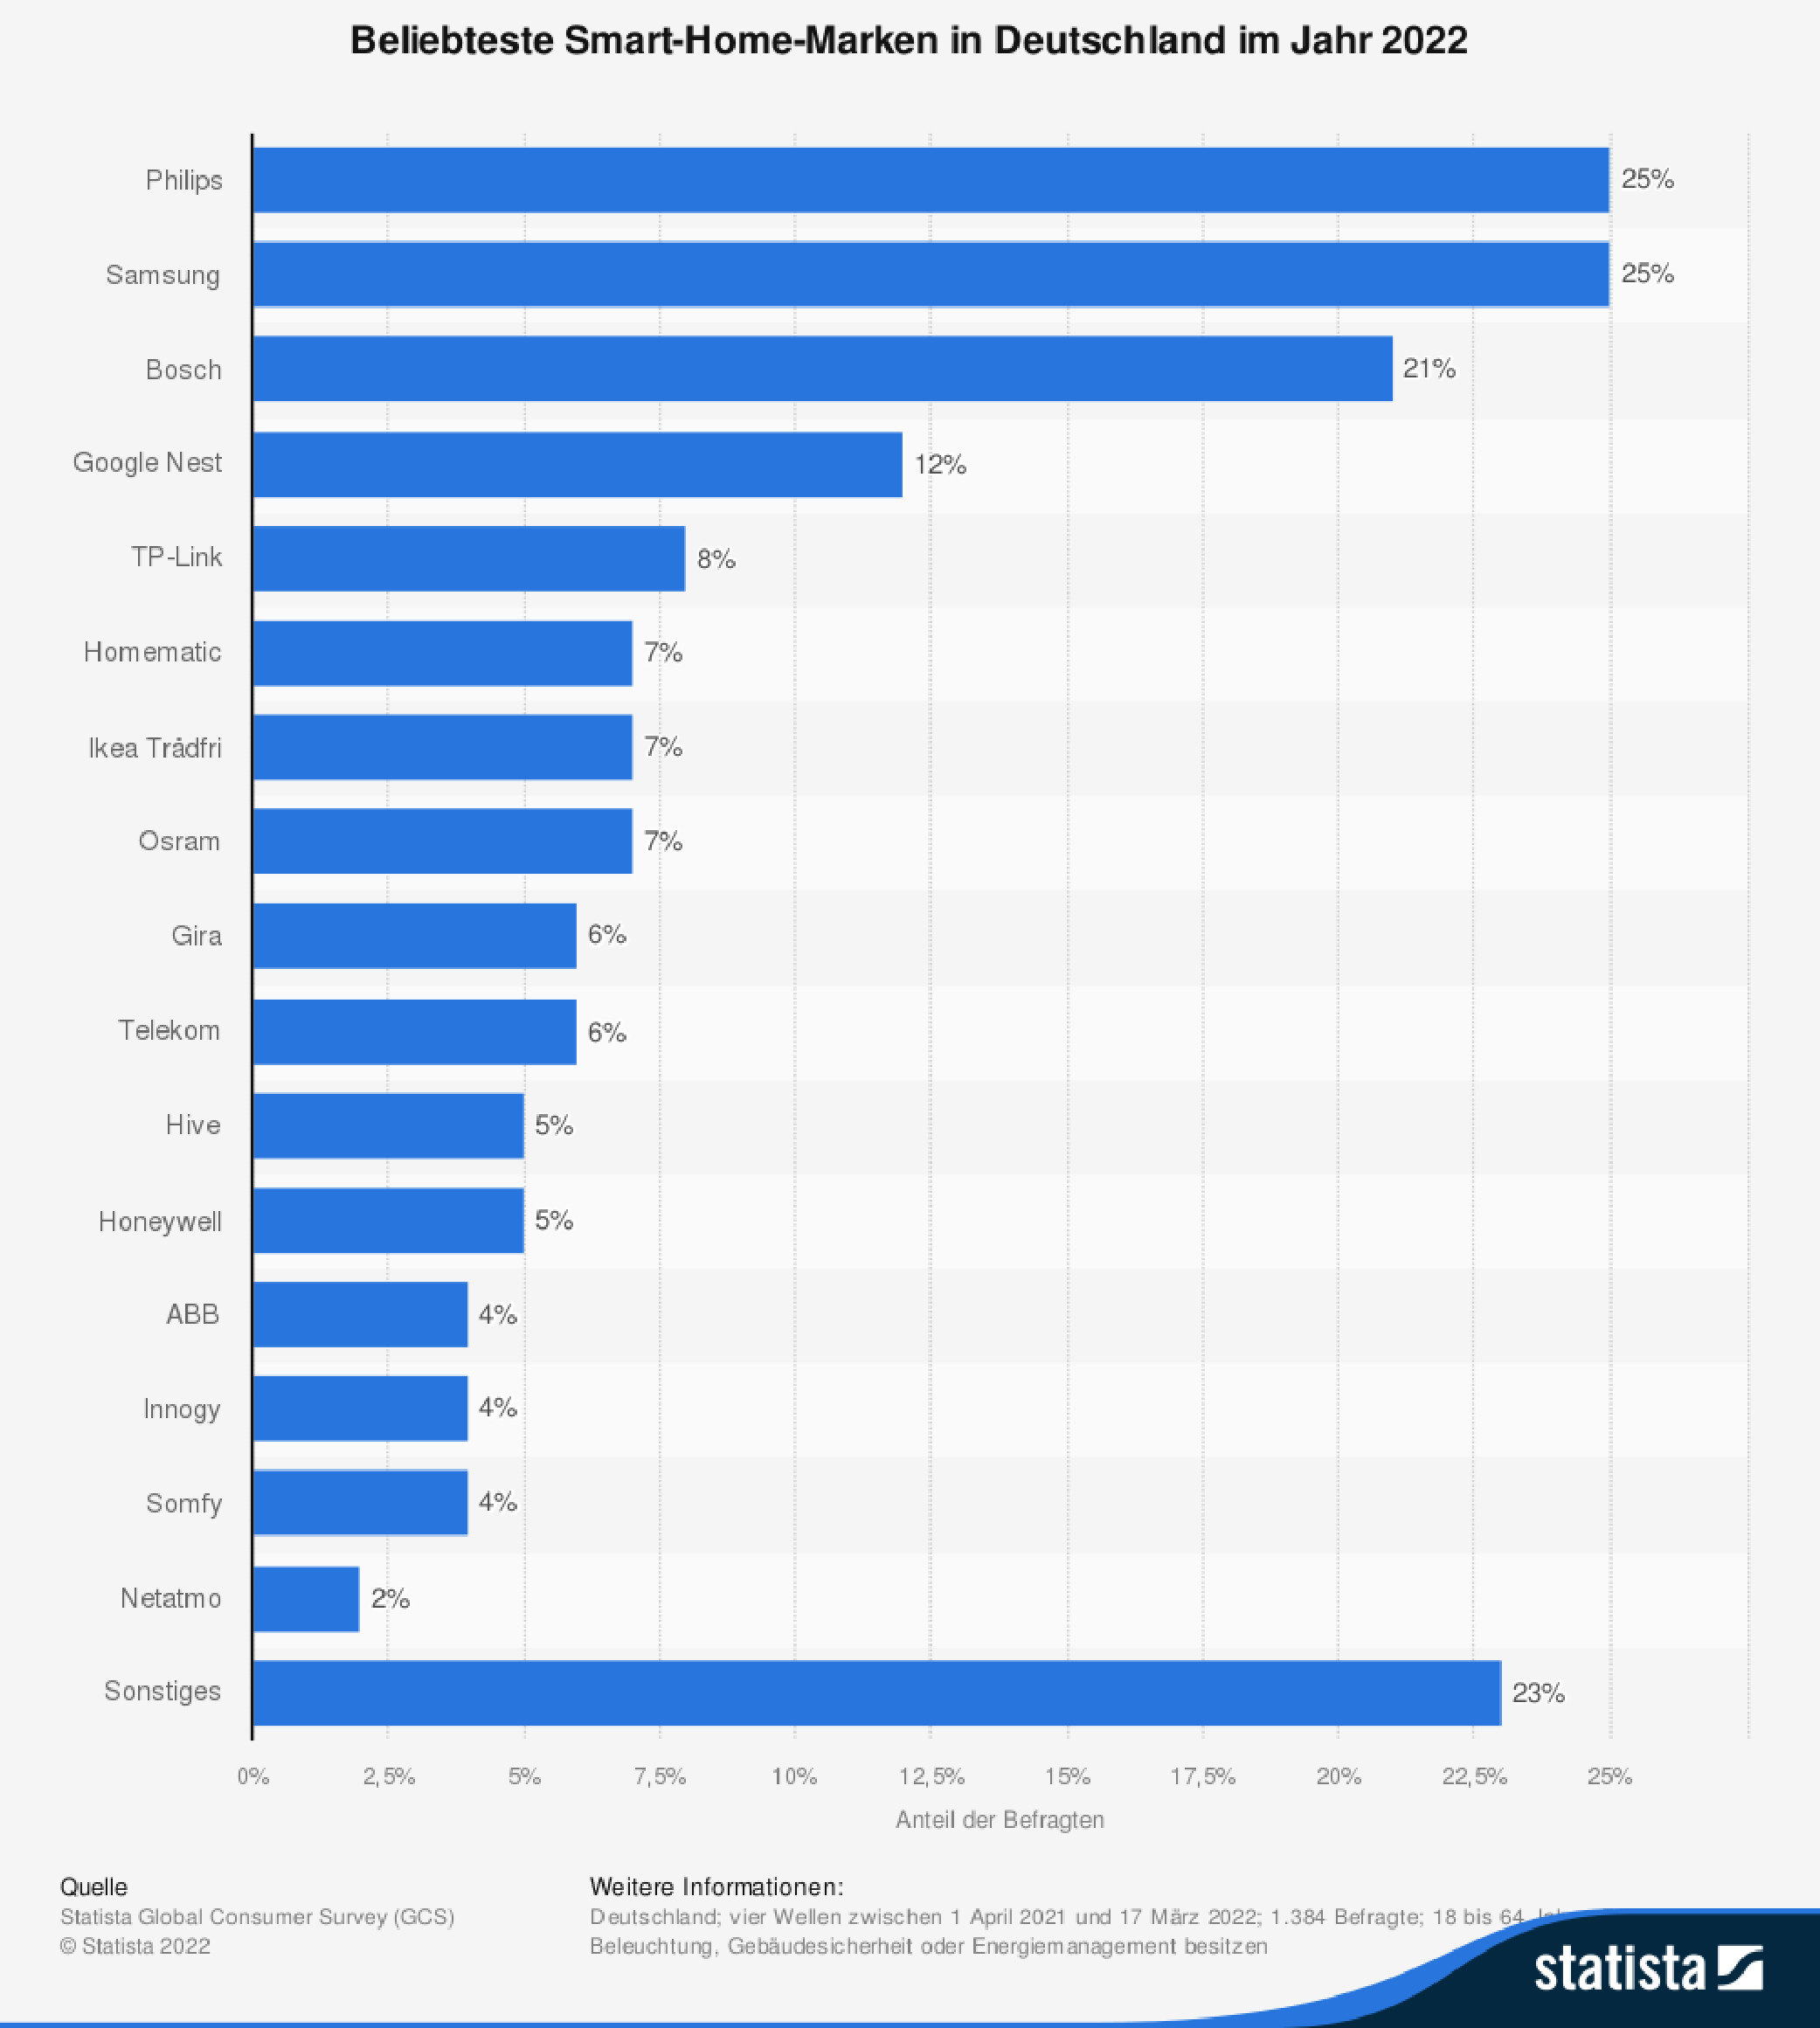
\includepdf[scale=0.65, pages=-, fitpaper=false]{chapter/9Anhang/beliebteste-smart-home-marken-in-deutschland-2022.pdf} %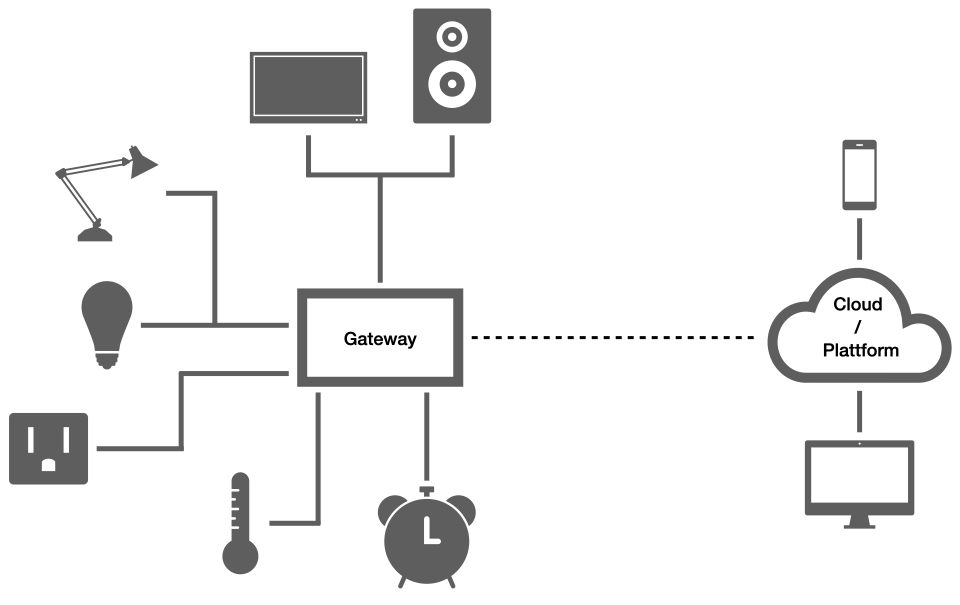
\includegraphics[width=13cm,height=13cm,keepaspectratio]{images/smart_home_connection.png}
  \caption{Umfrage der Statista GCS. Abgerufen am 22.05.2022}
  %\label{appendix:brandings}
\end{figure}

\chapter{}
\label{appendix:persona}
\begin{landscape}
  \AddToShipoutPictureBG*{%
  \AtPageLowerLeft{%
    \raisebox{\dimexpr.5\paperheight-.5\height}{%
      \makebox[.9\paperwidth][r]{%
        \rotatebox{90}
        {\thepage}
      }% \makebox
    }% \raisebox
  }% \AtPageCenter
}% \AddToShipoutPictureBG*
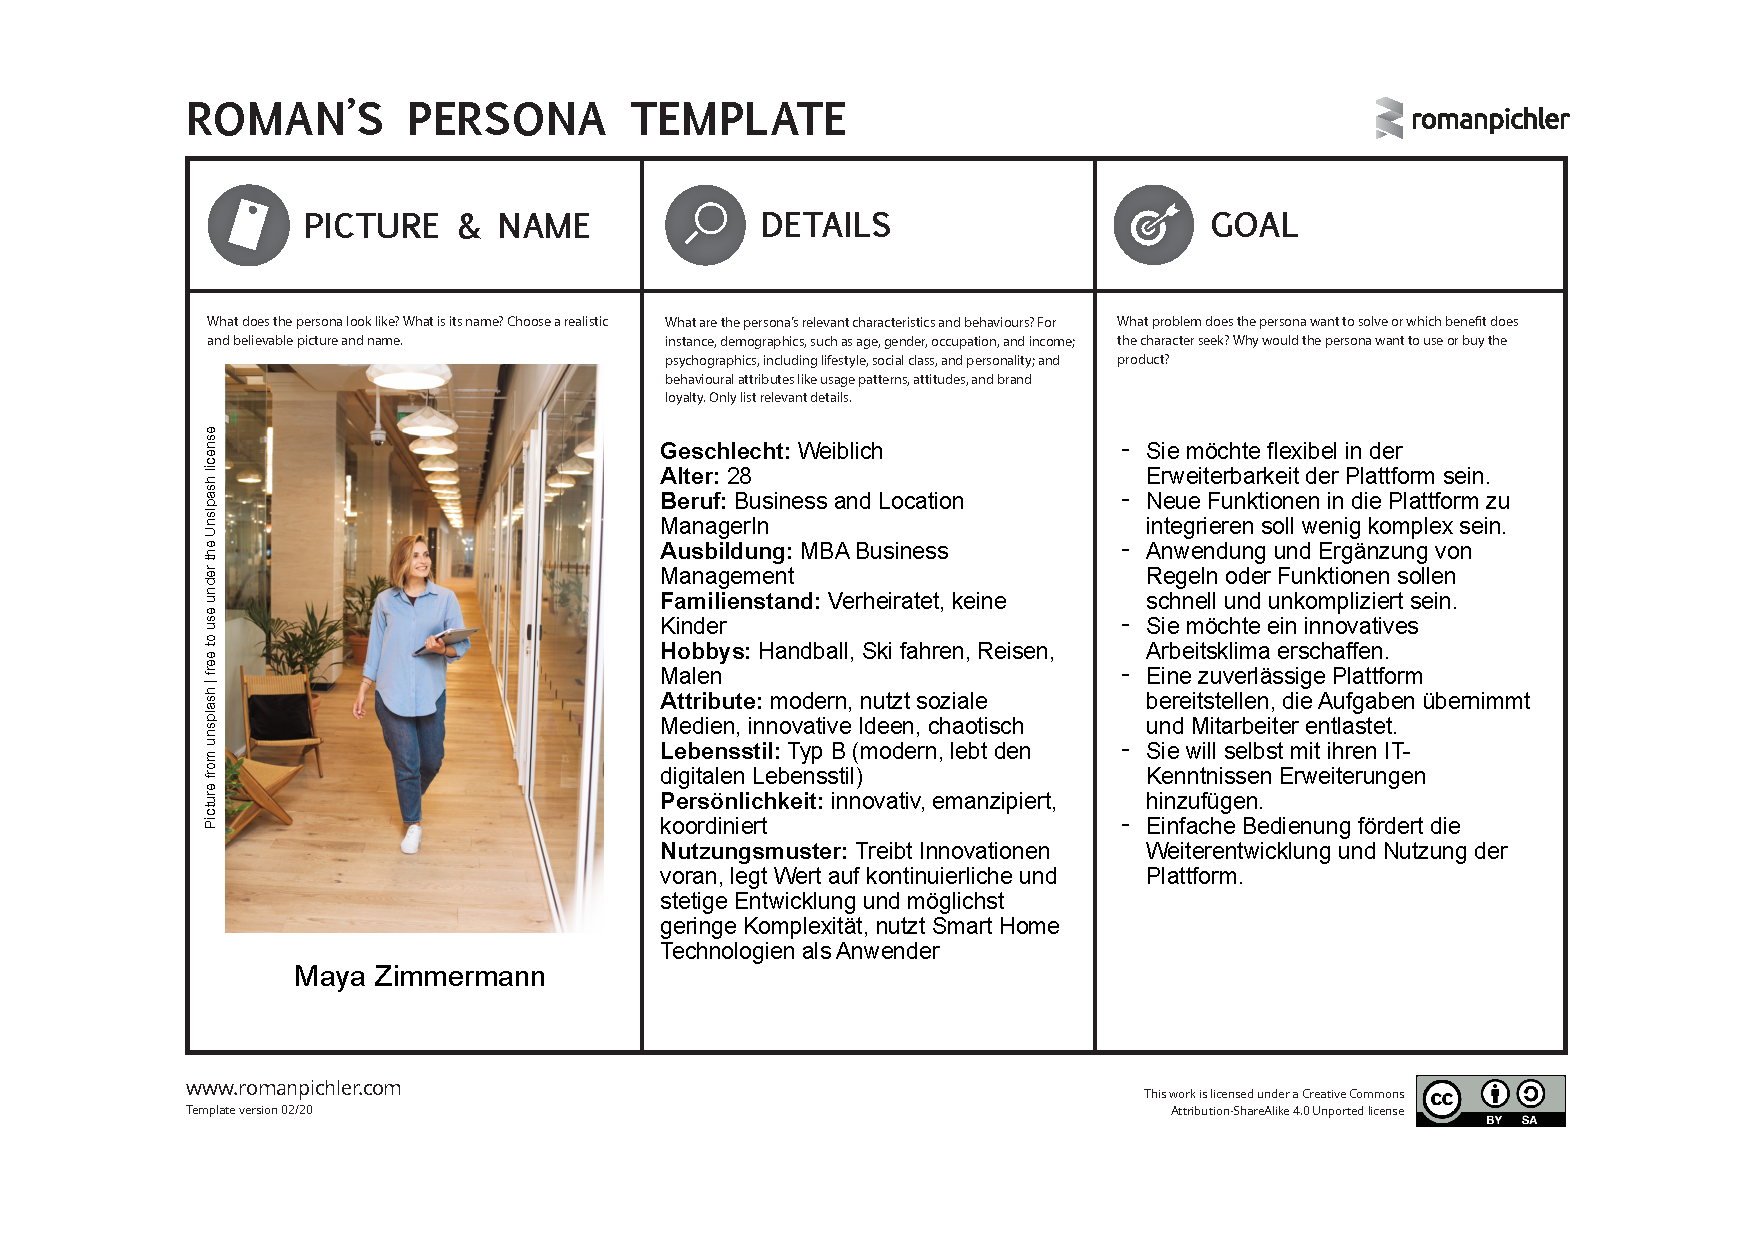
\includepdf[scale=0.75, pages=-, angle=90, fitpaper]{chapter/9Anhang/Persona-1_MA.pdf}
\end{landscape}
\begin{landscape}
  \AddToShipoutPictureBG*{%
  \AtPageLowerLeft{%
    \raisebox{\dimexpr.5\paperheight-.5\height}{%
      \makebox[.9\paperwidth][r]{%
        \rotatebox{90}
        {\thepage}
      }% \makebox
    }% \raisebox
  }% \AtPageCenter
}% \AddToShipoutPictureBG*
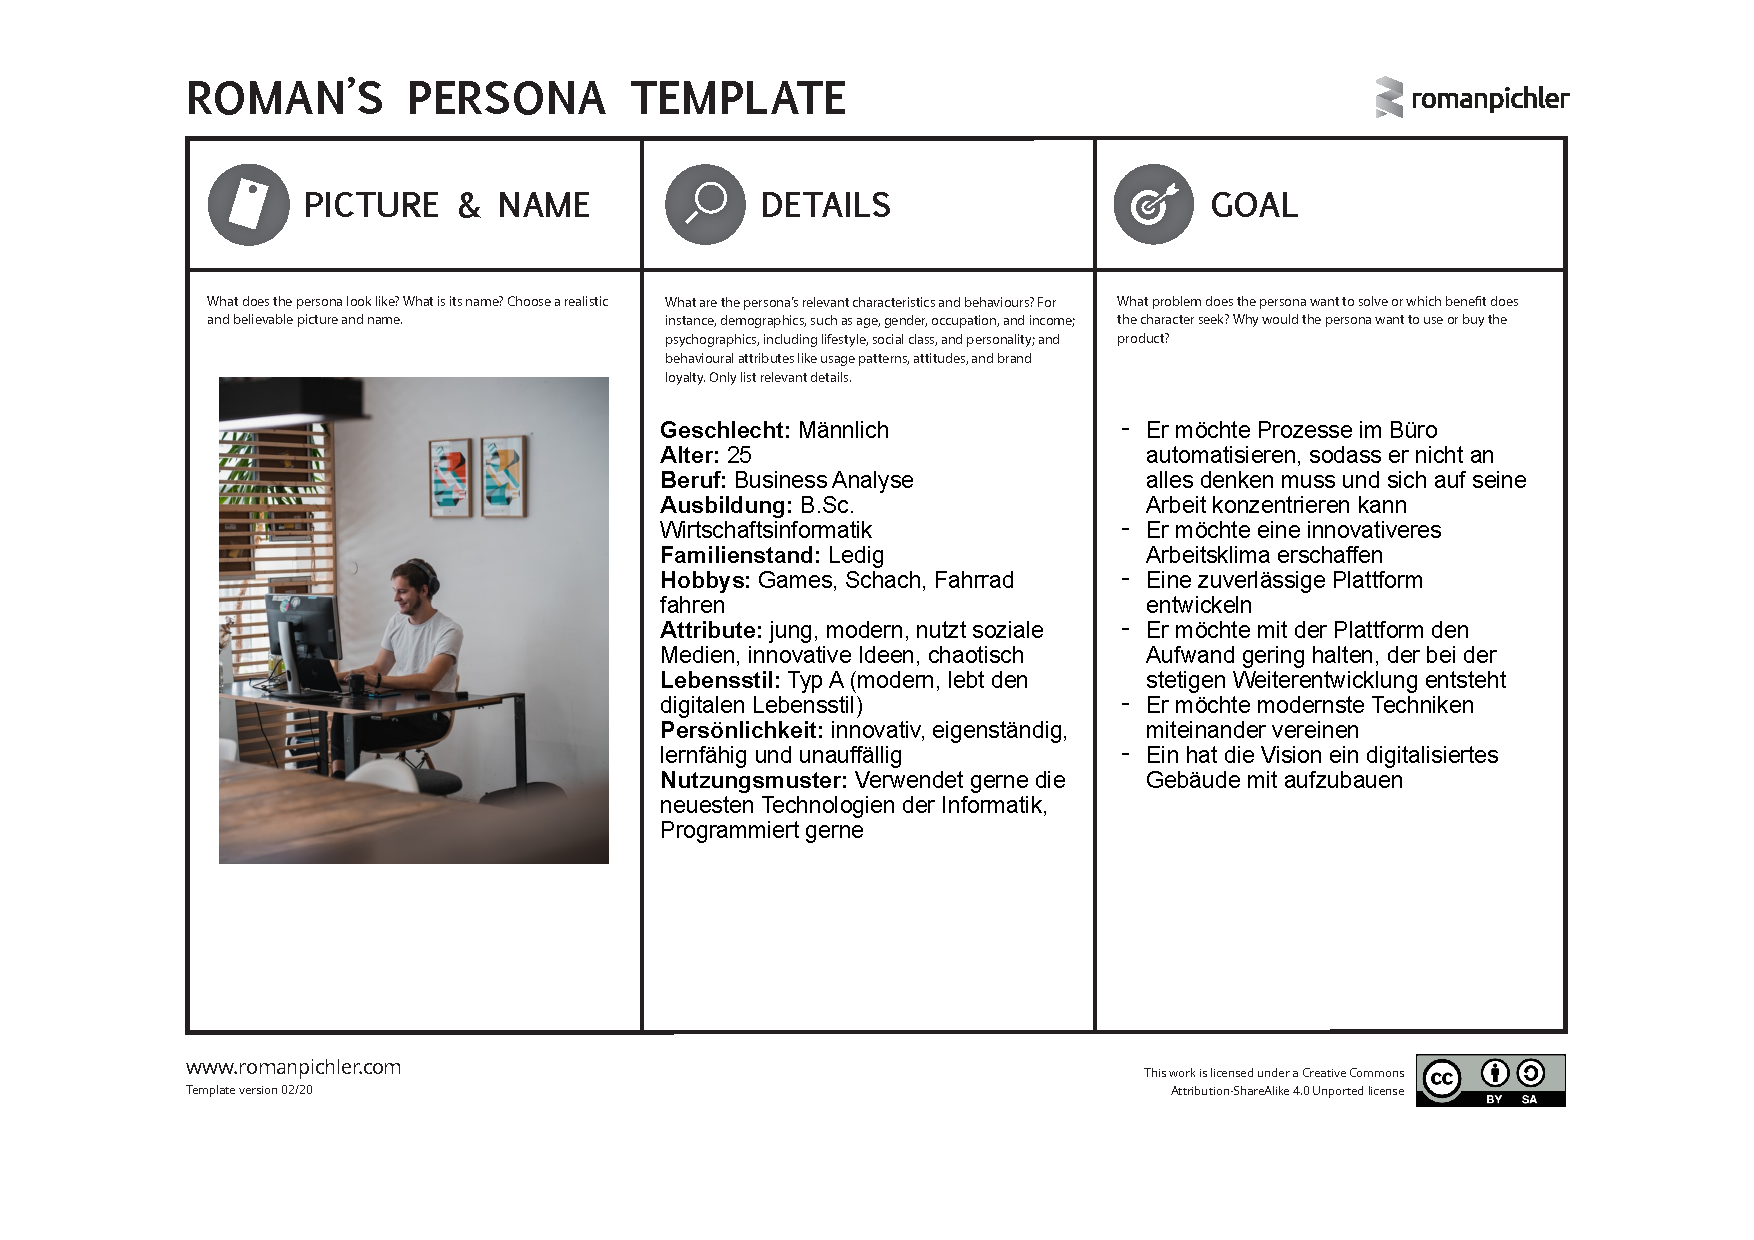
\includepdf[scale=0.75, pages=-, angle=90, fitpaper]{chapter/9Anhang/Persona-2_MA.pdf}
\end{landscape}
\begin{landscape}
  \AddToShipoutPictureBG*{%
  \AtPageLowerLeft{%
    \raisebox{\dimexpr.5\paperheight-.5\height}{%
      \makebox[.9\paperwidth][r]{%
        \rotatebox{90}
        {\thepage}
      }% \makebox
    }% \raisebox
  }% \AtPageCenter
}% \AddToShipoutPictureBG*
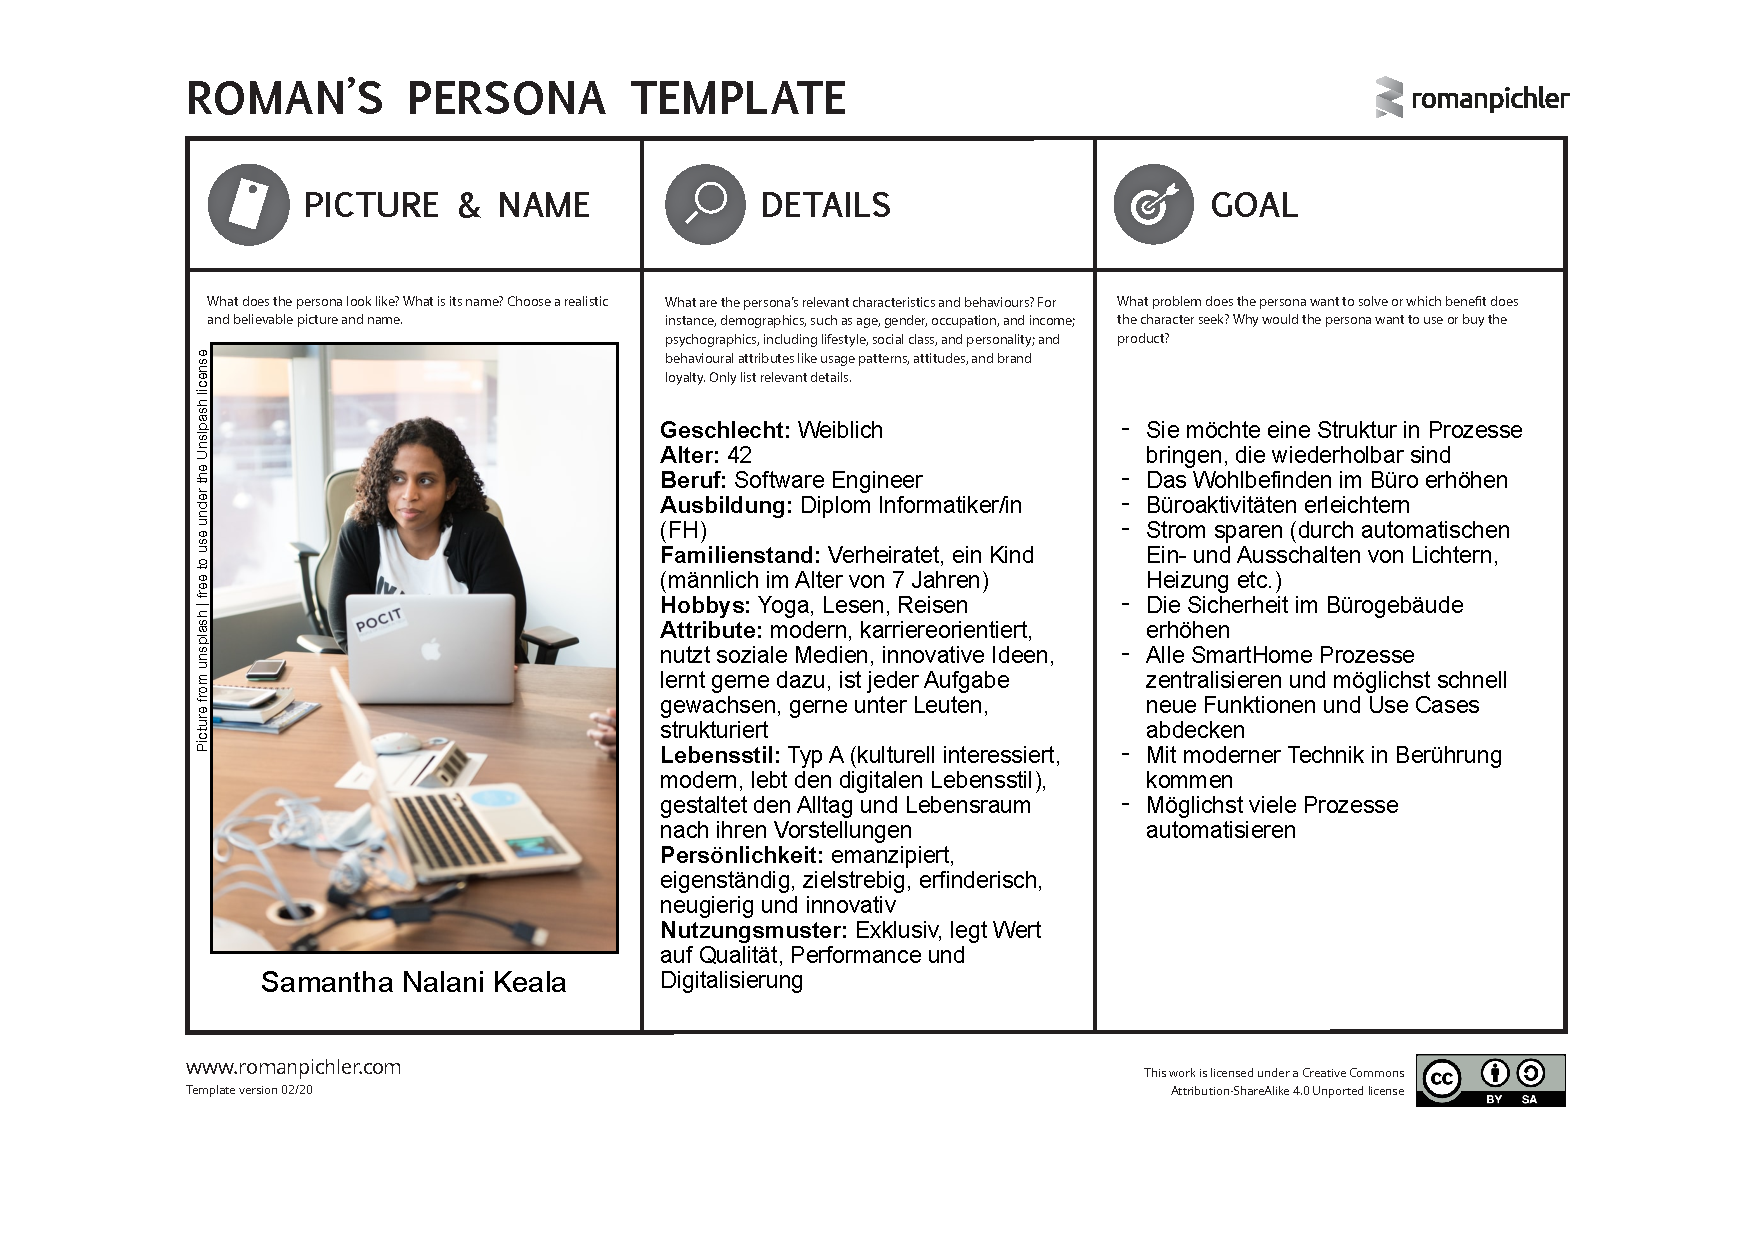
\includepdf[scale=0.75, angle=90, pages=-, fitpaper]{chapter/9Anhang/Persona-3_MA.pdf}
\end{landscape}

\chapter{}
\label{appendix:user-story-uc1}
%\section*{Use Case 1 - Check-in mit einem Service-Roboter}
\subsection*{Aufgabenbeschreibung UC 1}
\begin{table}[hbt!]
    \begin{center}
        \begin{tabular}{| p{3cm} | p{12.75cm} | }
            \hline
                \textbf{Task:} & \textbf{Begrüßung / Check-In von Member und Gästen} \\
            \hline
                \textbf{Ziel:} & Einen Member (Mitarbeiter) oder einen Gast in der Lokation mit einem Service-Roboter zu begrüßen, wenn dieser eintreten möchte. Nach der Begrüßung findet der Check-In statt, bei dem der Member seinem Platz zugewiesen und der Gast zu seinem Ansprechpartner geleitet wird. \\
            \hline
                \textbf{Eingriffs-möglichkeiten:} & Auswahl der Situation, Interaktion mit dem Service-Roboter (Informieren, Begleiten). \\
            \hline
                \textbf{Ursachen:} & Terminbuchung, Anmeldung, Klingeln an der Tür, Authentifizierung / Authentisierung an der Tür mittels Biometrische Eingangskontrolle. \\
            \hline
                \textbf{Priorität:} & Hoch \\
            \hline
                \textbf{Durchführungs-profil:} & Nach Anmeldung oder Eintritt eines Gastes oder Members, Unterbrechungen möglich (Verbindungsfehler, Fehlerhafte Abfrage der Verfügbarkeiten von Platzreservierungen), mittlere Komplexität. \\ 
            \hline
                \textbf{Vorbedingung:} & Platzbuchung / Reservierung und Einbuchung für ein Meeting fand im Vorfeld statt, Einverständniserklärung von den Personen liegt vor, Authentisierung über die Eingangskontrolle hat funktioniert / stattgefunden. \\
            \hline 
                \textbf{Info-In:} & Die Person, die eintreten will, ist durch die Buchung oder Authentisierung bekannt, Buchung ist registriert und kann abgerufen werden. \\
            \hline
                \textbf{Info-Out:} & Begrüßung Standardprotokoll mit Interaktionsmöglichkeiten und Kenntnis des Namens der Person, Check-In Informationen für die einzucheckende Person. \\
            \hline
                \textbf{Ressourcen:} & Service-Roboter, Eintrittskontrolle per Biometrischer Authentisierung, Buchung der Person abrufbar über die API. \\
            \hline
        \end{tabular}
    \end{center}
    \caption{Aufgabenbeschreibung UC 1 - Begrüßung / Check-in}
    \label{tab:checkIn}
\end{table}

%\subsection*{UC 1 - Beschreibung}
%    Steuerzentrale:
%    \begin{itemize}
%        \item Input: MQTT Nachricht von UC 1 (Verifizierung ok?, Name des Gastes / Members und Prozessanstoß (Check In))
%        \item Input: Terminregistrierung durch DoorJames (Übertragung der Termindaten) 
%        \item Output: Zu durchlaufender Prozess (CheckIn) und Name des Gastes / Members
%        \subItem (CheckIn) Genauer Begrüssungsprozess? Aktiv / Passiv 
%        \subsubItem Zuständigkeit Service-Roboter / Member / Gast / Steuerzentrale (Zentral / dezentral)
%        \subsubItem Begrüßungsprozess durch Service-Roboter selbst (Möglichkeiten sind im Service-Roboter implementiert) Steuerzentrale dient nur als Event-Auslöser 
%    \end{itemize}
	
%    Service-Roboter: 
%    \begin{itemize}
%        \item Input: MQTT (Prozess-Trigger durch Steuerzentrale und Name des Gastes / Members)
%        \item Input: Mitarbeiter lädt Kunde ein / Prepare / Nachweis der Platzbuchungssoftware
%        \item Output: (An Steuerzentrale) – Prozess erfolgreich abgeschlossen
%        \subItem Event-Möglichkeiten werden von Service-Roboter direkt verarbeitet. (Interaktion mit Gast, Ausrichten mit Hilfe Objekterkennung zur Person) 
%        \subItem Event-Möglichkeiten: 
%        \subsubItem Kunde: 
%        \subsubsubItem Begrüßen von Kunde und einchecken mit QR / Wenn eingeladen, Service-Roboter wartet schon vorher 5-15min vor der Tür
%        \subsubsubItem Zum Einladenden führen oder einen Call starten
%        \subsubItem Mitarbeiter: 
%        \subsubsubItem Anbieten eines Kaffees (zum Arbeitsplatz?) / oder zur Kaffee Maschine führen
%    \end{itemize}

\subsection*{UC 1 - User Story}
\textbf{Gast:}
\\
Als Gast möchte ich für den Zugang in das Gebäude ein Bild für den Anmeldeprozess hinterlegen können. Vor Ort möchte ich über die Kamera 
am Eingang mein Gesicht Authentisieren, bei nicht Hinterlegung eines Bildes bei der Anmeldung, möchte ich klingeln. Nach der 
Authentisierung bzw. nach Betätigung der Klingel soll sich die Tür öffnen. Beim Hineintreten in das Gebäude nehme ich einen Service-Roboter 
(Service-Roboter) wahr. Dieser begrüßt mich und startet eine Konversation mit mir. Er bietet mir an die Registrierung bzw. das Antreffen im Gebäude 
per QR Code über den Service-Roboter-Bildschirm durchzuführen. Somit werde ich als anwesend markiert und der Mitarbeiter, mit dem ich einen Termin 
habe, wird informiert. Nach erfolgreicher Registrierung führt mich der Service-Roboter zum Mitarbeiter mit dem ich einen Termin vereinbart habe.
\\
\linebreak
\textbf{Member:}\\

Als Member möchte ich die Buchung eines Arbeitsplatzes wahrnehmen können. Um in das Gebäude eintreten zu können, ist eine Authentifizierung durch 
die Gesichtserkennung oder das Abscannen der Chipkarte notwendig. Nach erfolgreicher Autorisierung werde ich von Service-Roboter bei Eintritt des Gebäudes 
begrüßt. Service-Roboter gibt mir den Arbeitsplatz bekannt und fragt, ob ich zum Platz begleitet werden soll. 
(oder Service-Roboter mir einen Kaffee an den Arbeitsplatz bringt.) -> (Erweiterung des Use Cases in Planung)
%Kunden zum Ausgangführen/Checkout anderer use case

\subsubsection*{Akzeptanzkriterien}
\begin{itemize}
    \item AK-01: Eine MQTT-Message mit dem Namen der Authentisierten Person wird empfangen.
    \item AK-02: Die MQTT-Message wird gelesen und mittels den Informationen können Abfragen an die DoorJames API erfolgen.
    \item AK-03: Informationen der DoorJames API werden empfangen und können weiterverarbeitet werden. 
    \item AK-04: Die benötigten Informationen können an den Service-Roboter (Temi) weitergeleitet werden.
    \item Ak-05: Eine MQTT-Message wird empfangen, sobald der Service-Roboter alle Tasks (ToDo's)  des Prozesses abgearbeitet hat. 
\end{itemize}

\section*{Use Case 1 - Check-in mit einem Service-Roboter}
\subsection*{Aufgabenbeschreibung UC 1}
\begin{table}[hbt!]
    \begin{center}
        \begin{tabular}{| p{3cm} | p{12.75cm} | }
            \hline
                \textbf{Task:} & \textbf{Begrüßung / Check-In von Member und Gästen} \\
            \hline
                \textbf{Ziel:} & Einen Member (Mitarbeiter) oder einen Gast in der Lokation mit einem Service-Roboter zu begrüßen, wenn dieser eintreten möchte. Nach der Begrüßung findet der Check-In statt, bei dem der Member seinem Platz zugewiesen und der Gast zu seinem Ansprechpartner geleitet wird. \\
            \hline
                \textbf{Eingriffs-möglichkeiten:} & Auswahl der Situation, Interaktion mit dem Service-Roboter (Informieren, Begleiten). \\
            \hline
                \textbf{Ursachen:} & Terminbuchung, Anmeldung, Klingeln an der Tür, Authentifizierung / Authentisierung an der Tür mittels Biometrische Eingangskontrolle. \\
            \hline
                \textbf{Priorität:} & Hoch \\
            \hline
                \textbf{Durchführungs-profil:} & Nach Anmeldung oder Eintritt eines Gastes oder Members, Unterbrechungen möglich (Verbindungsfehler, Fehlerhafte Abfrage der Verfügbarkeiten von Platzreservierungen), mittlere Komplexität. \\ 
            \hline
                \textbf{Vorbedingung:} & Platzbuchung / Reservierung und Einbuchung für ein Meeting fand im Vorfeld statt, Einverständniserklärung von den Personen liegt vor, Authentisierung über die Eingangskontrolle hat funktioniert / stattgefunden. \\
            \hline 
                \textbf{Info-In:} & Die Person, die eintreten will, ist durch die Buchung oder Authentisierung bekannt, Buchung ist registriert und kann abgerufen werden. \\
            \hline
                \textbf{Info-Out:} & Begrüßung Standardprotokoll mit Interaktionsmöglichkeiten und Kenntnis des Namens der Person, Check-In Informationen für die einzucheckende Person. \\
            \hline
                \textbf{Ressourcen:} & Service-Roboter, Eintrittskontrolle per Biometrischer Authentisierung, Buchung der Person abrufbar über die API. \\
            \hline
        \end{tabular}
    \end{center}
    \caption{Aufgabenbeschreibung UC 1 - Begrüßung / Check-in}
    \label{tab:checkIn}
\end{table}

%\subsection*{UC 1 - Beschreibung}
%    Steuerzentrale:
%    \begin{itemize}
%        \item Input: MQTT Nachricht von UC 1 (Verifizierung ok?, Name des Gastes / Members und Prozessanstoß (Check In))
%        \item Input: Terminregistrierung durch DoorJames (Übertragung der Termindaten) 
%        \item Output: Zu durchlaufender Prozess (CheckIn) und Name des Gastes / Members
%        \subItem (CheckIn) Genauer Begrüssungsprozess? Aktiv / Passiv 
%        \subsubItem Zuständigkeit Service-Roboter / Member / Gast / Steuerzentrale (Zentral / dezentral)
%        \subsubItem Begrüßungsprozess durch Service-Roboter selbst (Möglichkeiten sind im Service-Roboter implementiert) Steuerzentrale dient nur als Event-Auslöser 
%    \end{itemize}
	
%    Service-Roboter: 
%    \begin{itemize}
%        \item Input: MQTT (Prozess-Trigger durch Steuerzentrale und Name des Gastes / Members)
%        \item Input: Mitarbeiter lädt Kunde ein / Prepare / Nachweis der Platzbuchungssoftware
%        \item Output: (An Steuerzentrale) – Prozess erfolgreich abgeschlossen
%        \subItem Event-Möglichkeiten werden von Service-Roboter direkt verarbeitet. (Interaktion mit Gast, Ausrichten mit Hilfe Objekterkennung zur Person) 
%        \subItem Event-Möglichkeiten: 
%        \subsubItem Kunde: 
%        \subsubsubItem Begrüßen von Kunde und einchecken mit QR / Wenn eingeladen, Service-Roboter wartet schon vorher 5-15min vor der Tür
%        \subsubsubItem Zum Einladenden führen oder einen Call starten
%        \subsubItem Mitarbeiter: 
%        \subsubsubItem Anbieten eines Kaffees (zum Arbeitsplatz?) / oder zur Kaffee Maschine führen
%    \end{itemize}

\subsection*{UC 1 - User Story}
\textbf{Gast:}
\\
Als Gast möchte ich für den Zugang in das Gebäude ein Bild für den Anmeldeprozess hinterlegen können. Vor Ort möchte ich über die Kamera 
am Eingang mein Gesicht Authentisieren, bei nicht Hinterlegung eines Bildes bei der Anmeldung, möchte ich klingeln. Nach der 
Authentisierung, bzw. nach Betätigung der Klingel soll sich die Tür öffnen. Beim Hineintreten in das Gebäude nehme ich einen Service-Roboter 
(Service-Roboter) wahr. Dieser begrüßt mich und startet eine Konversation mit mir. Er bietet mir an die Registrierung, bzw. das Antreffen im Gebäude 
per QR Code über den Service-Roboter-Bildschirm durchzuführen. Somit werde ich als anwesend markiert und der Mitarbeiter, mit dem ich einen Termin 
habe, wird informiert. Nach erfolgreicher Registrierung führt mich der Service-Roboter zum Mitarbeiter mit dem ich einen Termin vereinbart habe.
\\
\linebreak
\textbf{Member:}\\

Als Member möchte ich die Buchung eines Arbeitsplatzes wahrnehmen können. Um in das Gebäude eintreten zu können, ist eine Authentifizierung durch 
die Gesichtserkennung oder das Abscannen der Chipkarte notwendig. Nach erfolgreicher Autorisierung werde ich von Service-Roboter bei Eintritt des Gebäudes 
begrüßt. Service-Roboter gibt mir den Arbeitsplatz bekannt und fragt, ob ich zum Platz begleitet werden soll. 
(oder Service-Roboter mir einen Kaffee an den Arbeitsplatz bringt.) -> (Erweiterung des Use Cases in Planung)
%Kunden zum Ausgangführen/Checkout anderer use case

\subsubsection*{Akzeptanzkriterien}
\begin{itemize}
    \item AK-01: Eine MQTT-Message mit dem Namen der Authentisierten Person wird empfangen.
    \item AK-02: Die MQTT-Message wird gelesen und mittels den Informationen können Abfragen an die DoorJames API erfolgen.
    \item AK-03: Informationen der DoorJames API werden empfangen und können weiterverarbeitet werden. 
    \item AK-04: Die benötigten Informationen können an den Service-Roboter (Temi) weitergeleitet werden.
    \item Ak-05: Eine MQTT-Message wird empfangen, sobald der Service-Roboter alle Tasks (ToDo's)  des Prozesses abgearbeitet hat. 
\end{itemize}

\begin{landscape}
  \AddToShipoutPictureBG*{%
  \AtPageLowerLeft{%
    \raisebox{\dimexpr.5\paperheight-.5\height}{%
      \makebox[.9\paperwidth][r]{%
        \rotatebox{90}
        {\thepage}
      }% \makebox
    }% \raisebox
  }% \AtPageCenter
}% \AddToShipoutPictureBG*
  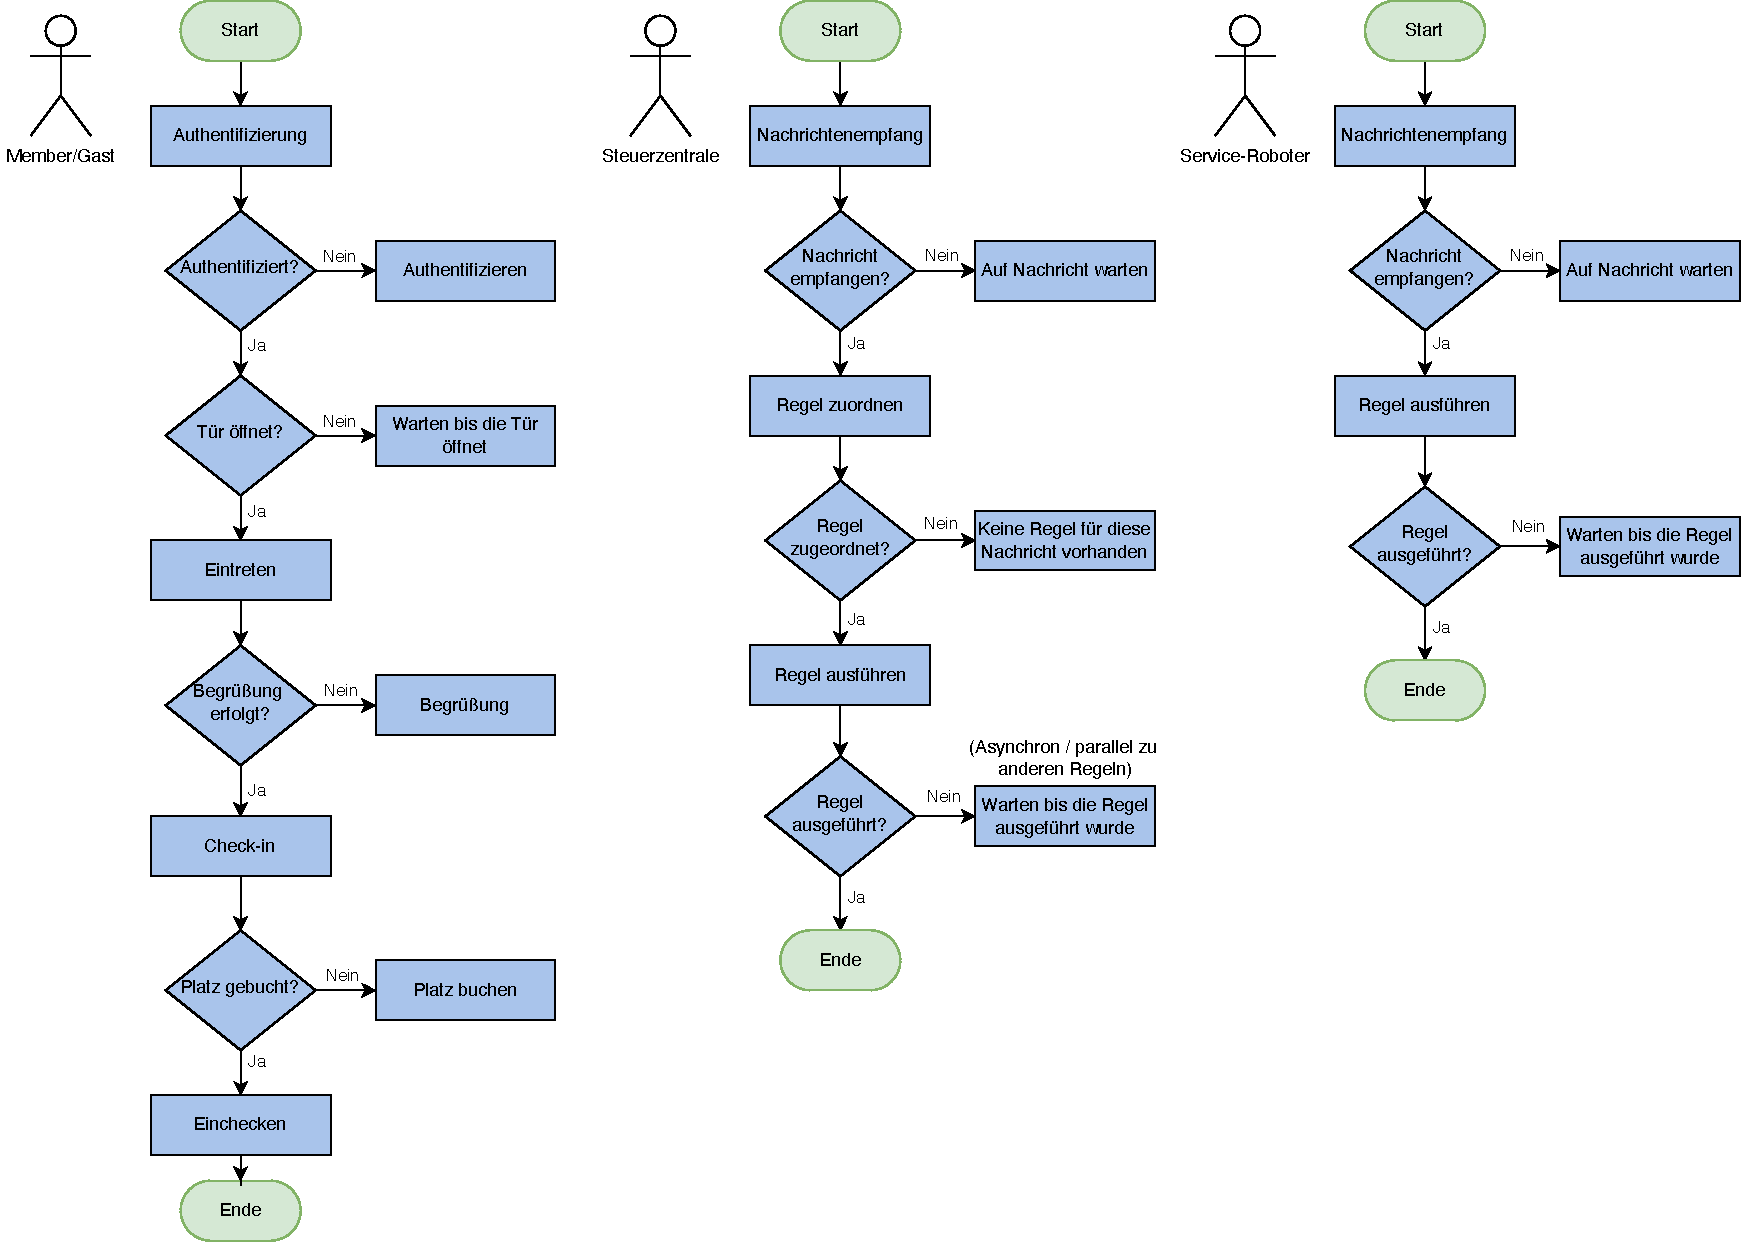
\includepdf[scale=0.75, pages=-, angle=90, fitpaper]{images/UC1_Ablaufdiagramm_Sichtweisen.pdf}
\end{landscape}
\pagebreak
\label{appendix:user-story-uc2}
%\section*{Use Case 2 - Notfall-Evakuierung}
\begin{table}[hbt!]
    \begin{center}
        \begin{tabular}{| p{3cm} | p{12.75cm} | }
            \hline
                \textbf{Task:} & \textbf{Begrüßung / Check-In von Member und Gästen} \\
            \hline
                \textbf{Ziel:} & Einen Notfall zu erkennen und darauf hin alle Member und Gäste, die sich im Büro befinden, informieren und bitten das Gebäude zu verlassen. \\
            \hline
                \textbf{Eingriffs-möglichkeiten:} & Keine, (Evtl. direkte Interaktion mit dem Service-Roboter). \\
            \hline
                \textbf{Ursachen:} & Aktivierung des Sensors durch äußerliche Einwirkung. \\
            \hline
                \textbf{Priorität:} & Hoch \\
            \hline
                \textbf{Durchführungs-profil:} & nach Meldung eines Notfalls durch Sensoren und Melder \\ 
            \hline
                \textbf{Vorbedingung:} & Ein Melder kann Nachrichten veröffentlichen, Topics für die Melder und Empfänger sind definiert. \\
            \hline 
                \textbf{Info-In:} & Meldung eines Sensors (Melder) über einen Notfall (Rauch, Feuer, Wasser, Gas). \\
            \hline
                \textbf{Info-Out:} & Kenntnis der gebuchten Plätze, Interaktionsmöglichkeiten mit dem Service-Roboter, Benachrichtigung bei Beendung des Prozesses. \\
            \hline
                \textbf{Ressourcen:} & Service-Roboter, Sensor (Rauch-, Feuer- oder Gas-Melder), Information über aktuelle Buchungen, Zuordnung von Positionen von Büroplätzen. \\
            \hline
        \end{tabular}
    \end{center}
    \caption{Aufgabenbeschreibung UC 2 - Notfall-Evakuierung}
    \label{tab:evacuation}
\end{table}

%\subsection*{UC 2 - Beschreibung}
%%    Steuerzentrale:
%    \begin{itemize}
%        \item Input: MQTT Nachricht angestoßen von einem Member (Aktion; Uhrzeit)
%        \item Input: DoorJames API - Gebuchte Büroplätze und Personen die einen Termin vor Ort registriert haben
%        \item -	Output: Zu durchlaufender Prozess (Evakuierung) und Name des Gastes / Members und Position der Plätze und Räume, die gebucht wurden. 
%    \end{itemize}
	
%    Service-Roboter: 
%    \begin{itemize}
%        \item Input: MQTT (Prozess-Trigger durch Steuerzentrale und Position gebuchter Plätze und Räume
%        \item Input: Objekterkennung (Personenerkennung) durch die Kamera
%        \item Output: (An Steuerzentrale) – Status / Prozess (erfolgreich/nicht erfolgreich) abgeschlossen
%        \item -> Event-Möglichkeiten werden von Service-Roboter direkt verarbeitet. (Interaktion mit Person, Anweisungen an die Person) 
%        \item -> Event-Möglichkeiten: 
%        \item --> Kunde, Gast & Member: 
%        \item ---> Alarmieren und bitten das Gebäude auf schnellstem Weg zu
%    \end{itemize}

\subsection*{UC 2 - User Story}
\textbf{Gast:}
\\
    Als Gast, Member und Manager möchte ich bei einem Notfall alarmiert werden. Bei eintretendem Fall möchte ich 
    Anweisungen, die zu beachten und umzusetzen sind, erhalten. Ebenso ist ein Hinweis zu den Notausgängen 
    sinnvoll und hilft bei der Flucht bzw. beim Verlassen des Gebäudes. Damit keine Personen im Büro 
    bleiben, ist eine Information über Anwesende von belangen. Der Member sollte die Möglichkeit haben, den 
    Service-Roboter aufzufordern nach Leuten zu rufen, die nicht in Sichtweite sind. Sobald alle Plätze 
    abgefahren sind bzw. durch den Service-Roboter keine Personen mehr erkannt werden, soll eine Benachrichtigung 
    erfolgen, dass alle aus dem Gebäude sind bzw. keine mehr gesichtet wurden. Diese Information hilft bei der 
    anschließenden Kontrolle über am Treffpunkt anwesender Personen. Abschließend soll ggf. Eine Information über die 
    Platzbuchungen gezeigt werden, damit bei der Kontrolle keine Fehler unterlaufen und keine Personen, die nicht 
    gesehen werden, vergessen werden.

\subsection*{Akzeptanzkriterien}
\begin{itemize}
    \item AK-01: Eine MQTT-Message des Rauchmelders (Sensors) wird von der Steuerzentrale empfangen.
    \item AK-02: Die MQTT-Message wird gelesen und Abfragen an die DoorJames API erfolgen (Abfrage der Personen zum Zeitpunk im Bürogebäude)
    \item AK-03: Informationen der DoorJames API werden empfangen und können weiterverarbeitet werden. 
    \item AK-04: Die benötigten Informationen können an den Service-Roboter (Temi) weitergeleitet werden.
    \item AK-05: Temi wird losgeschickt, um nach Personen im Gebäude zu suchen.
    \item AK-06: Die Steuerzenrale schickt eine SMS, E-Mail an die Gebäudeverantwortliche Person, dass ein Notfall losgetreten wurde.
    \item Ak-07: Eine MQTT-Message wird empfangen, sobald der Service-Roboter alle Tasks (ToDo's)  des Prozesses abgearbeitet hat. 
\end{itemize}
\section*{Use Case 2 - Notfall-Evakuierung}
\subsection*{Aufgabenbeschreibung UC 2}
\begin{table}[hbt!]
    \begin{center}
        \begin{tabular}{| p{3cm} | p{12.75cm} | }
            \hline
                \textbf{Task:} & \textbf{Begrüßung / Check-In von Member und Gästen} \\
            \hline
                \textbf{Ziel:} & Einen Notfall zu erkennen und darauf hin alle Member und Gäste, die sich im Büro befinden, informieren und bitten das Gebäude zu verlassen. \\
            \hline
                \textbf{Eingriffs-möglichkeiten:} & Keine, (Evtl. direkte Interaktion mit dem Service-Roboter). \\
            \hline
                \textbf{Ursachen:} & Aktivierung des Sensors durch äußerliche Einwirkung. \\
            \hline
                \textbf{Priorität:} & Hoch \\
            \hline
                \textbf{Durchführungs-profil:} & nach Meldung eines Notfalls durch Sensoren und Melder \\ 
            \hline
                \textbf{Vorbedingung:} & Ein Melder kann Nachrichten veröffentlichen, Topics für die Melder und Empfänger sind definiert. \\
            \hline 
                \textbf{Info-In:} & Meldung eines Sensors (Melder) über einen Notfall (Rauch, Feuer, Wasser, Gas). \\
            \hline
                \textbf{Info-Out:} & Kenntnis der gebuchten Plätze, Interaktionsmöglichkeiten mit dem Service-Roboter, Benachrichtigung bei Beendung des Prozesses. \\
            \hline
                \textbf{Ressourcen:} & Service-Roboter, Sensor (Rauch-, Feuer- oder Gas-Melder), Information über aktuelle Buchungen, Zuordnung von Positionen von Büroplätzen. \\
            \hline
        \end{tabular}
    \end{center}
    \caption{Aufgabenbeschreibung UC 2 - Notfall-Evakuierung}
    \label{tab:evacuation}
\end{table}

%\subsection*{UC 2 - Beschreibung}
%%    Steuerzentrale:
%    \begin{itemize}
%        \item Input: MQTT Nachricht angestoßen von einem Member (Aktion; Uhrzeit)
%        \item Input: DoorJames API - Gebuchte Büroplätze und Personen die einen Termin vor Ort registriert haben
%        \item -	Output: Zu durchlaufender Prozess (Evakuierung) und Name des Gastes / Members und Position der Plätze und Räume, die gebucht wurden. 
%    \end{itemize}
	
%    Service-Roboter: 
%    \begin{itemize}
%        \item Input: MQTT (Prozess-Trigger durch Steuerzentrale und Position gebuchter Plätze und Räume
%        \item Input: Objekterkennung (Personenerkennung) durch die Kamera
%        \item Output: (An Steuerzentrale) – Status / Prozess (erfolgreich/nicht erfolgreich) abgeschlossen
%        \item -> Event-Möglichkeiten werden von Service-Roboter direkt verarbeitet. (Interaktion mit Person, Anweisungen an die Person) 
%        \item -> Event-Möglichkeiten: 
%        \item --> Kunde, Gast & Member: 
%        \item ---> Alarmieren und bitten das Gebäude auf schnellstem Weg zu
%    \end{itemize}

\subsection*{UC 2 - User Story}
\textbf{Gast:}
\\
    Als Gast, Member und Manager möchte ich bei einem Notfall alarmiert werden. Bei eintretendem Fall möchte ich 
    Anweisungen, die zu beachten und umzusetzen sind, erhalten. Ebenso ist ein Hinweis zu den Notausgängen 
    sinnvoll und hilft bei der Flucht, bzw. beim Verlassen des Gebäudes. Damit keine Personen im Büro 
    bleiben, ist eine Information über Anwesende von belangen. Der Member sollte die Möglichkeit haben, den 
    Service-Roboter aufzufordern nach Leuten zu rufen, die nicht in Sichtweite sind. Sobald alle Plätze 
    abgefahren sind, bzw. durch den Service-Roboter keine Personen mehr erkannt werden, soll eine Benachrichtigung 
    erfolgen, dass alle aus dem Gebäude sind, bzw. keine mehr gesichtet wurden. Diese Information hilft bei der 
    anschließenden Kontrolle über am Treffpunkt anwesender Personen. Abschließend soll ggf. Eine Information über die 
    Platzbuchungen gezeigt werden, damit bei der Kontrolle keine Fehler unterlaufen und keine Personen, die nicht 
    gesehen werden, vergessen werden.

\subsection*{Akzeptanzkriterien}
\begin{itemize}
    \item AK-01: Eine MQTT-Message des Rauchmelders (Sensors) wird von der Steuerzentrale empfangen.
    \item AK-02: Die MQTT-Message wird gelesen und Abfragen an die DoorJames API erfolgen (Abfrage der Personen zum Zeitpunk im Bürogebäude)
    \item AK-03: Informationen der DoorJames API werden empfangen und können weiterverarbeitet werden. 
    \item AK-04: Die benötigten Informationen können an den Service-Roboter (Temi) weitergeleitet werden.
    \item AK-05: Temi wird losgeschickt, um nach Personen im Gebäude zu suchen.
    \item AK-06: Die Steuerzenrale schickt eine SMS, E-Mail an die Gebäudeverantwortliche Person, dass ein Notfall losgetreten wurde.
    \item Ak-07: Eine MQTT-Message wird empfangen, sobald der Service-Roboter alle Tasks (ToDo's)  des Prozesses abgearbeitet hat. 
\end{itemize}

\begin{landscape}
  \AddToShipoutPictureBG*{%
  \AtPageLowerLeft{%
    \raisebox{\dimexpr.5\paperheight-.5\height}{%
      \makebox[.9\paperwidth][r]{%
        \rotatebox{90}
        {\thepage}
      }% \makebox
    }% \raisebox
  }% \AtPageCenter
}% \AddToShipoutPictureBG*
  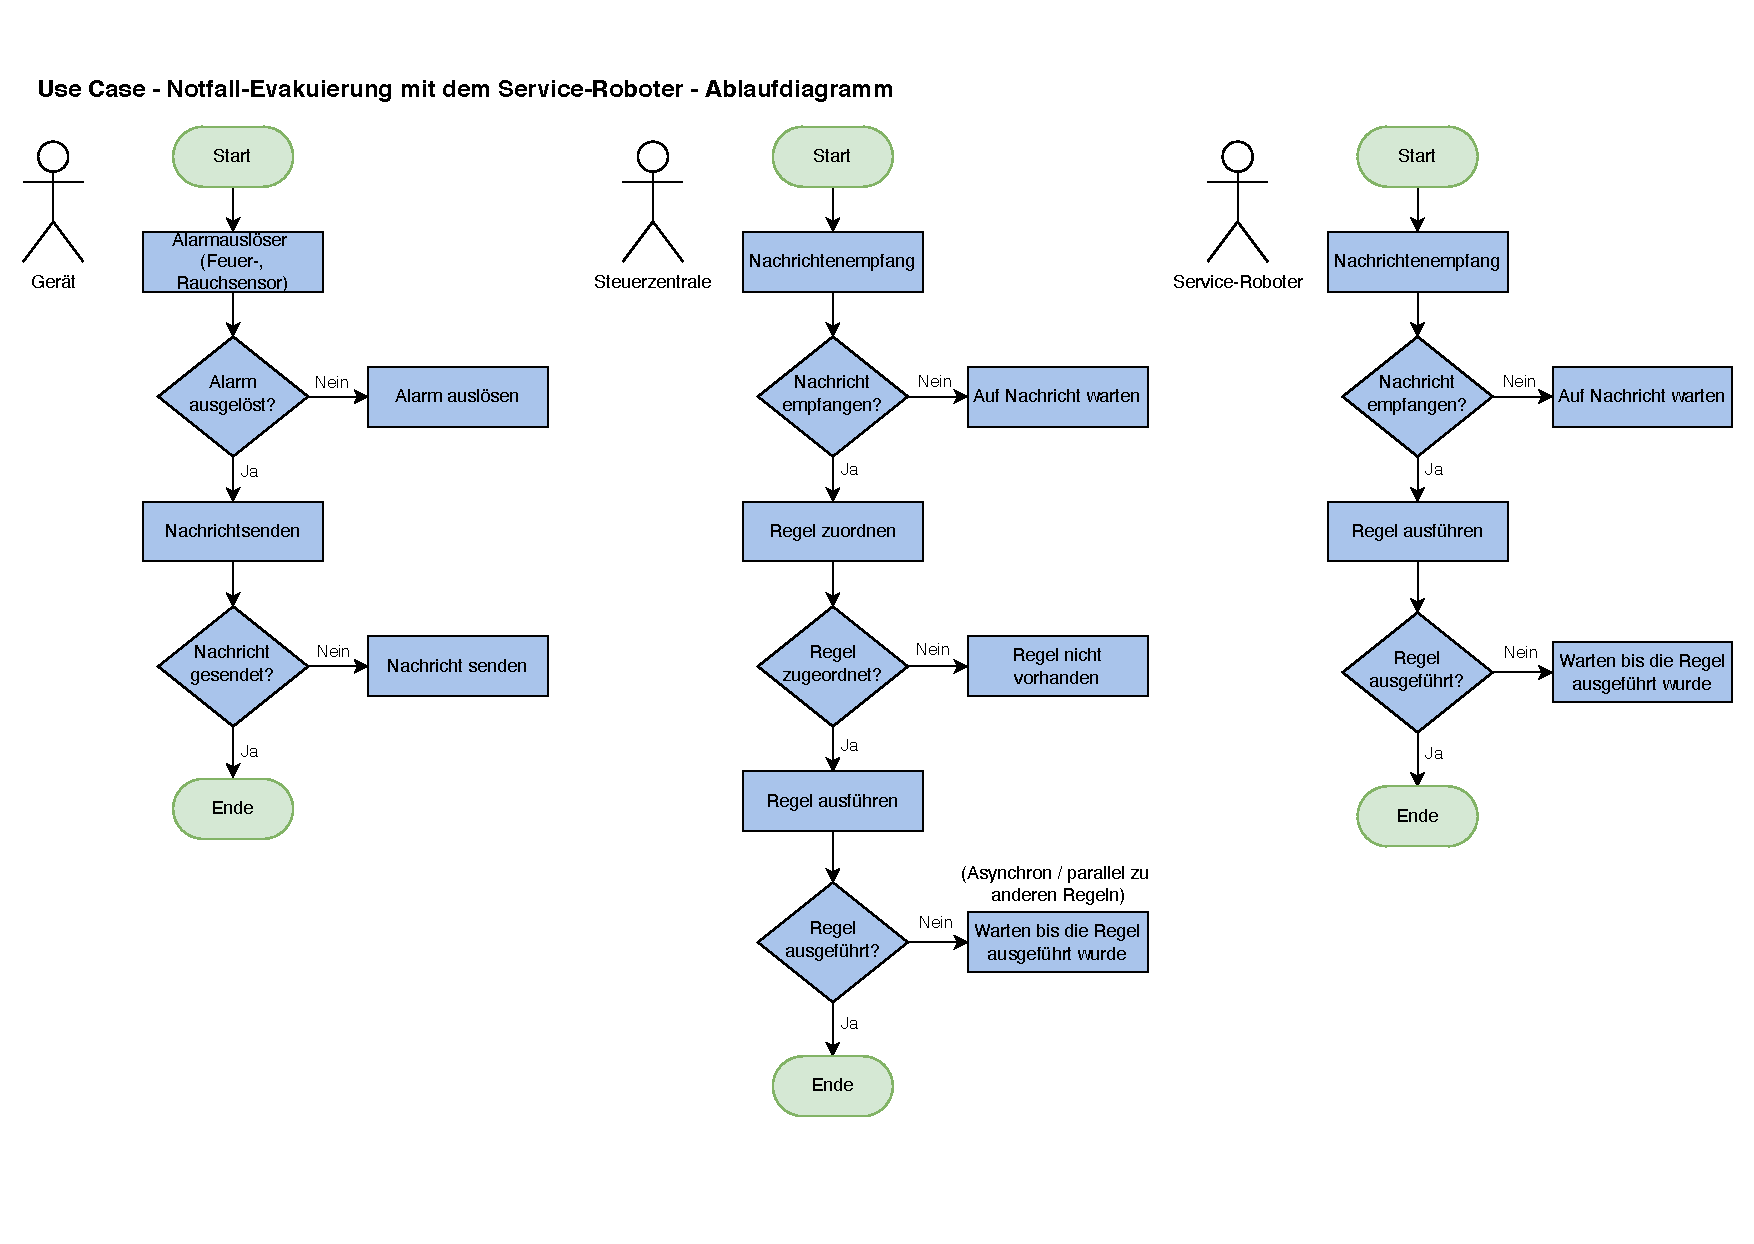
\includepdf[scale=0.75, pages=-, angle=90, fitpaper]{images/UC2_Ablaufdiagramm_Sichtweisen.pdf}
\end{landscape}

\chapter{}
\label{appendix:steuerzentrale}
\begin{lstlisting}[language=Java, frame=lines, xleftmargin=\parindent, style=algoBericht, label={code:switch}, captionpos=b, caption={Regeldefinition der Lichtschaltung}]
@Scope("singleton")
public class RuleLampSwitch extends Rule<InnovationLabKA> {
  ...
  @Override
  @TriggerAnnotation
  public Trigger ruleTrigger(InnovationLabKA state) {
    return Trigger.MQTT;
  }
  
  @Override
  @ConditionAnnotation
  public boolean checkCondition(InnovationLabKA state) {
    return state.isSchalterOn() != state.isLampeOn();
  }
  
  @Override
  @ProcessAnnotation
  public void ruleProcess(InnovationLabKA state) {
    logicHubState.setState((state) -> {
        state.setLampe(state.getSchalter());
    });
  }
  ...
}
\end{lstlisting}
\pagebreak
\label{appendix:hoasAutomation}
\begin{lstlisting}[language=xml, frame=lines, xleftmargin=\parindent, style=algoBericht, label={code:hoasAutomation}, captionpos=b, caption={Regeldefinition der Lichtschaltung über Home Assistant}]
  id: '1632733838684'
  alias: Schalter Kueche Licht An
  description: ''
  trigger:
    - platform: device
      domain: mqtt
      device_id: 7281b0009a1b5a48f077dc0873070ce5
      type: action
      subtype: 'on'
      discovery_id: 0x804b50fffe8f57fc action_on
  condition: []
  action:
    - scene: scene.licht_kuche
  mode: single
\end{lstlisting}

\label{appendix:openhabCode}
\begin{lstlisting}[language=Java, frame=lines, xleftmargin=\parindent, style=algoBericht, label={code:openhabSwitch}, captionpos=b, caption={Regeldefinition der Lichtschaltung via openHAB}]
rule "Ikea_FB_Button" 
when Channel "deconz:switch:XXXXXXXX:XXXXXX:buttonevent"  triggered
         
then
  if (TRADFRIFernbedienungIKEAofSweden_Button.state==5002){
    if (IkeaLight.state==ON) {
      IkeaLight.sendCommand(OFF)
    }
    if (IkeaLight.state==OFF) {
      IkeaLight.sendCommand(ON)
    }
  }
end
\end{lstlisting}

\chapter{}
\label{appendix:usabilitytestpaper}
%\begin{figure}[hbt!]

\includepdf[pages=-, fitpaper]{chapter/9Anhang/Usability-Dokument_MA.pdf}
%  \caption{Dokument zum Usability-Test}
%  \label{appendix:usabilitypaper}
%\end{figure}
%%%%%%%%%%%%%%%%%%%%%%%%%%%%%%%%%%%%%%%%%%%%%%%%%%%%%%%%%%%%%%%%%%%%%%%%%%%%%%%

\newpage
\thispagestyle{empty}
\begin{framed}
\begin{center}
\Large\bfseries Erklärung
\end{center}
\medskip
\noindent
Ich versichere, dass ich diese \Was ~mit dem Thema:
\textit{\enquote{\Titel}}
selbstständig verfasst, keine anderen als die angegebenen Quellen und Hilfsmittel benutzt sowie alle wörtlichen oder sinngemäß übernommenen Stellen in der Arbeit gekennzeichnet habe. 
Die Arbeit wurde noch keiner Kommission zur Prüfung vorgelegt und verletzt in keiner Weise Rechte Dritter.
\vspace{3cm}
\noindent
\underline{\hspace{0cm}}\hfill\underline{\hspace{15cm}}\\
Ort, Datum\hfill Unterschrift\hspace{4cm}
\end{framed}

%%%%%%%%%%%%%%%%%%%%%%%%%%%%%%%%%%%%%%%%%%%%%%%%%%%%%%%%%%%%%%%%%%%%%%%%%%%%%%%
\endinput
%%%%%%%%%%%%%%%%%%%%%%%%%%%%%%%%%%%%%%%%%%%%%%%%%%%%%%%%%%%%%%%%%%%%%%%%%%%%%%%


%%%%%%%%%%%%%%%%%%%%%%%%%%%%%%%%%%%%%%%%%%%%%%%%%%%%%%%%%%%%%%%%%%%%%%%%%%%%%%%

\end{document}
